\documentclass[12pt]{article}
\usepackage[a4paper, margin=25.4mm]{geometry}
\usepackage{graphicx}
\usepackage{float}
\usepackage{tabularx}
\usepackage{array,longtable}
\setlength{\arrayrulewidth}{0.6pt}   % visible table grid; default 0.4pt is too faint
\usepackage{fontspec}
\setmainfont{Times New Roman}
\usepackage{titlesec}
\titleformat{\section}{\centering\fontsize{16}{19}\selectfont\bfseries}{\thesection}{1em}{}
\titleformat{\subsection}{\fontsize{14}{17}\selectfont\bfseries}{\thesubsection}{1em}{}
\usepackage[font=small,labelfont=bf]{caption}
\usepackage{fancyhdr}
\pagestyle{fancy}\fancyhf{}\fancyfoot[R]{\thepage}
\renewcommand{\headrulewidth}{0pt}
\usepackage[hidelinks]{hyperref}
\usepackage{xurl}
\setlength{\emergencystretch}{3em}
\widowpenalty=10000\clubpenalty=10000

% 1.5 Line Spacing Configuration
\usepackage{setspace}
\onehalfspacing
\setlength{\parindent}{0pt}
\setlength{\parskip}{6pt}
\counterwithin{table}{section}
\counterwithin{figure}{section}
\pagenumbering{roman}

\begin{document}
\hypersetup{pageanchor=false}
\begin{titlepage}
	\centering
	% \vspace*{1.5cm}
	\hrulefill\\
	\vspace{0.25cm}
	{\scshape\LARGE Data Science Research Project \par}
	\vspace{0.2cm}
	\hrulefill\\
	\vspace{0.55cm}

	{\normalsize\itshape A final report submitted in partial fulfilment of the requirements for the \par}
	
	\vspace{0.3cm}
	
	{\normalsize\itshape Research Capstone Project \\ \vspace{0.2cm} in \\ \vspace{0.2cm} Master of Data Science\par}
	
	\vspace{0.55cm}
	{\normalsize By \par}
	
	\vspace{0.55cm}
	{\large\itshape Kingsley Ogadinma Onyekwele}
	
	\vspace{4pt}
	{\normalsize SPI240350}
	
	\vspace{0.55cm}
	{\large\itshape Supervisor: Dr Anh Nguyen \par}
    
	\vspace{0.55cm}
	{\normalsize Sydney Polytechnic Institute \\ \vspace{4pt}
	Level 4, 191 Thomas Street, Haymarket, NSW 2000 \\ \vspace{4pt}
	Australia\par}
	\vspace{0.8cm}
	
\includegraphics[width=0.34\linewidth]{misc/spi-logo.png}
	
	\vspace{0.55cm}
	{\normalsize September 2026 \par}

	\vspace{0.35cm}
	{\small\itshape Short-Term Solar PV Forecasting in NSW Using Machine Learning\par}

\end{titlepage}

\hypersetup{pageanchor=true}

\section*{Declaration}
I, \textbf{Kingsley Ogadinma Onyekwele} hereby declare that the work presented in this thesis is the result of my own effort and has not been submitted, either in whole or in part, for any other degree or qualification. Where the work of others has been used, it has been duly acknowledged in the text and listed in the references. This report does not contain material previously published or written by another person, except where due reference is made. Any views expressed are those of the author and do not necessarily reflect those of the Sydney Polytechnic Institute, or any associated organisation.

\begin{flushright}
\vspace{10pt}
Author: Kingsley Ogadinma Onyekwele \\
Signed: \textit{Kingsley Ogadinma Onyekwele} \\
Date: 30 August 2026 \\
\end{flushright}

\clearpage

\begin{center}
\section*{Acknowledgements}
\end{center}

I thank my supervisor, Dr Anh Nguyen, for his guidance throughout this project, from the shaping of the research question through the modelling stages to the preparation of this report. His feedback on scope, on evaluation practice, and on the writing itself shaped the work at every stage, and his insistence on statistical rigour over headline accuracy changed the way the results in this report were established and presented.

I also thank the faculty of the Master of Data Science program at the Sydney Polytechnic Institute for the grounding in machine learning, statistical practice, and research method that this project draws on, and my fellow students in the MDS650 cohort, whose questions during the progression reviews sharpened the research question and kept the project's difficulties in proportion. The progress presentations in particular benefited from colleagues who asked what the results would mean for an operator rather than only for a model.

The solar generation and market data used in this work were obtained from the Australian Energy Market Operator through the NEMOSIS dynamic data compiler, and the meteorological reanalysis from renewables.ninja. I acknowledge both services, and the underlying MERRA-2 project of NASA's Global Modeling and Assimilation Office, for making these datasets openly available. Open data infrastructure of this kind is what allows a reproducible regional benchmark to be assembled, re-executed, and extended by others, and this project depends on it end to end.

Finally, I thank my family for their patience and encouragement across this trimester and throughout the Master of Data Science course.

\clearpage

\section*{Abstract}
This study asks to what extent AEMO five-minute intra-hour features improve short-term solar PV forecast skill over meteorological inputs alone in New South Wales. Five-minute AEMO observations were aggregated into complete hours and aligned with regional hourly MERRA-2 reanalysis. Exact duplicate timestamps were collapsed and conflicting duplicates removed. XGBoost, LSTM, an unpenalised CNN-BiLSTM and a physics-guided CNN-BiLSTM were compared with persistence, rolling climatology and SARIMA at 1, 3, 6 and 24-hour horizons using a chronological 2025 test set. Neural headline forecasts average five seeds.

Without hourly generation history, the two scale-normalised dispersion summaries improve all four learned procedures robustly at every horizon, by 1.26 to 11.46 percent. Once hourly history is controlled, all four procedures gain robustly at one hour, XGBoost and the physics-guided model also gain at three and six hours, and none gains robustly at 24 hours. Robust controlled improvements range from 1.63 to 2.86 percent and require agreement across block intervals, corrected Diebold-Mariano tests and an output-scale sensitivity check.

On combined inputs, LSTM achieves the best one-hour RMSE of 155.25 MW, the physics-guided model leads at three and six hours with 300.28 and 369.17 MW, and the unpenalised CNN-BiLSTM leads at 24 hours with 399.77 MW. A matched comparison attributes a robust 1.18 percent six-hour improvement to the physics-guided loss penalties, but finds no robust penalty effect at the other horizons. The weighted ensemble does not outperform the best neural model.

The evidence supports five-minute variability as a modest short-horizon supplement, not the main source of predictive skill. Conclusions are limited to one held-out year, retrospective weather inputs and utility-scale market-cleared generation.

\clearpage

\newpage

\tableofcontents
\clearpage

\listoffigures

\clearpage

\listoftables

\clearpage
\pagenumbering{arabic}

\section{Introduction}

\subsection{Background and Research Context}

New South Wales (NSW) provides a regional setting for short-term solar photovoltaic (PV) forecasting. Variation in solar output complicates the balance between generation and demand, and forecasts can support scheduling and dispatch by anticipating it \cite{prasad2021prediction}. The target studied here is market-cleared generation: the semi-scheduled solar output AEMO accepts into dispatch after network constraints and price effects, which is not the same as available production. This project examines predictive accuracy; it does not estimate avoided curtailment, balancing costs or financial benefits.

Forecast value depends on lead time and the decision it supports, so the study evaluates one-hour, three-hour, six-hour and day-ahead horizons covering intraday and next-day planning. These are experimental forecasting horizons, not simulations of AEMO scheduling or settlement, and regional MW errors alone cannot establish participant-level costs or savings.

Relevant work includes hierarchical temporal convolutional networks for day-ahead regional forecasting in Western Australia \cite{perera2024dayahead}, transformer models for irradiance and PV power forecasting \cite{schubnel2025solarcross}, \cite{scott2025transformers}, intra-hour solar radiation variability \cite{huang2016intra}, and satellite-based prediction at four Australian locations \cite{prasad2021prediction}. None supplies the matching NSW1 benchmark sought here. NSW exposure to East Coast Low events \cite{bom2022ecl} provides regional context, although this project does not evaluate event-specific errors.

\subsection{Research Problem and Motivation}

The reviewed literature identifies no NSW benchmark combining local meteorological reanalysis with grid data for short-term solar PV generation forecasting. Prior Australian work has forecast at regional or state level from weather data and historical generation, and utility-scale forecasts feed national balancing through AEMO's operational processes, yet the retained review found no study sharing the NSW1 target, source combination and evaluation design. Section 2.1 records that those search notes lack a complete auditable screening ledger, so the gap is bounded by the retained material rather than established against the field. The nearest retained work is Perera et al. \cite{perera2024dayahead}, who forecast distributed rooftop generation in Western Australia, and Prasad and Kay \cite{prasad2021prediction}, who convert satellite-derived irradiance forecasts into power at Queensland and Victorian sites; neither combines NSW1 market-cleared generation with completed-hour AEMO history.

A second constraint is the meteorological source: MERRA-2 is retrospective reanalysis, not an operational forecast \cite{pfenninger2016longterm}. The experiment uses weather information associated with the forecast origin and its history, not archived numerical weather predictions issued in real time, so its value lies in comparing input sets and configurations within a retrospective benchmark. Neither a fixed deployment-error penalty nor unchanged operational model rankings can be inferred.

\subsection{Research Questions and Objectives}

The research question guiding this project is: to what extent do AEMO five-minute intra-hour features improve short-term solar PV forecast skill over meteorological inputs alone in New South Wales?

Three objectives structure the work. The first benchmarks XGBoost, a unidirectional LSTM, an unpenalised CNN-\allowbreak{}BiLSTM and a physics-guided CNN-\allowbreak{}BiLSTM against persistence, rolling climatology and seasonal ARIMA (SARIMA) over 1 h, 3 h, 6 h and 24 h horizons. The second estimates the incremental contribution of two scale-normalised intra-hour variables over meteorological inputs alone, and tests whether it survives once ordinary hourly generation history is present. The third compares the learned procedures and describes whether a validation-weighted ensemble improves their point accuracy. Each uses the same 2025 evaluation year and horizon-specific common forecast windows.

The primary hypothesis is that adding the coefficient of variation and relative five-minute range to a meteorology-only input set reduces RMSE at short horizons. Every learned procedure is fitted on all four feature sets, so the meteorology-only and history-controlled contrasts are estimated across the complete factorial. A gain counts as robust only when the 168-hour moving-block interval excludes zero, Diebold-Mariano tests remain significant after correction under all three dependence bandwidths, and an output-scale-relative sensitivity check agrees in direction. The same factorial estimates the larger contribution of ordinary hourly history.

The architecture comparison includes a matched control: the two CNN-\allowbreak{}BiLSTM procedures share architecture and training, differing only in the two loss penalties. The controlled contrast directly answers whether five-minute summaries add information beyond ordinary hourly history, while the meteorology-only contrast shows their complementary value without that history. The ensemble and regime analyses remain secondary.

The dataset combines hourly renewables.ninja meteorological reanalysis \cite{pfenninger2016longterm}, \cite{renewables2025api} with 5-minute AEMO NEMOSIS dispatch data \cite{aemo2024nemosis} for September 2020 to 2025, engineered into four information sets of up to 16 variables and split chronologically into training (2020 to 2023), validation (2024) and test (2025). After joining, 46,570 complete hourly observations remain, falling to 46,558 once rolling-feature warm-up is removed and before the contiguous-window burn-in described in Section 3.1.

\subsection{Significance and Expected Contribution}

The contribution is ranked. The primary contribution is an attribution of short-horizon forecast skill to AEMO five-minute intra-hour features, measured over meteorological inputs alone and then re-measured once ordinary hourly generation history is present. The supporting contribution is the applied NSW benchmark that makes that attribution possible: a four-set comparison of established architectures on market-cleared NSW1 generation, which the retained literature does not supply. Regime-conditioned errors describe where gains occur but remain exploratory. The novelty claimed is limited to that benchmark and comparison design, not a new forecasting architecture.

For AEMO and practitioners, the benchmark retrospectively compares input choices and established configurations. Its target is market-cleared NSW1 dispatch, excluding most rooftop production; operational application would require archived issue-time weather forecasts, latency checks and a missing-data policy, while extending it to distributed PV would require distributed observations.

The evaluation distinguishes the value of all generation-history predictors from the incremental contribution of their within-hour dispersion.

This distinction matters for both scientific interpretation and system design. If a model improves after all AEMO history is added, the change may simply reflect access to the latest generation level, an unusually strong predictor of near-term output, and not the five-minute sampling frequency. Conversely, a comparison of otherwise identical inputs differing only in intra-hour dispersion can estimate whether variability within the latest completed hour carries information its mean and trailing summaries omit. The two contrasts therefore answer different halves of the research question, and both are reported.

The four forecast horizons represent distinct decisions rather than interchangeable repetitions. One and three hours emphasise near-term cloud and ramp persistence, six hours crosses a substantial part of the daylight cycle, and 24 hours tests day-ahead periodicity.

The study also separates retrospective validity from operational readiness. A chronologically held-out year meaningfully tests temporal generalisation, but reanalysis weather, archived market data and zero assumed delivery delay do not recreate a live forecast service. The report therefore uses terms such as benchmark, association and conditional skill and avoids claiming deployable accuracy, economic savings or causal effects of weather regimes.

\subsection{Thesis Outline}

Chapter 2 synthesises the literature and research gap. Chapter 3 describes the data, models and evaluation design. Chapter 4 presents the results, Chapter 5 interprets them and their limitations, and Chapter 6 states the contribution and future work.

\begin{figure}[!htbp]\centering\small
\begin{tabularx}{\linewidth}{|p{0.24\linewidth}|X|}\hline
1 Introduction & Research question, NSW context, objectives and scope. \\
2 Literature review & Data, algorithms, constraints and evaluation practice. \\
3 Methodology & Controlled features, models, alignment and robust decision rules. \\
4 Results & Baselines, learned models, controlled gains and stability. \\
5 Discussion & Interpretation, relation to literature and limitations. \\
6 Conclusion & Findings, contribution and future validation needs. \\
\hline\end{tabularx}
\caption{Thesis progression from the research question to conclusions.}\label{fig:ch1_1}\end{figure}

\clearpage

\section{Literature Review}
\subsection{Introduction}

This chapter reviews short-term solar photovoltaic generation forecasting with machine learning, focusing on data, model choice and evaluation relevant to New South Wales (NSW). The retained literature did not identify a benchmark matching this project’s NSW1 market-cleared target and combination of reanalysis with completed-hour AEMO generation history.

The review draws on the project's July 2026 search notes. arXiv was queried through 15 Boolean expressions combining terms such as solar PV forecasting, machine learning, irradiance, LSTM, physics-guided and reanalysis. Semantic Scholar was queried through three broader expressions. Coverage ran from 2020 to 2026, with foundational pre-2020 papers retained where they established architectures still in use. Inclusion required machine learning or statistical forecasting of solar irradiance or PV generation with reported quantitative error metrics. Wind-only forecasting, papers without reported metrics, and hardware or policy analysis were excluded. Screening was conducted by a single reviewer, and Appendix C records the flow.

The bibliography holds 37 entries: 30 forecasting studies, six data or service sources and one method reference. Per-record screening decisions were not retained, so the review cannot be reproduced record by record. Its gap statement is therefore bounded by the retained material. Appendix C records the reconciliation.

\subsection{Data Characteristics and Preprocessing}

Two distinctions structure the data literature. Pfenninger and Staffell \cite{pfenninger2016longterm} evaluate hourly PV simulations based on reanalysis and satellite data in Europe. Ramirez Camargo and Schmidt \cite{ramirez2020simulation} compare ERA5-land with MERRA-2-based renewables.ninja output at 57 Chilean plants, finding only modest improvements under their modelling assumptions. These studies motivate historical data use without validating this NSW meteorological aggregation. By contrast, Nielsen et al. \cite{nielsen2021irradiancenet} use satellite sequences for short-term irradiance prediction. The second distinction is temporal: hourly meteorology \cite{renewables2025api} and five-minute AEMO dispatch \cite{aemo2024nemosis} require explicit alignment. AEMO's data model defines the two series as regional aggregated unconstrained intermittent generation forecast and regional aggregated semi-scheduled cleared MW \cite{aemo2026datamodel}. The cleared series is the dispatch outcome, so it sits at or below the unconstrained series, and the gap is a market-clearing effect rather than a weather effect. This project retains completed-hour dispersion summaries alongside hourly history.

Multi-source studies address different information needs. Rabault et al. \cite{rabault2025datafusion} combine reanalysis and satellite products to improve GHI estimates against Norwegian observations; Perera et al. \cite{perera2024dayahead} combine generation and weather across 101 Western Australian PV locations; Prasad and Kay \cite{prasad2021prediction} convert satellite-derived irradiance forecasts into power at Queensland and Victorian sites. Wen et al. \cite{wen2026multisource} combine historical, meteorological and forecast variables with cross-dimensional feature extraction. These complementary inputs do not test the AEMO history contrast used here, and their differing tasks cannot establish one universally sufficient spatial resolution.

\subsection{Algorithms and Modelling Approaches}

The literature spans statistical, boosting, recurrent, transformer and constrained methods, but added complexity must be judged within comparable forecasting tasks.

Architecture rankings depend on the task and comparison. Mukhoty et al. \cite{mukhoty2019seq2seq} report strong LSTM encoder-decoder performance against their forecasting alternatives, while Mollasalehi and Farhadi \cite{mollasalehi2025review} review model prevalence, complexity and execution time rather than establishing a universal accuracy-to-speed winner. Feng et al. \cite{feng2018clustering} report benefits from clustering and model blending, and Perera et al. \cite{perera2022multires} report a 3.81 percent average MASE reduction from forecast combinations against their best individual model. Abdullah and Mohammed \cite{abdullah2026physics} report GHI RMSE of 19.53 W/m2 versus 30.64 W/m2 for attention-based alternatives in Sudan. Their physical guidance includes engineered inputs, so this result does not validate the present non-negativity loss. Hoang \cite{hoang2025efficient} reports transformer R2 of 0.9696, whereas Scott et al. \cite{scott2025transformers} find near-baseline performance with poorer sunny-day results. SolarTformer \cite{basu2026solartransformer} and CT-PatchTST \cite{lu2025ctpatchtst} investigate attention and input relationships, while Sudharshan et al. \cite{sudharshan2026spatiotemporal} combine SARIMA and BiLSTM for seasonal irradiance prediction. The differing targets and protocols prevent a common model ranking.

Australian evidence is narrower. Boland et al. review wind and solar farm output forecasting for the National Electricity Market \cite{boland2022forecasting}, and Farah and Boland forecast individual Australian solar farms at five-minute resolution against clear-sky-index persistence and the model AEMO then used \cite{farah2021time}. Both address farm or portfolio output rather than a regional market-cleared aggregate.

\subsection{System and Architecture Considerations}

Operational constraints receive less attention than accuracy in the reviewed work. Dao et al. \cite{dao2020ensemble} consider ensembles on a Raspberry Pi, while Schubnel et al. \cite{schubnel2025solarcross} use a more demanding multimodal model. Their settings illustrate why deployment cost and available inputs belong alongside accuracy in model selection.

The staged baseline, tree and recurrent comparison tests incremental gains within the project's resources. Transformers are excluded by scope, not evidence of inferiority. The complexity claim in Abdullah and Mohammed \cite{abdullah2026physics} motivates comparison, but one study of engineered physical inputs is not evidence that the present loss penalty causes an improvement.

\subsection{Evaluation Metrics and Experimental Design}

Point-error metrics such as RMSE support model comparison, but do not describe the full distribution of future generation. Voyant et al. \cite{voyant2025nice} motivate evaluating more than one error characteristic. Probabilistic work is already present in the retained literature: SolarCrossFormer \cite{schubnel2025solarcross} produces probabilistic irradiance forecasts. The present study evaluates point forecasts and uncertainty in aggregate performance; its bootstrap intervals are not predictive intervals for individual future hours.

Evaluation choices limit comparisons across studies. Perera et al. \cite{perera2024dayahead} report a statistically significant improvement, so significance testing cannot be presented as absent from the reviewed literature. Pedro and Coimbra \cite{pedro2012assessment} explicitly include persistence and ARIMA, supporting the use of strong target-only baselines here. Scott et al. \cite{scott2025transformers} identify sunny-day degradation, while Prasad and Kay \cite{prasad2021prediction} show that delivery latency affects live forecasts. These findings motivate baseline comparison, paired uncertainty assessment and explicit input timing in the present benchmark. Irradiance and generation also remain distinct targets: Prasad and Kay \cite{prasad2021prediction} model their conversion, whereas this project directly forecasts market-cleared MW. Cross-study errors cannot therefore be treated as comparable effect sizes.

Verification practice is itself codified. Yang et al. set out the requirements for deterministic solar forecast verification \cite{yang2020verification}, and the ROPES guideline makes operational information availability a condition of a credible forecast claim \cite{yang2019guideline}. Scoring against persistence, or its clear-sky-index form, is standard \cite{farah2021time}, and the canonical chain from issue-time numerical weather prediction to PV power across the 1 to 24-hour band is described by Lorenz et al. \cite{lorenz2009irradiance}. Two cautions follow for a reanalysis-based design. Forecast models are often built ex post from observed weather over the target period while practice relies on numerical weather prediction \cite{yang2022historical}, and operational forecasts differ measurably from reanalysis over the same region and metric \cite{huang2018assessing}.

\subsection{Conceptual Framework}

The framework separates three nested information layers from model configuration. Weather and calendar variables form the base; completed-hour history adds the recent level and trajectory; and five-minute dispersion adds variation hidden by the hourly mean. Because history and dispersion describe the same completed hour, dispersion is expected to add more over meteorology alone, less once history is included, and less as the horizon lengthens.

Model family moderates extraction: trees and recurrent networks may use the same signal differently. Physical guidance can enter through engineered variables or the training loss \cite{abdullah2026physics}, but the constrained model changes architecture and loss together, so its ranking cannot isolate either mechanism. The primary estimand is the within-model error change when dispersion is added; architecture and ensemble comparisons are secondary. This follows multi-source practice \cite{perera2024dayahead}, \cite{prasad2021prediction}, \cite{rabault2025datafusion}, \cite{wen2026multisource} without assuming extra physical preprocessing improves accuracy \cite{voyant2025clearsky}.

\subsection{Research Gap and Synthesis}

The reviewed evidence supports testing data integration while treating architecture gains as task-dependent because targets, input availability and protocols prevent a universal ranking \cite{perera2024dayahead}, \cite{scott2025transformers}, \cite{mollasalehi2025review}. The retained studies do not match the present comparison of meteorology-only inputs, hourly generation history and AEMO dispersion features for regional market-cleared solar dispatch in NSW1. Perera et al. \cite{perera2024dayahead} instead forecast distributed rooftop generation in Western Australia. This source-and-target distinction defines an applied contribution, not priority over every use of AEMO data or a new method based on geography alone.

Searches of Crossref, OpenAlex and Semantic Scholar in September 2026 for DISPATCHREGIONSUM, SS\_\allowbreak{}SOLAR\_\allowbreak{}CLEAREDMW, SS\_\allowbreak{}SOLAR\_\allowbreak{}UIGF and semi-scheduled found no peer-reviewed forecast of this regional series. The closest Australian work forecasts individual farms or portfolios \cite{boland2022forecasting}, \cite{farah2021time}. AEMO documents the aggregate's forecasting and dispatch process \cite{aemo2022handbook} but publishes no matching benchmark.

Transfer is limited by different targets and input availability. Much reviewed work predicts irradiance rather than market-cleared MW. Retrospective reanalysis differs from weather forecasts available at operational issue times, so neither a fixed deployment penalty nor unchanged model rankings is established. The present meteorology is not independently validated against local ground-station observations; published validation in other regions \cite{pfenninger2016longterm}, \cite{ramirez2020simulation} motivates the source choice but does not establish local accuracy.

The study joins reanalysis and AEMO data for NSW, compares completed-hour history inputs, and adds paired significance tests. Distributed rooftop forecasting \cite{perera2022multires} remains outside this market-cleared target, which does not cover total NSW solar production.

\clearpage

\section{Research Methodology}

This chapter describes the final, executable forecasting design. Hourly MERRA-2 reanalysis obtained through renewables.ninja \cite{pfenninger2016longterm,renewables2025api} was aligned with five-minute AEMO NSW1 solar cleared generation \cite{aemo2024nemosis}. Four learned procedures, three baselines and a descriptive weighted ensemble were evaluated at 1, 3, 6 and 24-hour horizons. The research-question contrast compares weather\_\allowbreak{}history with combined, testing whether intra-hour variability adds skill after hourly generation history is controlled. The complementary weather versus weather\_\allowbreak{}intra contrast measures its value when ordinary generation history is absent.

\begin{figure}[!htbp]\centering\small
\begin{tabularx}{\linewidth}{|p{0.24\linewidth}|X|}\hline
Acquire and align & Fixed-AEST AEMO clock; complete hourly bins; join regional MERRA-2 at UTC instants. \\
Resolve duplicates & Collapse identical values; drop conflicting timestamp groups and incomplete hours. \\
Engineer predictors & Weather, ordinary hourly history and scale-normalised intra-hour variability. \\
Train and validate & Four learned procedures; three baselines; four direct forecast horizons. \\
Evaluate evidence & Common windows, five neural seeds, paired tests and moving-block intervals. \\
Record execution & Fresh kernel, Apple Silicon MPS, package versions and fixed random seeds. \\
\hline\end{tabularx}
\caption{Research workflow implemented by the notebook.}\label{fig:ch3_1}\end{figure}

\subsection{Data Sources and Target}

The target is SS\_\allowbreak{}SOLAR\_\allowbreak{}CLEAREDMW from AEMO's DISPATCHREGIONSUM archive, filtered to NSW1. It is market-cleared utility-scale solar generation, not total NSW production: most rooftop PV is absent, while curtailment and other dispatch effects remain. Intervention labels were unavailable in the legacy export. Hourly meteorology comprises regional means over eight NSW locations. The renewables.ninja simulated electricity series, AEMO UIGF, semi-scheduled aggregates and all target-time generation fields are excluded.

The AEMO market clock is fixed AEST (UTC+10), including legacy records labelled UTC. Five-minute interval-ending observations are assigned to right-closed hourly bins labelled by their left edge, and an hour is retained only when the target column has twelve observations. Night-time zeros are valid; incomplete hours are not. The hour-of-day and day-of-year encodings and the rolling climatology hour key are taken from the index after conversion to Australia/Sydney. These features follow the civil calendar, which is one hour ahead of the market clock during daylight saving, rather than the market clock itself.

Duplicate handling is deliberately conservative. Of 3,532 duplicated timestamp groups, 2,619 hold identical target values and collapse to one observation; the 913 with conflicting values are dropped rather than averaged, as the archive does not identify the normal-dispatch row. The window holds 46,752 hours, of which 46,570 are retained and 182 are lost. Sixty of those are lost at the front: 731 five-minute rows in the first 61 hours carry no market-cleared value, and the resampling grid begins at the first non-null timestamp, so those hours never enter the record. The remaining 122 are incomplete bins: 120 affected by the conflicting duplicates and two others, being the trailing hour of the null run (two of twelve intervals present) and the final hour of the window (eleven of twelve). Reporting the two mechanisms separately avoids attributing the whole loss to duplicate handling.

After cleaning and joining, 46,570 complete hourly observations remain. The chronological split uses Sydney calendar years: September 2020-2023 for training, 2024 for validation and 2025 for testing. Removing rolling-feature warm-up rows leaves 29,016, 8,782 and 8,760 rows in the three splits, within which 118 hours are excluded inside training, two inside validation and none inside test, as the excluded hours fall in the earlier years.

A contiguous 24-hour input window ending h hours before its target removes the first 23 + h rows of a split, so burn-in varies by horizon: 24, 26, 29 and 47 rows at 1, 3, 6 and 24 hours. The "common window" language in Chapter 4 therefore means common across models within a horizon, not identical across horizons.

\begingroup\setlength{\tabcolsep}{3.5pt}\renewcommand{\arraystretch}{1.1}
\newcolumntype{L}[1]{>{\raggedright\arraybackslash}p{#1\linewidth}}
\begin{longtable}{|L{0.30000}|L{0.30000}|L{0.30000}|}
\caption{Test-sample accounting by forecast horizon. Burn-in rows are removed from the front of the 8,760-row test split before any model is scored.}\label{tab:ch3_1}\\
\hline
\textbf{Horizon (h)} & \textbf{Window burn-in rows (23 + h)} & \textbf{Scored test observations} \\ \hline
\endfirsthead
\multicolumn{3}{|l|}{\small Table 3.1 continued}\\ \hline
\textbf{Horizon (h)} & \textbf{Window burn-in rows (23 + h)} & \textbf{Scored test observations} \\ \hline
\endhead
\hline\endfoot
1 & 24 & 8,736 \\ \hline
3 & 26 & 8,734 \\ \hline
6 & 29 & 8,731 \\ \hline
24 & 47 & 8,713 \\ \hline
\end{longtable}\endgroup

The validation year serves model selection and early stopping; the test year is reserved for final comparison. The split also reflects changing utility-scale capacity: a random partition would mix later high-output observations into training and understate the challenge of a growing fleet.

\subsection{Feature Engineering and Forecast Alignment}

Four feature sets isolate different information sources. weather contains 11 predictors: six meteorological variables, a clearness index and sine/cosine encodings of hour and day of year. weather\_\allowbreak{}history adds the latest completed hourly value plus 24-observation trailing mean and standard deviation, giving 14 predictors. weather\_\allowbreak{}intra adds two scale-normalised five-minute summaries, the coefficient of variation and relative range, giving 13 predictors. combined contains all 16.

The intra-hour measures come from the twelve five-minute observations in the latest completed hour. Scaling both summaries by the corresponding hourly level reduces their dependence on the expanding NSW solar fleet, and denominators are protected near zero. They remain retrospective: no observation from the forecast target hour is used.

The clearness index divides GHI by an extraterrestrial horizontal irradiance approximation at a representative NSW coordinate, clipped to [0, 1.5] and zeroed when the denominator is at most 20 W/m2. It is a regional proxy, not a physical ceiling on output.

Each model receives a contiguous 24-hour input window and predicts one scalar target at one horizon, matched by elapsed timestamps rather than row position. Windows crossing a missing hour or a split boundary are rejected, so no nominal 24-row sequence spans more than 24 elapsed hours. Contiguity is enforced on elapsed time, not on local clock time, so a window may span a daylight-saving transition where no hour is missing.

Feature construction follows forecast-time availability. Weather and calendar fields describe the issue-time sequence; generation features end at the latest completed AEMO hour, and trailing statistics are shifted before joining to future targets. Split-specific windowing stops a recurrent context importing observations across a split boundary, and assertions check monotonic unique timestamps, horizon displacement, feature counts and identical targets across feature sets. At the 24-hour horizon, 28,490 training windows remain.

\subsection{Models and Baselines}

XGBoost hyperparameters are selected with 30 Optuna trials per horizon. Each trial fits the same proposed settings on all four feature sets and minimises their mean validation RMSE, including the number of trees as a tuned parameter. The selected settings are then held fixed across all four arms. This feature-set-neutral objective prevents either side of an ablation from receiving its own tuning advantage, while keeping the comparison conditional on one shared configuration.

Direct horizon-specific fitting avoids requiring one model to compromise among targets with different dynamics, at the cost of a larger training matrix and no information sharing among horizons. XGBoost sequences are flattened so lag position remains explicit to the tree learner; for recurrent models, that information stays ordered as time steps.

The LSTM has one recurrent layer with 64 hidden units. The CNN-\allowbreak{}BiLSTM applies a 32-filter one-dimensional convolution with kernel size three, ReLU activation and max pooling, then a one-layer bidirectional LSTM with 64 hidden units and a 128-unit prediction head. Its matched physics-guided version has the same architecture, inputs, optimiser, seeds and early-stopping rule, but adds weight 0.1 on penalties for negative output and departure from zero in known night-time target periods. Their comparison therefore isolates the predictive effect of the tested loss penalties. Comparisons with the LSTM still change several architectural components together.

Neural predictors and targets are standardised using training-window statistics only. Training uses batch size 512, learning rate 0.001, 100 epochs maximum and patience 20, restoring the best validation checkpoint. Each block is trained at seeds 42, 123, 456, 789 and 1024; headline predictions average the five seed forecasts, and individual-seed RMSE mean and standard deviation are reported separately. All three neural procedures use all four feature sets, so both intra-hour contrasts cover every learned procedure.

Persistence repeats the latest completed-hour generation value. Rolling climatology uses only previously available observations for the same target local hour, with a 365-observation trailing window and an availability check. SARIMA(1,1,1)(1,0,0,24) is fitted on the training series, extended through validation, and updated with observations available at each test issue time before forecasting.

The descriptive ensemble combines XGBoost, LSTM, CNN-\allowbreak{}BiLSTM and physics-guided forecasts using inverse-validation-RMSE weights normalised to one, ranging from 0.22 to 0.26. It is excluded from confirmatory significance families because it derives from those components.

\subsection{Evaluation and Statistical Decision Rules}

RMSE in MW is the primary accuracy measure, alongside MAE, bias, R2, daylight RMSE, persistence skill, relative RMSE (dividing by a past-only output scale available at issue time) and peak-normalised RMSE (dividing by an observed peak reference). The share of predictions clipped at zero is reported because non-negativity post-processing can hide negative forecasts.

Meteorology-only gain is 100 x (RMSE\_\allowbreak{}weather - RMSE\_\allowbreak{}weather\_\allowbreak{}intra) / RMSE\_\allowbreak{}weather and controlled feature gain is 100 x (RMSE\_\allowbreak{}weather\_\allowbreak{}history - RMSE\_\allowbreak{}combined) / RMSE\_\allowbreak{}weather\_\allowbreak{}history; a positive value favours intra-hour predictors. Moving-block bootstrap intervals use 2,000 resamples and block lengths of 24, 48 and 168 hours, the last the conservative headline because it preserves a full week of serial structure.

Paired Diebold-Mariano tests \cite{diebold1995comparing} use squared-error differences and Newey-West estimates at bandwidths h-1, 24 and 168 hours. Bonferroni correction is applied separately within each comparison and bandwidth: 16 meteorology-only feature, 16 controlled feature, 48 baseline and 24 pairwise learned-procedure tests. A feature finding is robust only when the 168-hour interval excludes zero, all three corrected tests agree, and the output-scale calculation gives the same direction.

The four inferential families answer different questions. Two evaluate the added intra-hour variables without and with hourly history; the baseline family asks whether each learned procedure improves on persistence, rolling climatology and SARIMA; and the pairwise family compares procedures on combined inputs. Keeping them separate controls multiplicity without placing the descriptive ensemble or regime plots inside a confirmatory family.

The matched CNN-\allowbreak{}BiLSTM pair is the only architecture-level comparison. The other pairwise results concern complete forecasting procedures because model form, training dynamics or seed treatment differ together. Moving-block and Diebold-Mariano calculations treat each saved forecast series as fixed, so their uncertainty covers time dependence within 2025 rather than variation across training seeds.

\subsection{Reproducibility and Ethics}

The final notebook ran from a fresh kernel with code-cell execution counts 1-30 and no recorded errors or standard-error output, from 01:47:44 to 02:38:01 UTC on 14 September 2026 on Apple Silicon (arm64) under PyTorch MPS. The saved environment was conda spunky, Python 3.12.12, PyTorch 2.5.1, XGBoost 3.0.1, pandas 2.3.3 and NumPy 2.1.3. The run records 480 XGBoost tuning fits and 240 neural fits.

The project uses observational agency data without human subjects or personal identifiers. Reproducibility is computational rather than exact across hardware: floating-point order, accelerator kernels and package versions produce small differences. Data-source acknowledgement does not establish redistribution rights \cite{pfenninger2016longterm}, \cite{renewables2025api}, \cite{aemo2024nemosis}.

\clearpage

\section{Analysis, Experiments and Results}

All results come from the clean Apple Silicon execution of Section 3.5, using the common 2025 test window throughout. Neural headline metrics score the average of five seed forecasts; individual-seed dispersion is reported separately.

\subsection{Data Characteristics}

The cleaned series contains 46,570 complete hours. Generation is zero-inflated, strongly diurnal and seasonally structured. Capacity growth and market constraints make the target non-stationary, so these plots describe market-cleared generation rather than a fixed physical production distribution.

\begin{figure}[!htbp]\centering
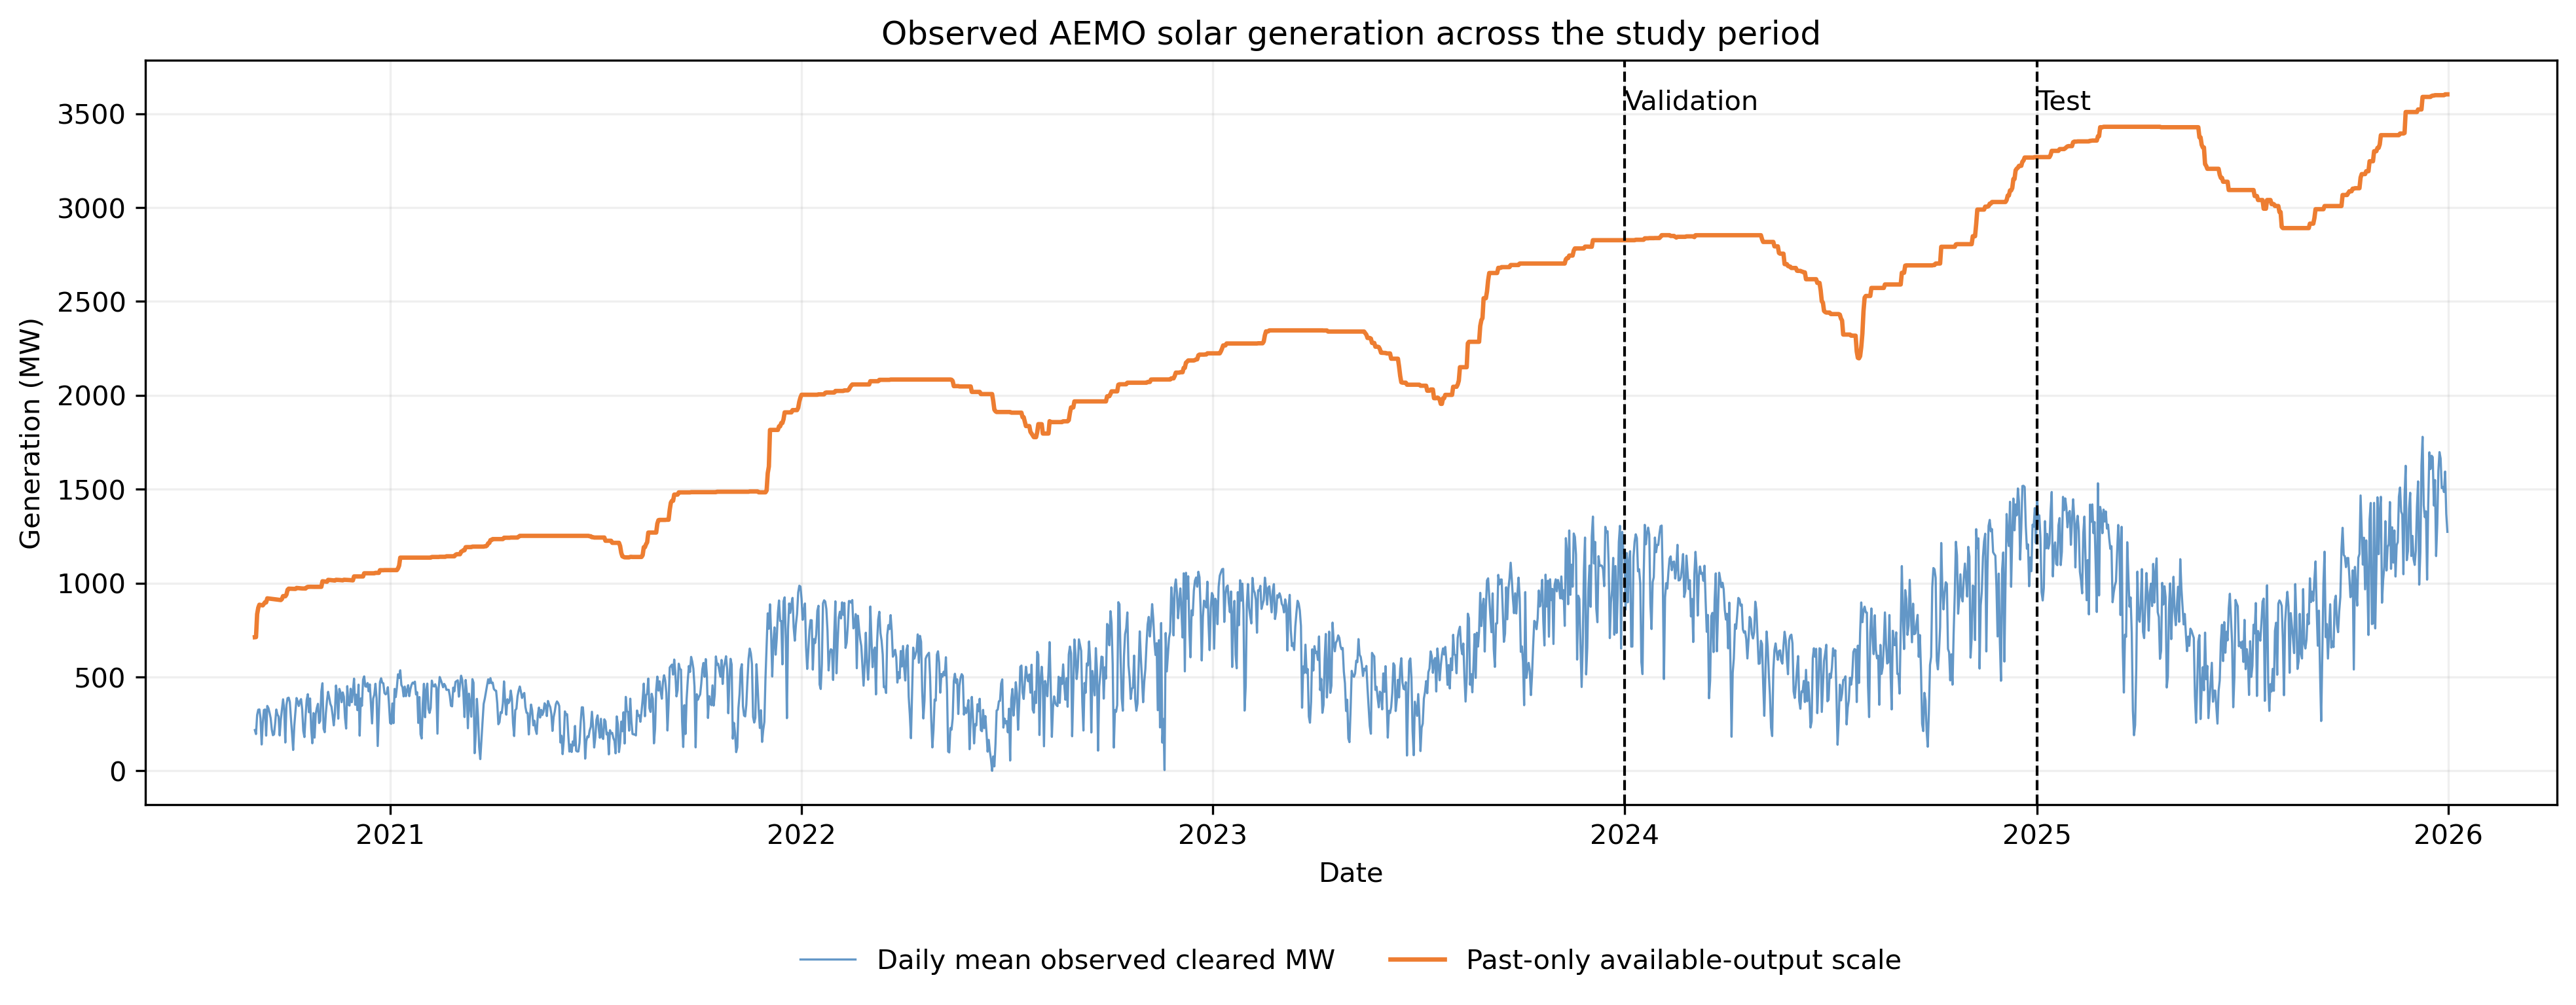
\includegraphics[width=\linewidth,height=0.46\textheight,keepaspectratio]{figures/eda/actual_generation_timeline.png}
\caption[Hourly NSW1 solar generation across the observation period.]{Hourly NSW1 market-cleared solar generation across the observation period.}\label{fig:ch4_1}\end{figure}

\begin{figure}[!htbp]\centering
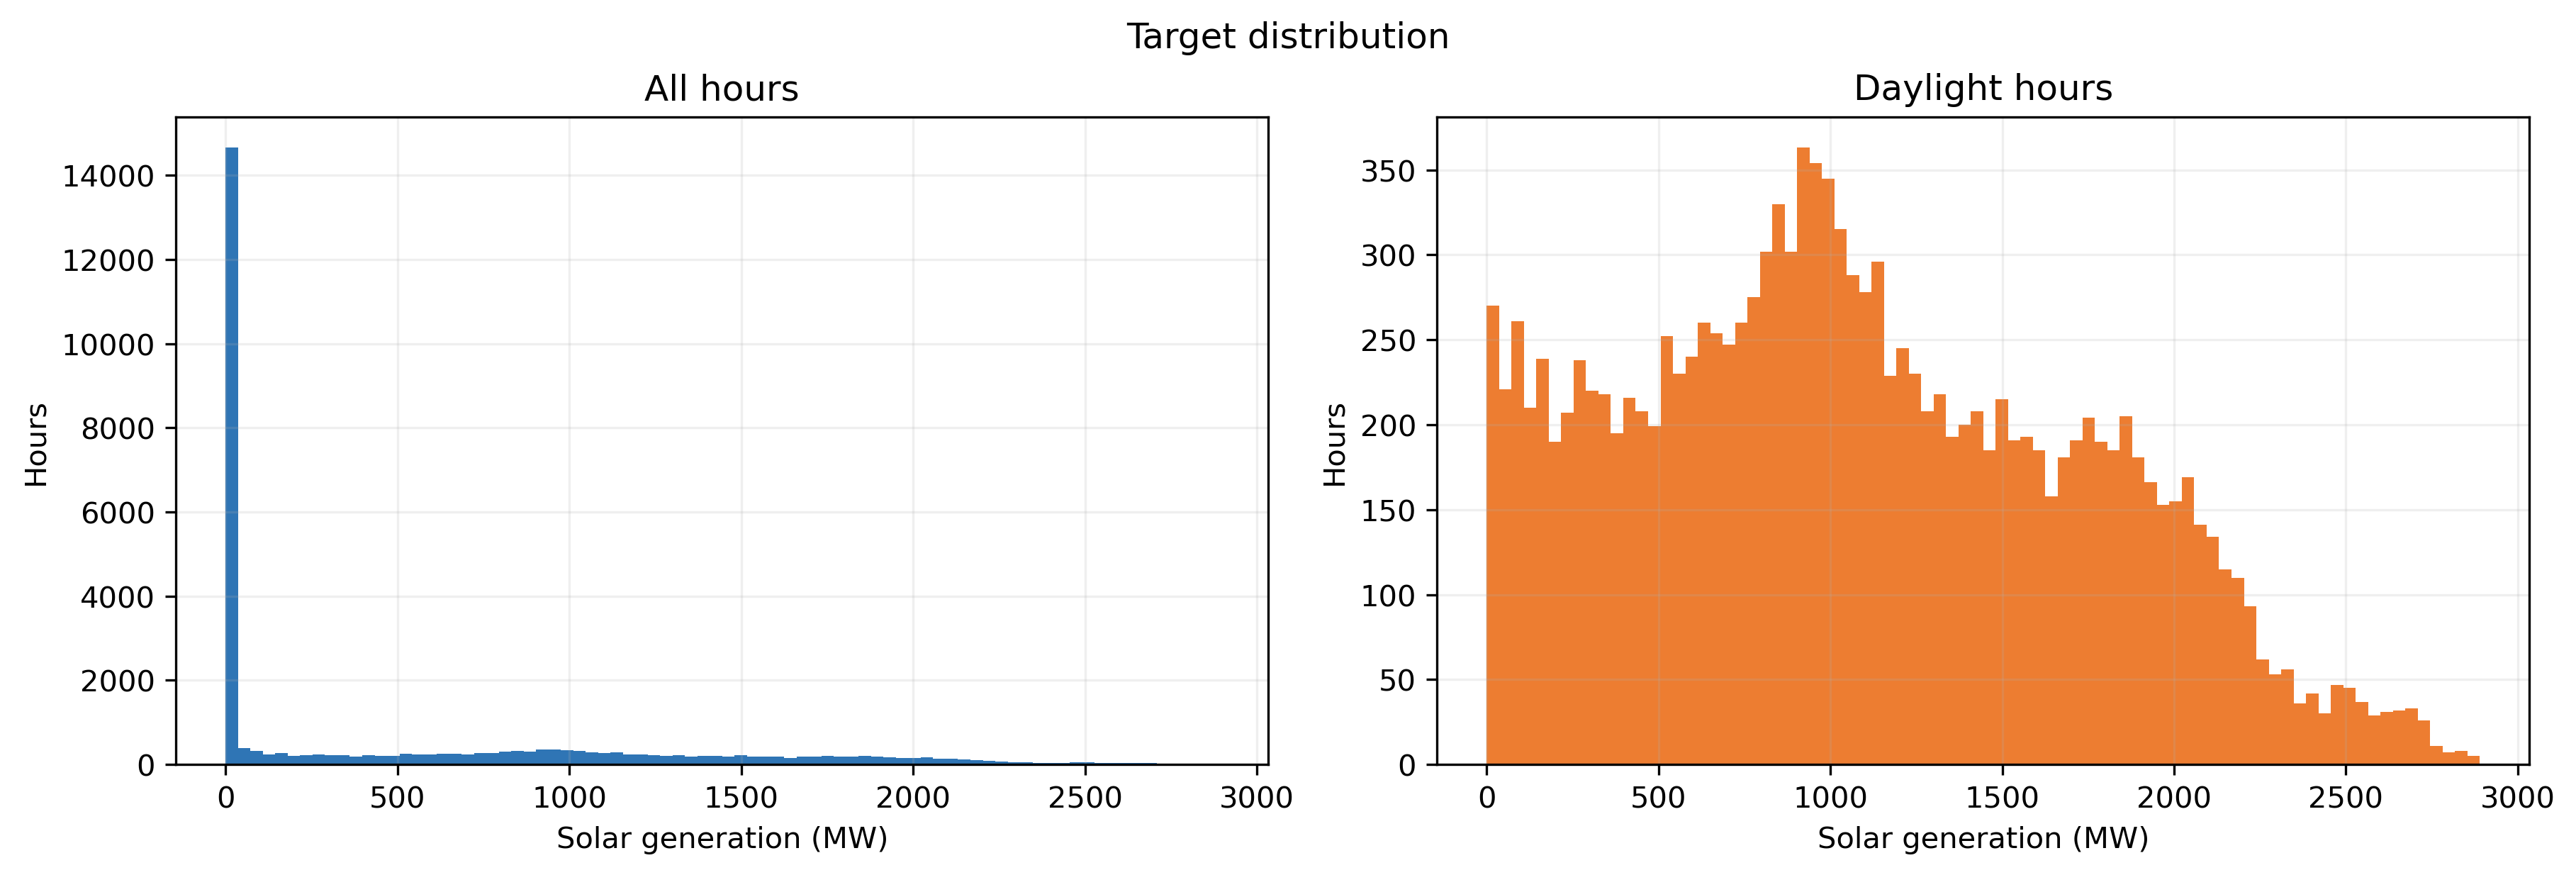
\includegraphics[width=\linewidth,height=0.46\textheight,keepaspectratio]{figures/eda/target_distribution.png}
\caption[Distribution of hourly NSW1 solar generation.]{Distribution of hourly NSW1 market-cleared solar generation, including valid zero output.}\label{fig:ch4_2}\end{figure}

Mean output follows the solar day, while seasonal profile width and level vary across the year. The split diagnostic shows 2025 is not exchangeable with earlier years, supporting chronological rather than random evaluation.

\begin{figure}[!htbp]\centering
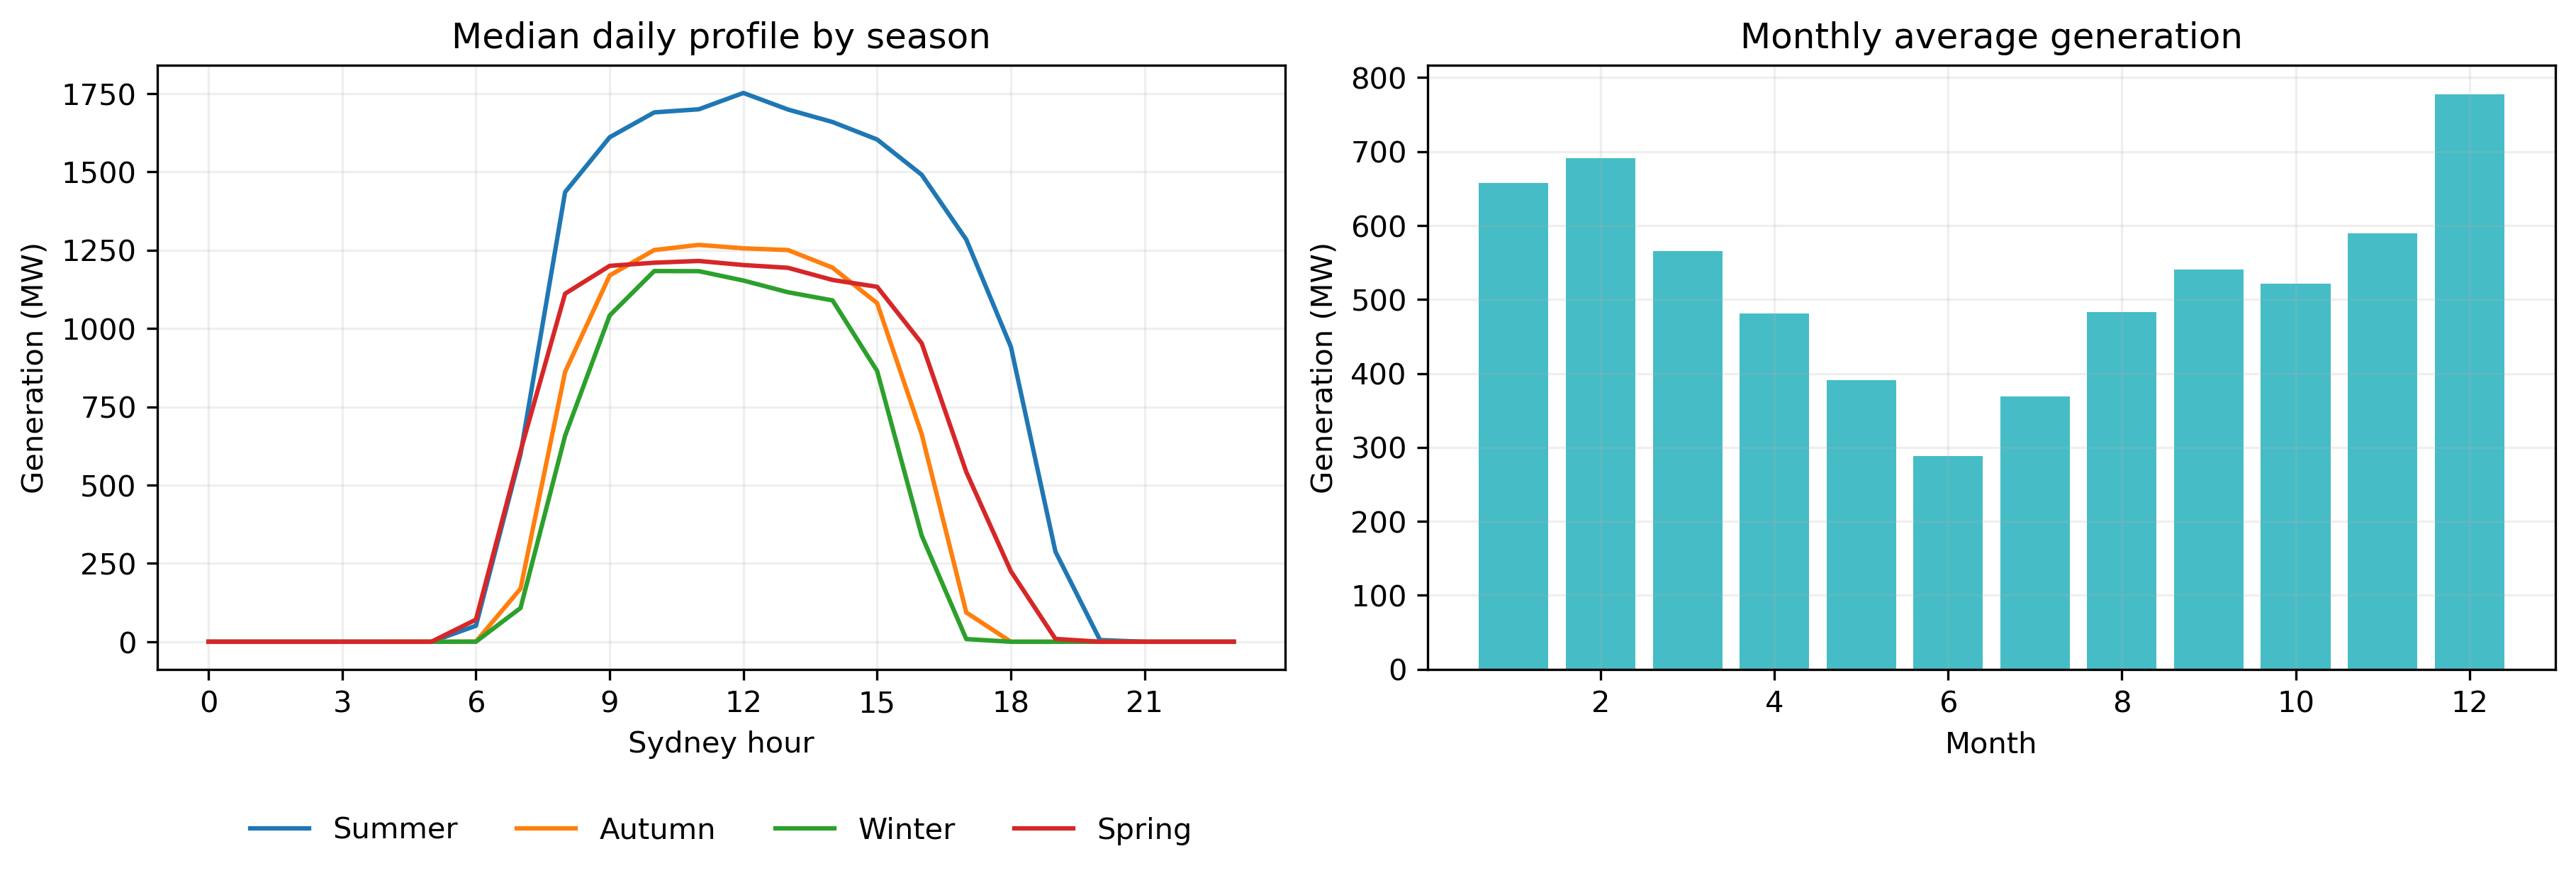
\includegraphics[width=\linewidth,height=0.46\textheight,keepaspectratio]{figures/eda/hourly_seasonal_patterns.png}
\caption[Hourly and seasonal patterns in NSW1 solar generation.]{Hourly and seasonal structure in NSW1 market-cleared solar generation.}\label{fig:ch4_3}\end{figure}

\begin{figure}[!htbp]\centering
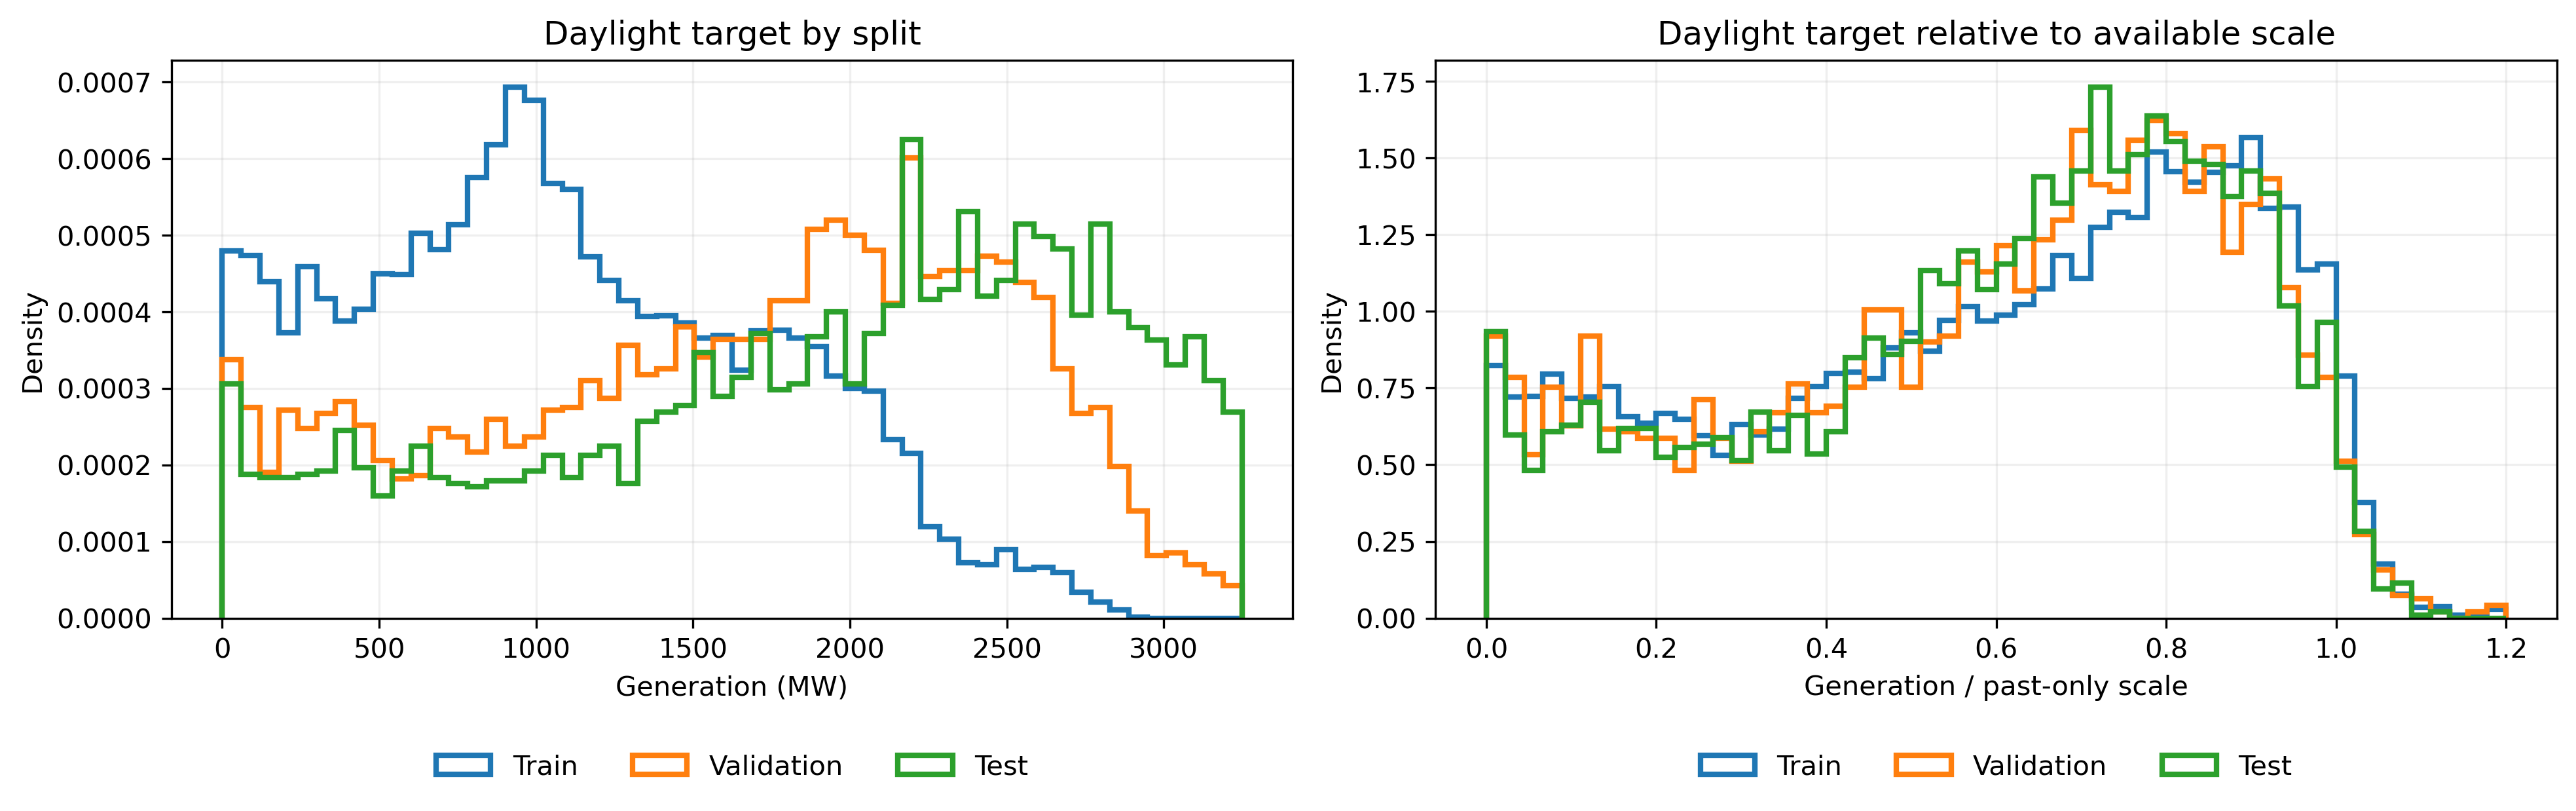
\includegraphics[width=\linewidth,height=0.46\textheight,keepaspectratio]{figures/eda/target_split_drift.png}
\caption[Target distribution across chronological data splits.]{Target distribution across chronological training, validation and test splits.}\label{fig:ch4_4}\end{figure}

Measured output also trends upward, which matters for comparability between splits.

\begin{figure}[!htbp]\centering
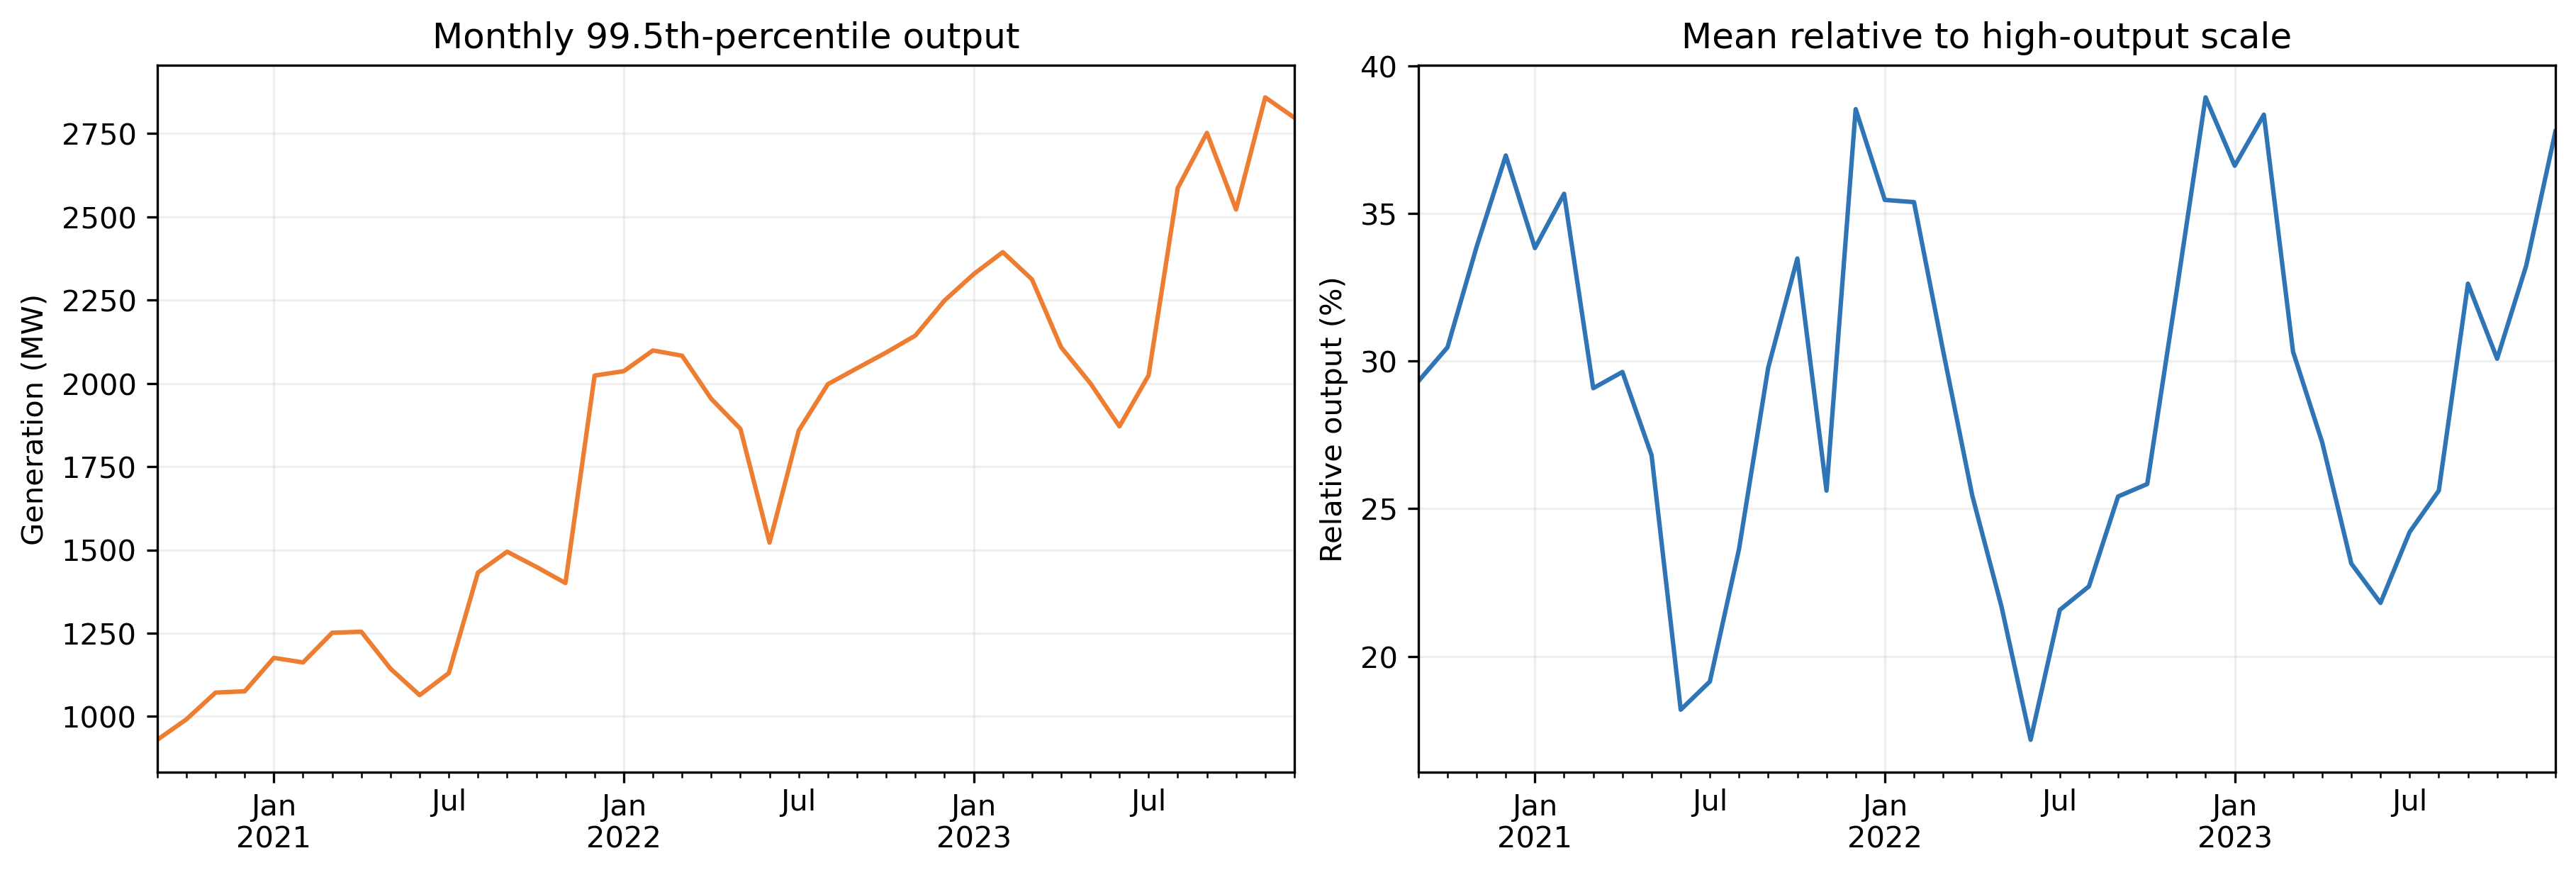
\includegraphics[width=\linewidth,height=0.46\textheight,keepaspectratio]{figures/observed_output_scale.png}
\caption[Monthly observed output scale and mean generation.]{Monthly 99.5th-percentile observed output and mean generation relative to that scale. The level trend documents fleet growth that the past-only output scale is designed to absorb.}\label{fig:ch4_5}\end{figure}

The five-minute source retains fluctuations hidden by hourly averaging. Its scale-normalised coefficient of variation and relative range are the candidate incremental predictors; their relationship with the next-hour ramp motivates the experiment but is not causal evidence.

\begin{figure}[!htbp]\centering
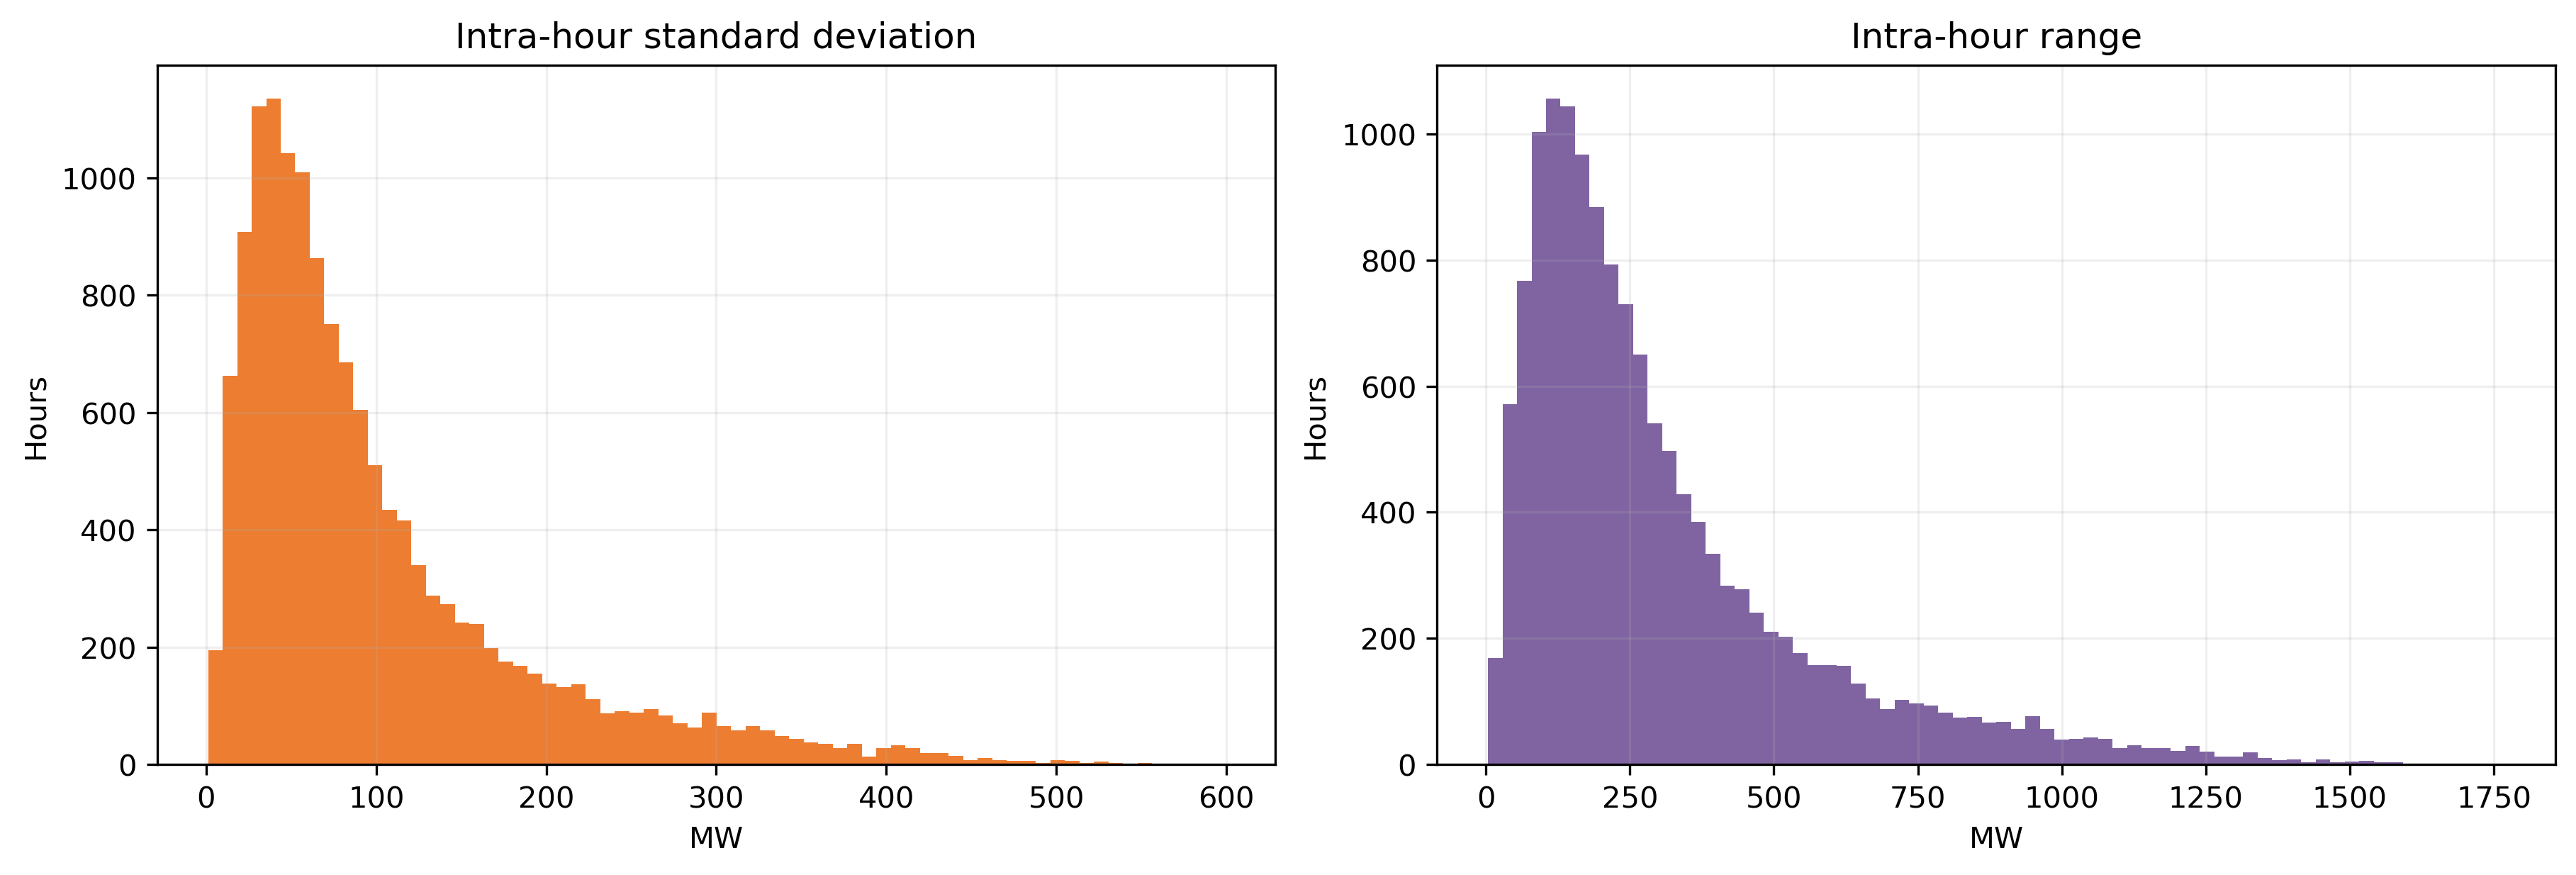
\includegraphics[width=\linewidth,height=0.46\textheight,keepaspectratio]{figures/eda/intra_hour_variability.png}
\caption[Within-hour variability in five-minute AEMO observations.]{Within-hour variability retained from five-minute AEMO observations.}\label{fig:ch4_6}\end{figure}

\begin{figure}[!htbp]\centering
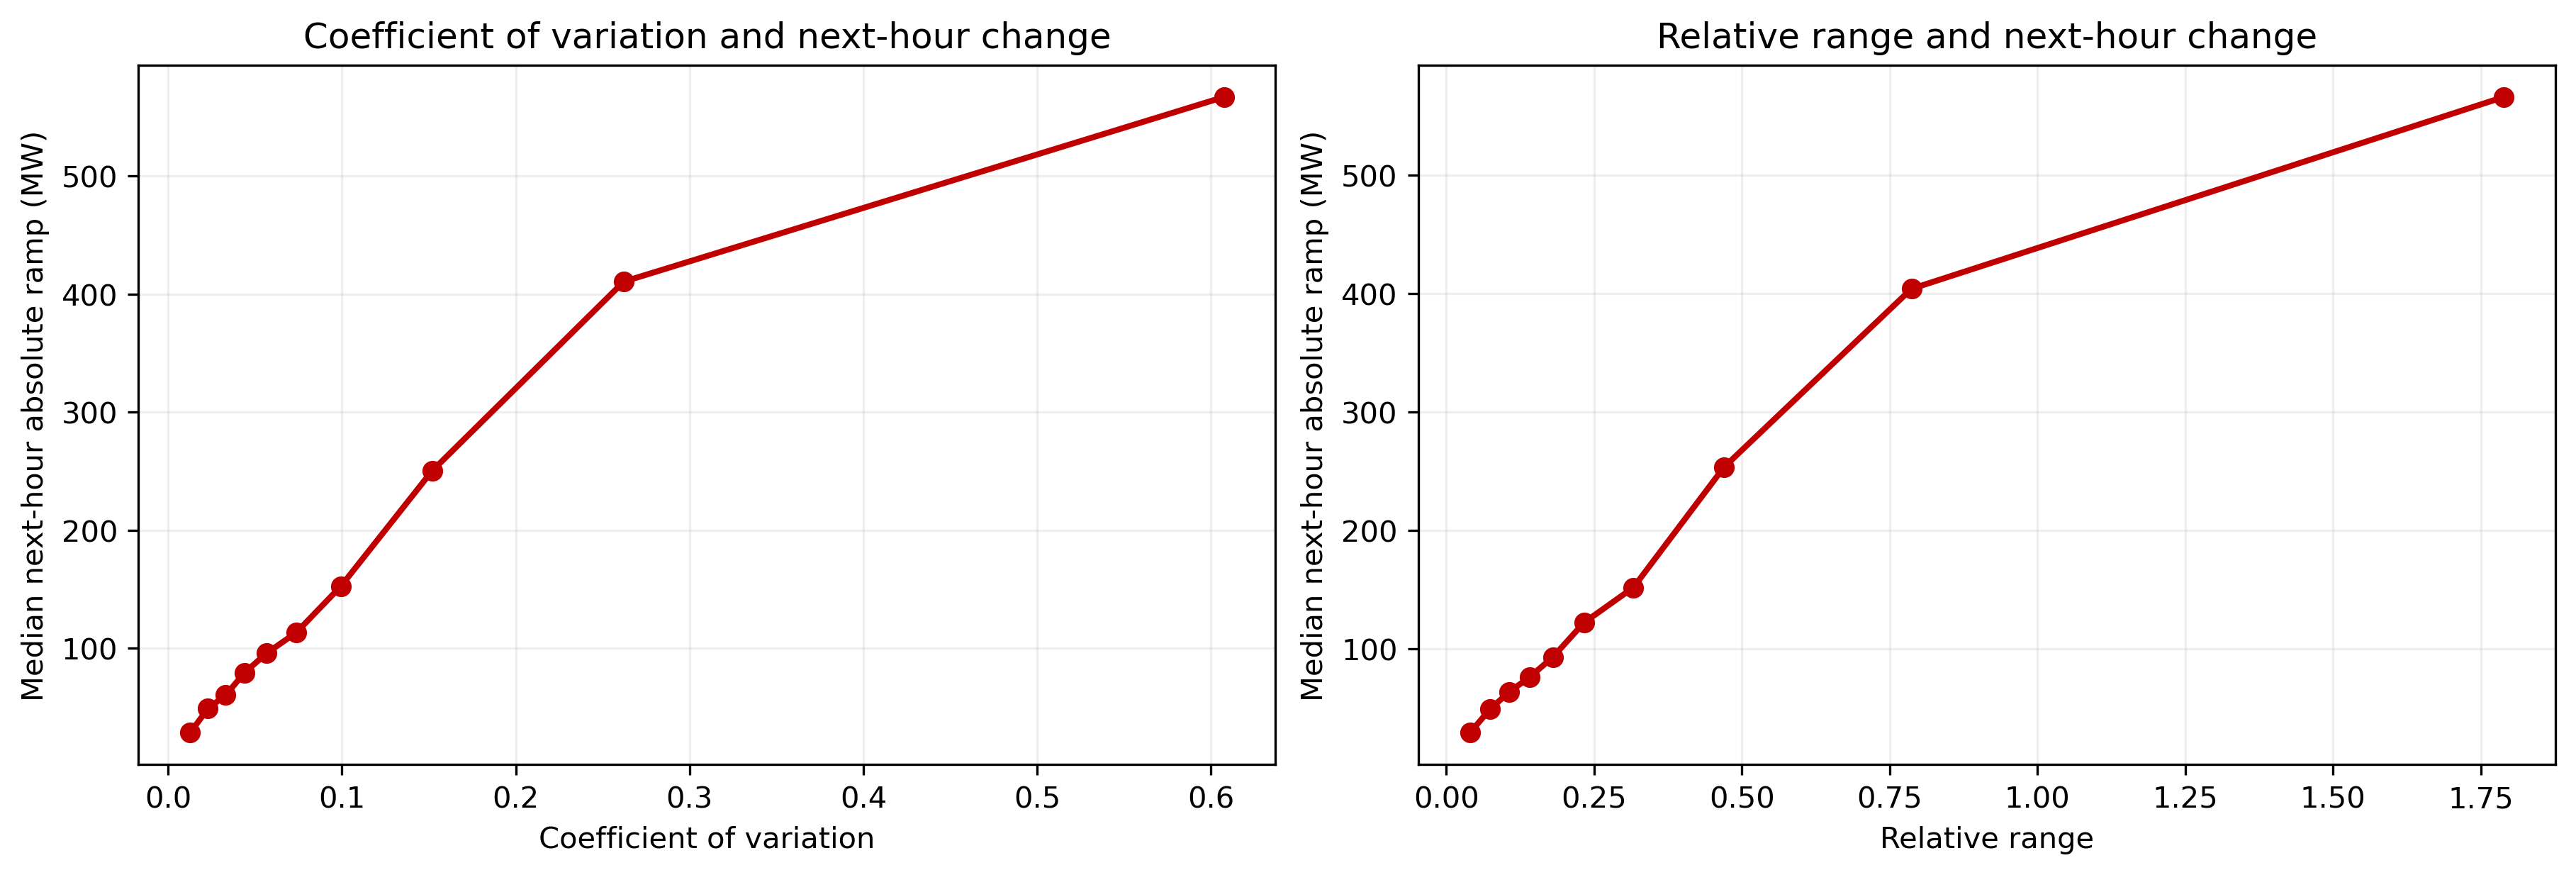
\includegraphics[width=\linewidth,height=0.46\textheight,keepaspectratio]{figures/eda/intra_hour_signal_next_ramp.png}
\caption[Intra-hour variability and the next-hour ramp.]{Association between scale-normalised intra-hour variability and the next-hour ramp.}\label{fig:ch4_7}\end{figure}

The exploratory sequence supports three decisions. Zero output is retained because night-time behaviour belongs to the forecasting problem and the physics-guided loss. Visible split drift justifies past-only scaling instead of a full-sample maximum, and the monotone rise in next-hour change across variability bins makes an incremental short-horizon signal plausible. None of this selects a winning model; that rests on the held-out paired comparisons.

\subsection{Baseline Performance}

Persistence is competitive at 24 hours through daily periodicity but weak at 3 and 6 hours across the daytime rise and fall. SARIMA is the strongest baseline at 1-6 hours; rolling climatology is stable across horizons.

The magnitude of the contrast is substantial. Persistence RMSE rises from 469.06 MW at one hour to 1,631.92 MW at six hours, then falls to 423.60 MW at 24 hours. This U-shape reflects the difference between copying the latest output across the intraday solar cycle and copying it to the same time the next day. Rolling climatology stays close to 571 MW because its same-hour average does not change its information with horizon. SARIMA reaches 221.69 MW at one hour and 433.32 MW at three hours, making a target-only time-series model a demanding comparator without weather fields.

\begingroup\setlength{\tabcolsep}{3.5pt}\renewcommand{\arraystretch}{1.1}
\newcolumntype{L}[1]{>{\raggedright\arraybackslash}p{#1\linewidth}}
\begin{longtable}{|L{0.22500}|L{0.16200}|L{0.11700}|L{0.13500}|L{0.12600}|L{0.13500}|}
\caption{Baseline performance on the common 2025 test window. RMSE and MAE are MW.}\label{tab:ch4_1}\\
\hline
\textbf{Model} & \textbf{h} & \textbf{RMSE} & \textbf{MAE} & \textbf{R2} & \textbf{Persistence skill (\%)} \\ \hline
\endfirsthead
\multicolumn{6}{|l|}{\small Table 4.1 continued}\\ \hline
\textbf{Model} & \textbf{h} & \textbf{RMSE} & \textbf{MAE} & \textbf{R2} & \textbf{Persistence skill (\%)} \\ \hline
\endhead
\hline\endfoot
Persistence & 1 & 469.06 & 242.10 & 0.84 & 0.00 \\ \hline
Persistence & 3 & 1092.77 & 658.82 & 0.13 & 0.00 \\ \hline
Persistence & 6 & 1631.92 & 1210.27 & -0.94 & 0.00 \\ \hline
Persistence & 24 & 423.60 & 219.52 & 0.87 & 0.00 \\ \hline
Rolling climatology & 1 & 570.93 & 348.28 & 0.76 & -21.72 \\ \hline
Rolling climatology & 3 & 570.99 & 348.36 & 0.76 & 47.75 \\ \hline
Rolling climatology & 6 & 571.09 & 348.47 & 0.76 & 65.01 \\ \hline
Rolling climatology & 24 & 570.37 & 347.76 & 0.76 & -34.65 \\ \hline
SARIMA & 1 & 221.69 & 118.13 & 0.96 & 52.74 \\ \hline
SARIMA & 3 & 433.32 & 245.14 & 0.86 & 60.35 \\ \hline
SARIMA & 6 & 542.53 & 343.98 & 0.79 & 66.76 \\ \hline
SARIMA & 24 & 634.49 & 330.15 & 0.71 & -49.78 \\ \hline
\end{longtable}\endgroup

Baseline skill relative to persistence must therefore be read with the horizon. Rolling climatology is 21.72 percent worse at one hour but 65.01 percent better at six hours. SARIMA improves by 52.74-66.76 percent at one to six hours yet is 49.78 percent worse at 24 hours. A single baseline or horizon average would conceal these reversals.

\begin{figure}[!htbp]\centering
\vspace{12pt}
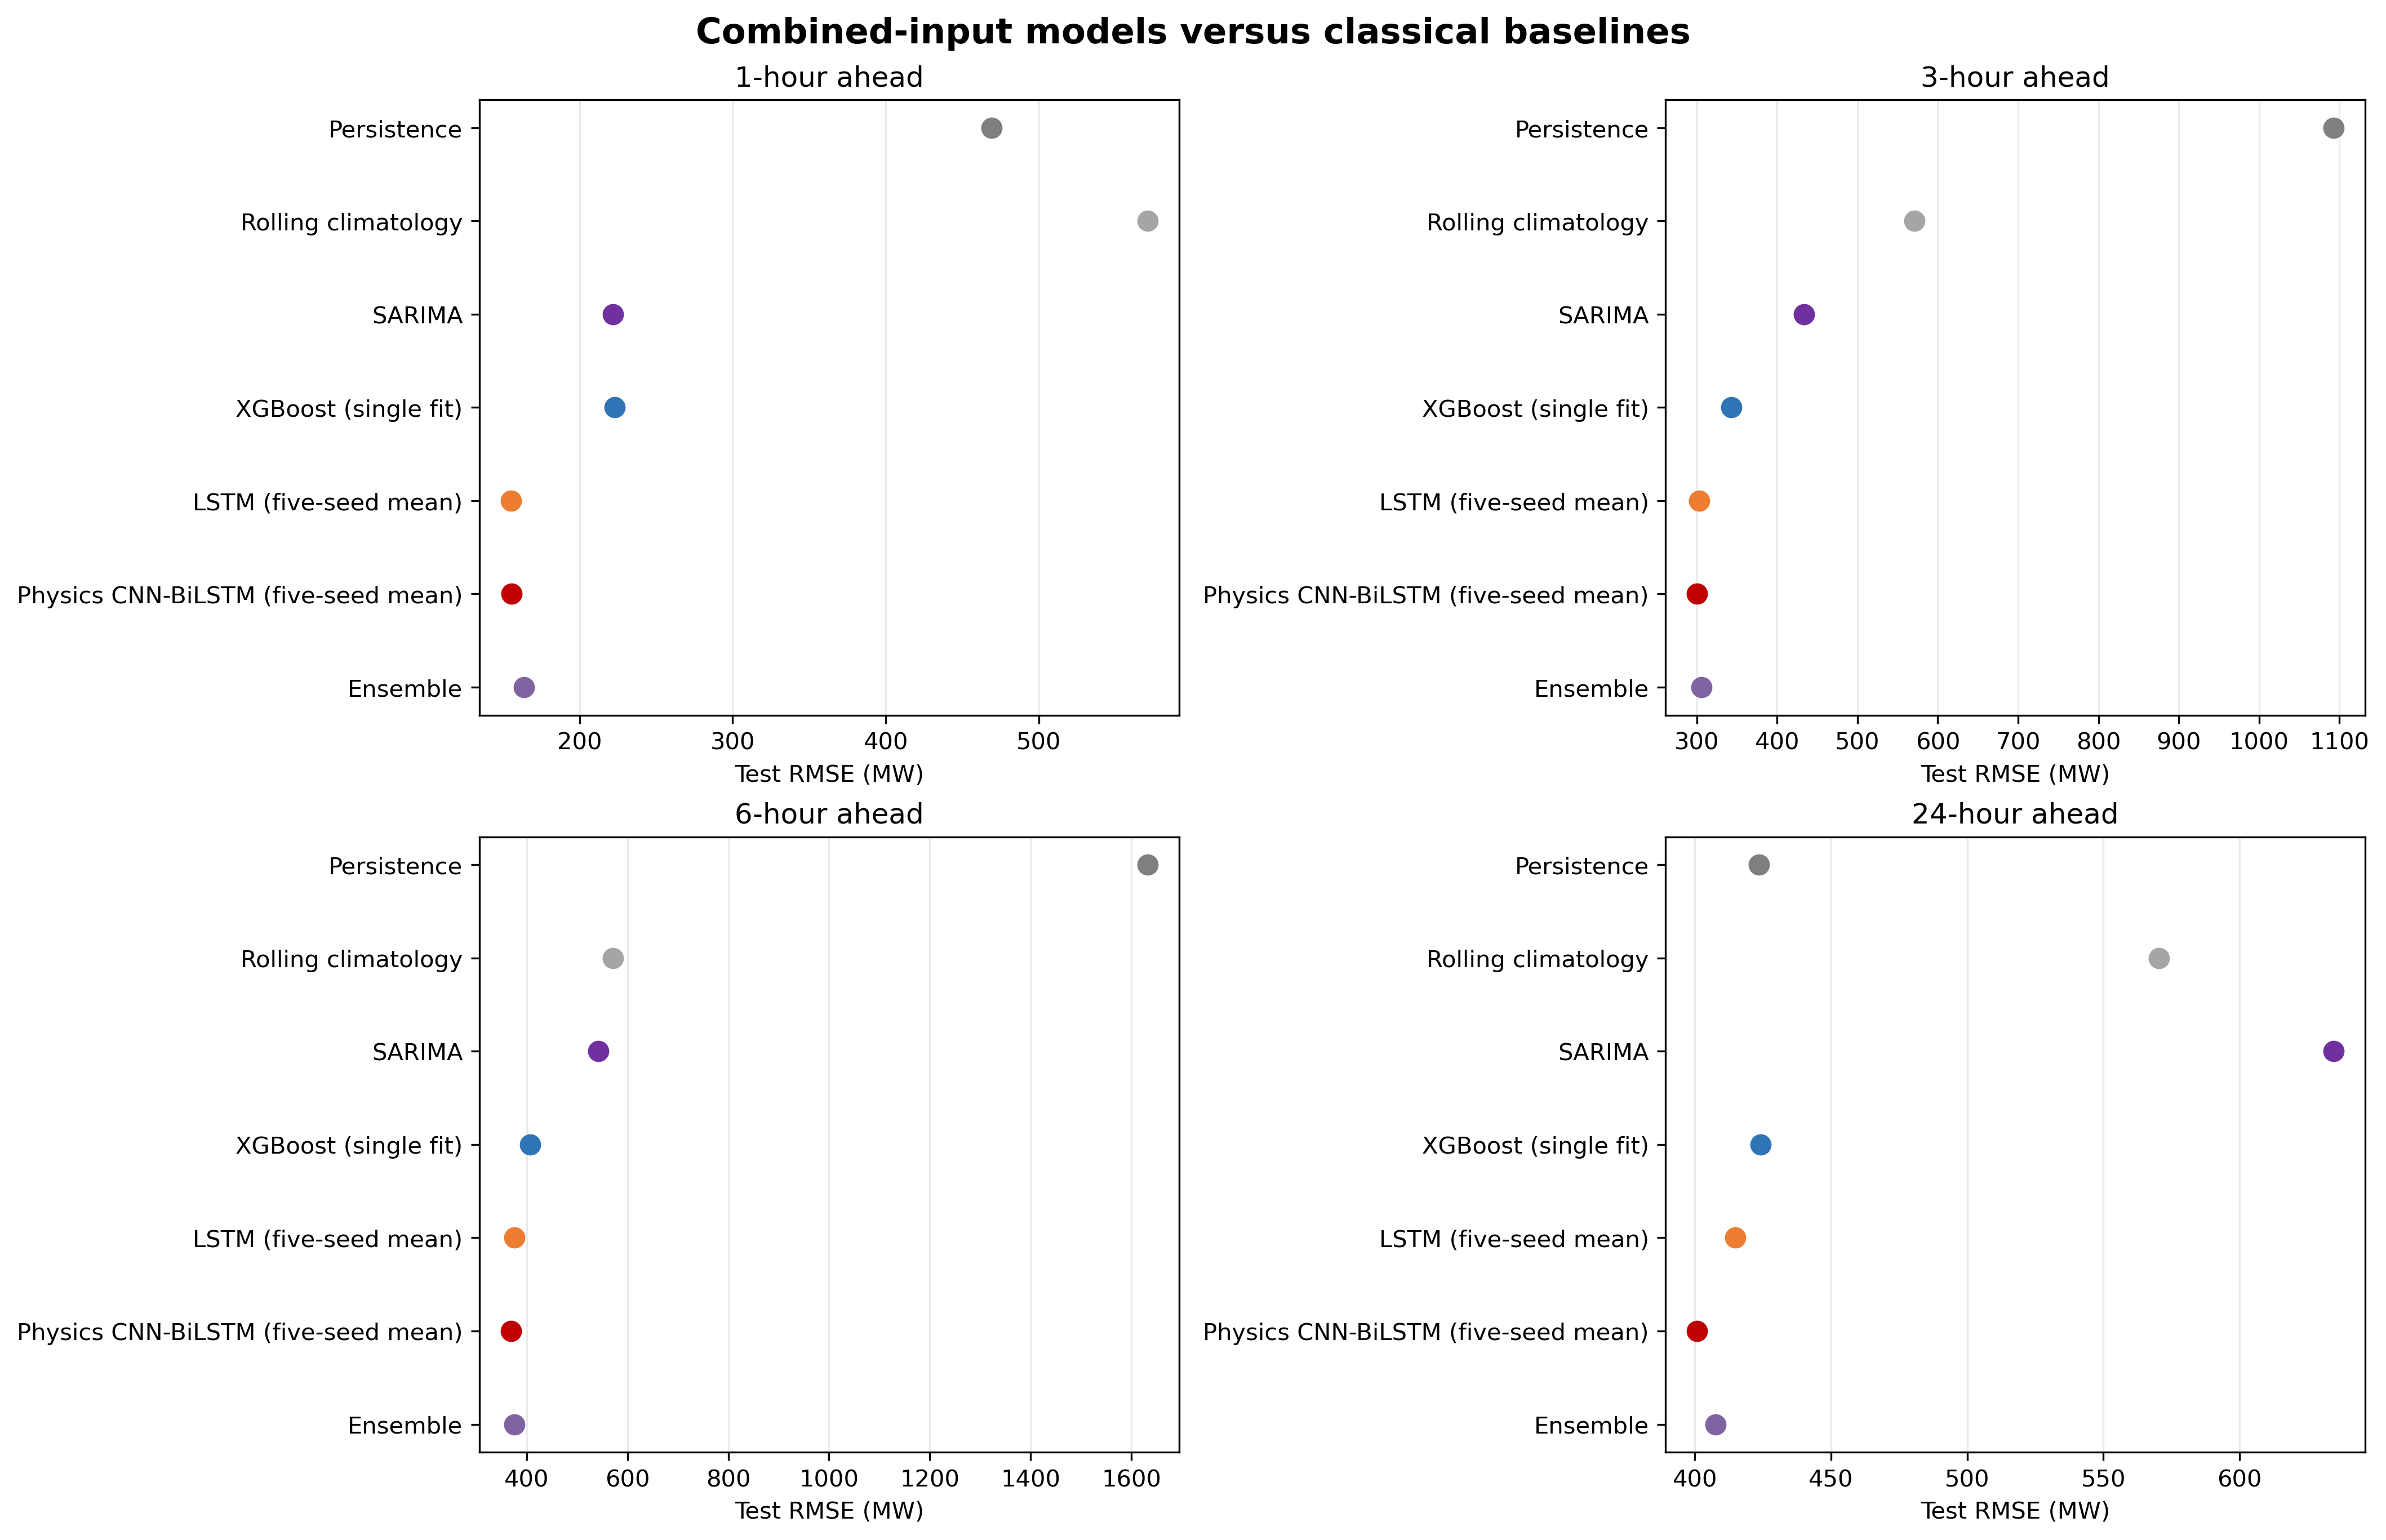
\includegraphics[width=\linewidth,height=0.46\textheight,keepaspectratio]{figures/baseline_comparison_rmse.png}
\caption[Baseline RMSE across forecast horizons.]{RMSE of persistence, rolling climatology and SARIMA across forecast horizons.}\label{fig:ch4_8}\end{figure}

\subsection{Learned-Model Performance}

On combined inputs, LSTM gives the lowest 1-hour RMSE, while the physics-guided CNN-\allowbreak{}BiLSTM is best at 3 and 6 hours. The unconstrained CNN-\allowbreak{}BiLSTM is best at 24 hours. XGBoost beats persistence substantially at 1-6 hours but not at 24 hours.

Absolute error grows with horizon for every learned model, but relative skill does not change monotonically. XGBoost RMSE increases from 230.70 to 410.07 MW between one and six hours, while its persistence skill rises from 50.82 to 74.87 percent because persistence deteriorates faster. At 24 hours learned RMSE spans 399.77 to 435.82 MW and persistence skill ranges from -2.88 to 5.63 percent.

\begingroup\setlength{\tabcolsep}{3.5pt}\renewcommand{\arraystretch}{1.1}
\newcolumntype{L}[1]{>{\raggedright\arraybackslash}p{#1\linewidth}}
\begin{longtable}{|L{0.15773}|L{0.04639}|L{0.10206}|L{0.11134}|L{0.10206}|L{0.11134}|L{0.07423}|L{0.11134}|L{0.08351}|}
\caption{Combined-input learned-model and ensemble metrics. RMSE, MAE, bias and daylight RMSE are MW.}\label{tab:ch4_2}\\
\hline
\textbf{Model} & \textbf{h} & \textbf{RMSE} & \textbf{Relative RMSE (\%)} & \textbf{MAE} & \textbf{Bias} & \textbf{R2} & \textbf{Daylight RMSE} & \textbf{Skill (\%)} \\ \hline
\endfirsthead
\multicolumn{9}{|l|}{\small Table 4.2 continued}\\ \hline
\textbf{Model} & \textbf{h} & \textbf{RMSE} & \textbf{Relative RMSE (\%)} & \textbf{MAE} & \textbf{Bias} & \textbf{R2} & \textbf{Daylight RMSE} & \textbf{Skill (\%)} \\ \hline
\endhead
\hline\endfoot
XGBoost & 1 & 230.70 & 6.88 & 119.82 & -69.47 & 0.96 & 329.57 & 50.82 \\ \hline
LSTM & 1 & 155.25 & 4.70 & 83.68 & -9.05 & 0.98 & 220.43 & 66.90 \\ \hline
CNN-\allowbreak{}BiLSTM & 1 & 155.58 & 4.71 & 85.98 & -16.53 & 0.98 & 221.50 & 66.83 \\ \hline
Physics-guided & 1 & 155.53 & 4.71 & 86.09 & -18.53 & 0.98 & 221.46 & 66.84 \\ \hline
Ensemble & 1 & 161.39 & 4.87 & 88.57 & -26.82 & 0.98 & 230.07 & 65.59 \\ \hline
XGBoost & 3 & 344.49 & 10.42 & 190.01 & -110.58 & 0.91 & 492.09 & 68.48 \\ \hline
LSTM & 3 & 302.65 & 9.16 & 165.90 & -52.09 & 0.93 & 430.89 & 72.30 \\ \hline
CNN-\allowbreak{}BiLSTM & 3 & 300.92 & 9.14 & 169.11 & -51.13 & 0.93 & 427.31 & 72.46 \\ \hline
Physics-guided & 3 & 300.28 & 9.12 & 170.12 & -50.85 & 0.93 & 426.52 & 72.52 \\ \hline
Ensemble & 3 & 303.88 & 9.21 & 169.34 & -65.49 & 0.93 & 432.94 & 72.19 \\ \hline
XGBoost & 6 & 410.07 & 12.43 & 228.15 & -148.87 & 0.88 & 585.83 & 74.87 \\ \hline
LSTM & 6 & 375.28 & 11.37 & 216.11 & -90.88 & 0.90 & 533.77 & 77.00 \\ \hline
CNN-\allowbreak{}BiLSTM & 6 & 373.57 & 11.34 & 218.92 & -85.29 & 0.90 & 529.89 & 77.11 \\ \hline
Physics-guided & 6 & 369.17 & 11.20 & 217.28 & -78.09 & 0.90 & 523.53 & 77.38 \\ \hline
Ensemble & 6 & 373.77 & 11.33 & 215.43 & -100.16 & 0.90 & 532.19 & 77.10 \\ \hline
XGBoost & 24 & 435.82 & 13.20 & 248.83 & -132.44 & 0.86 & 622.48 & -2.88 \\ \hline
LSTM & 24 & 414.86 & 12.59 & 239.90 & -121.68 & 0.87 & 591.80 & 2.06 \\ \hline
CNN-\allowbreak{}BiLSTM & 24 & 399.77 & 12.16 & 232.06 & -93.88 & 0.88 & 569.90 & 5.63 \\ \hline
Physics-guided & 24 & 400.81 & 12.19 & 231.78 & -95.44 & 0.88 & 571.66 & 5.38 \\ \hline
Ensemble & 24 & 407.40 & 12.37 & 235.35 & -110.52 & 0.88 & 581.59 & 3.83 \\ \hline
\end{longtable}\endgroup

\begin{figure}[!htbp]\centering
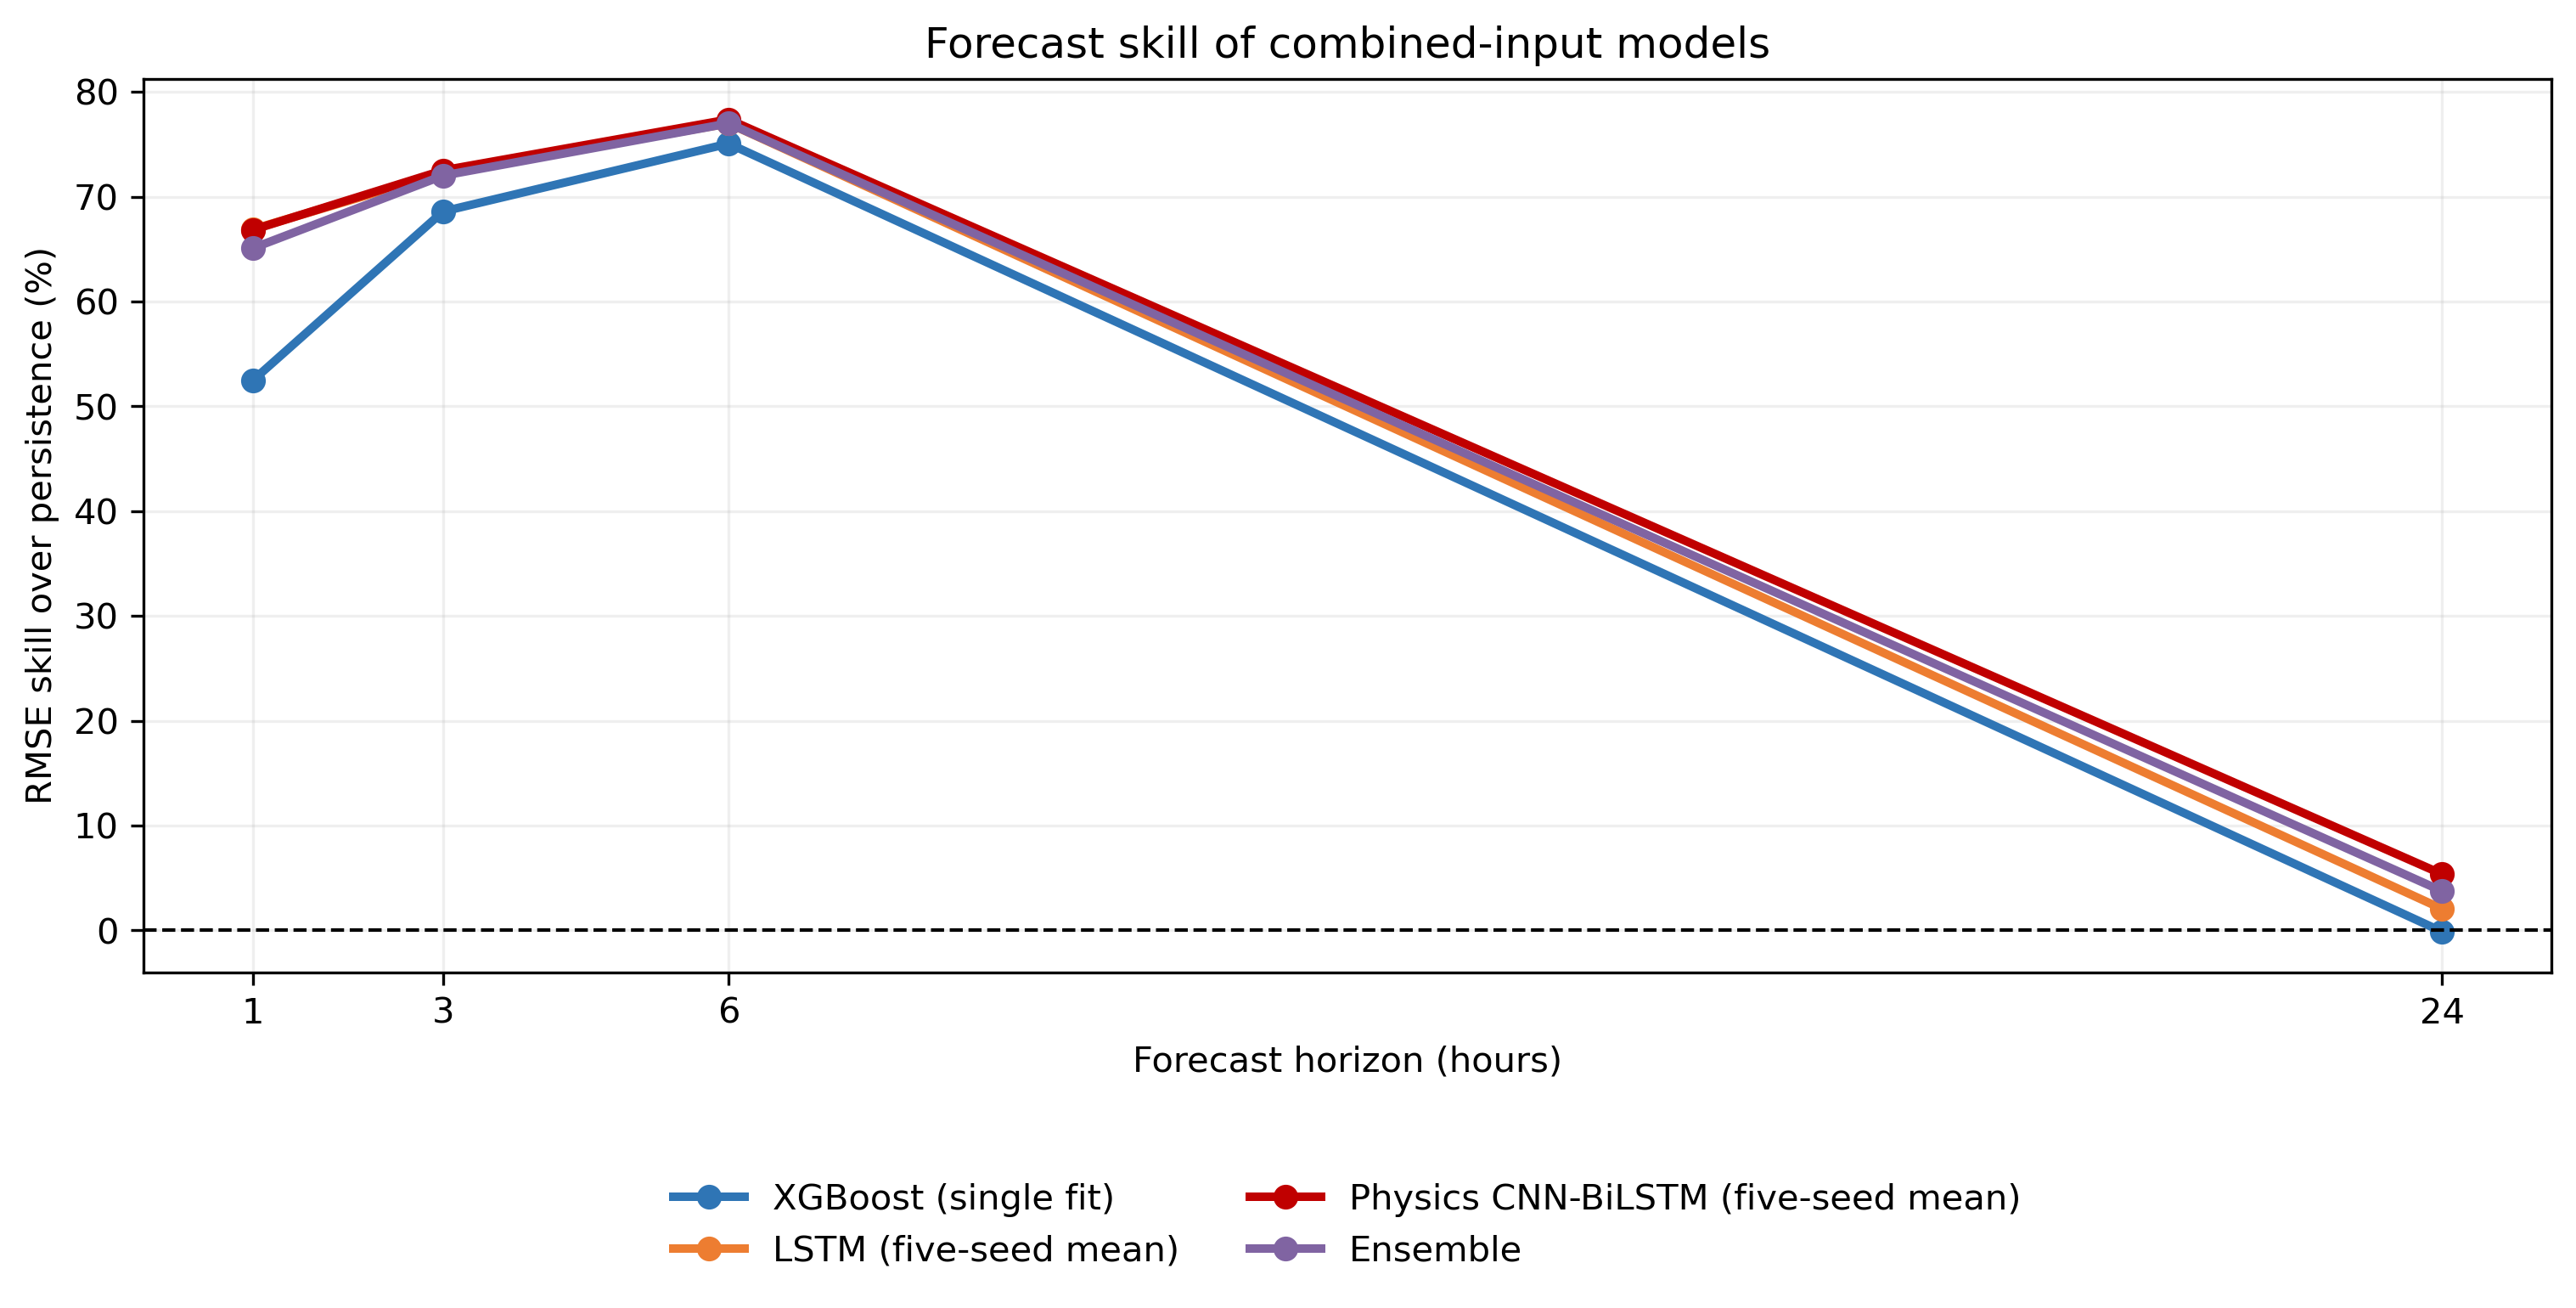
\includegraphics[width=\linewidth,height=0.46\textheight,keepaspectratio]{figures/forecast_skill_by_model.png}
\caption[Persistence skill of learned models and ensemble.]{Persistence skill of learned models and the descriptive ensemble on combined inputs.}\label{fig:ch4_9}\end{figure}

\begin{figure}[!htbp]\centering
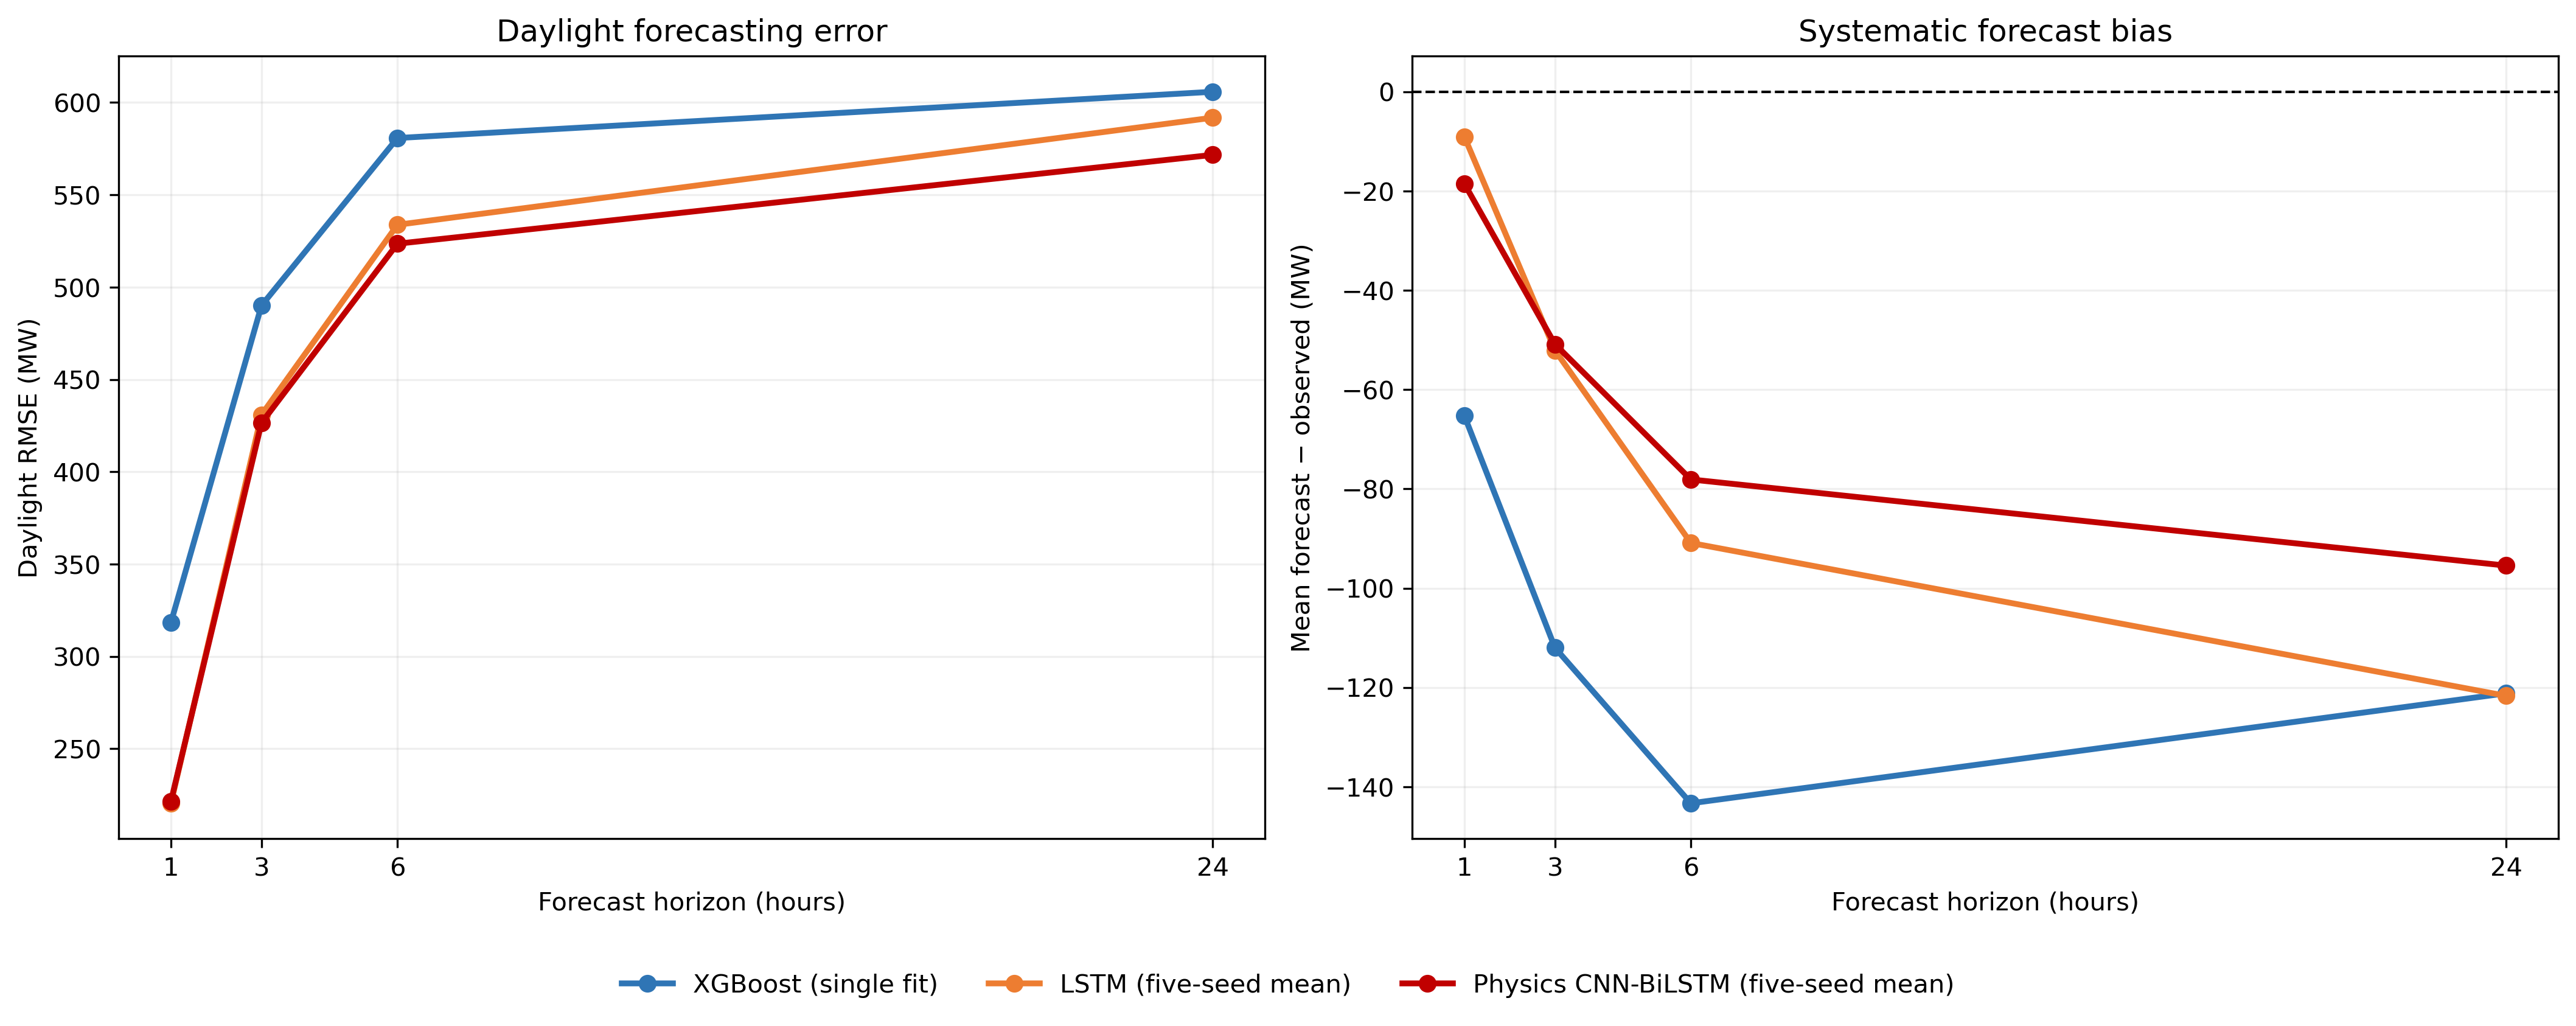
\includegraphics[width=\linewidth,height=0.46\textheight,keepaspectratio]{figures/learned_model_error_diagnostics.png}
\caption[Daylight error and signed bias by horizon.]{Daylight error and signed bias by horizon for three selected learned procedures. Bias grows steadily with horizon, which the aggregate RMSE alone does not show.}\label{fig:ch4_10}\end{figure}

The additional metrics agree with the RMSE ordering. Bias is negative for every configuration and largest for XGBoost at each horizon. Daylight RMSE exceeds all-hour RMSE because retained night-time zeros are easy, so no scalar score represents uniform performance across the operating day.

Zero clipping also forms part of the measurement chain. At one hour, 16.71 percent of LSTM and physics-guided, 19.47 percent of CNN-\allowbreak{}BiLSTM and 8.38 percent of XGBoost outputs are clipped. Much clipping falls at night, where zero is appropriate, but it can mask an unconstrained negative prediction.

The ranking must be qualified by paired inference. All neural procedures robustly outperform XGBoost at 1, 3 and 6 hours. Both CNN-\allowbreak{}BiLSTM variants also do so at 24 hours, while LSTM does not after correction. Among neural procedures, the two CNN-\allowbreak{}BiLSTM variants outperform LSTM robustly only at 24 hours.

The matched comparison isolates the physical penalties. Their point gain is 0.04 percent at 1 hour, 0.21 at 3 hours, 1.18 at 6 hours and -0.26 at 24 hours. Only the 6-hour gain is robust; the other horizons do not establish a penalty benefit or harm.

\begin{figure}[!htbp]\centering
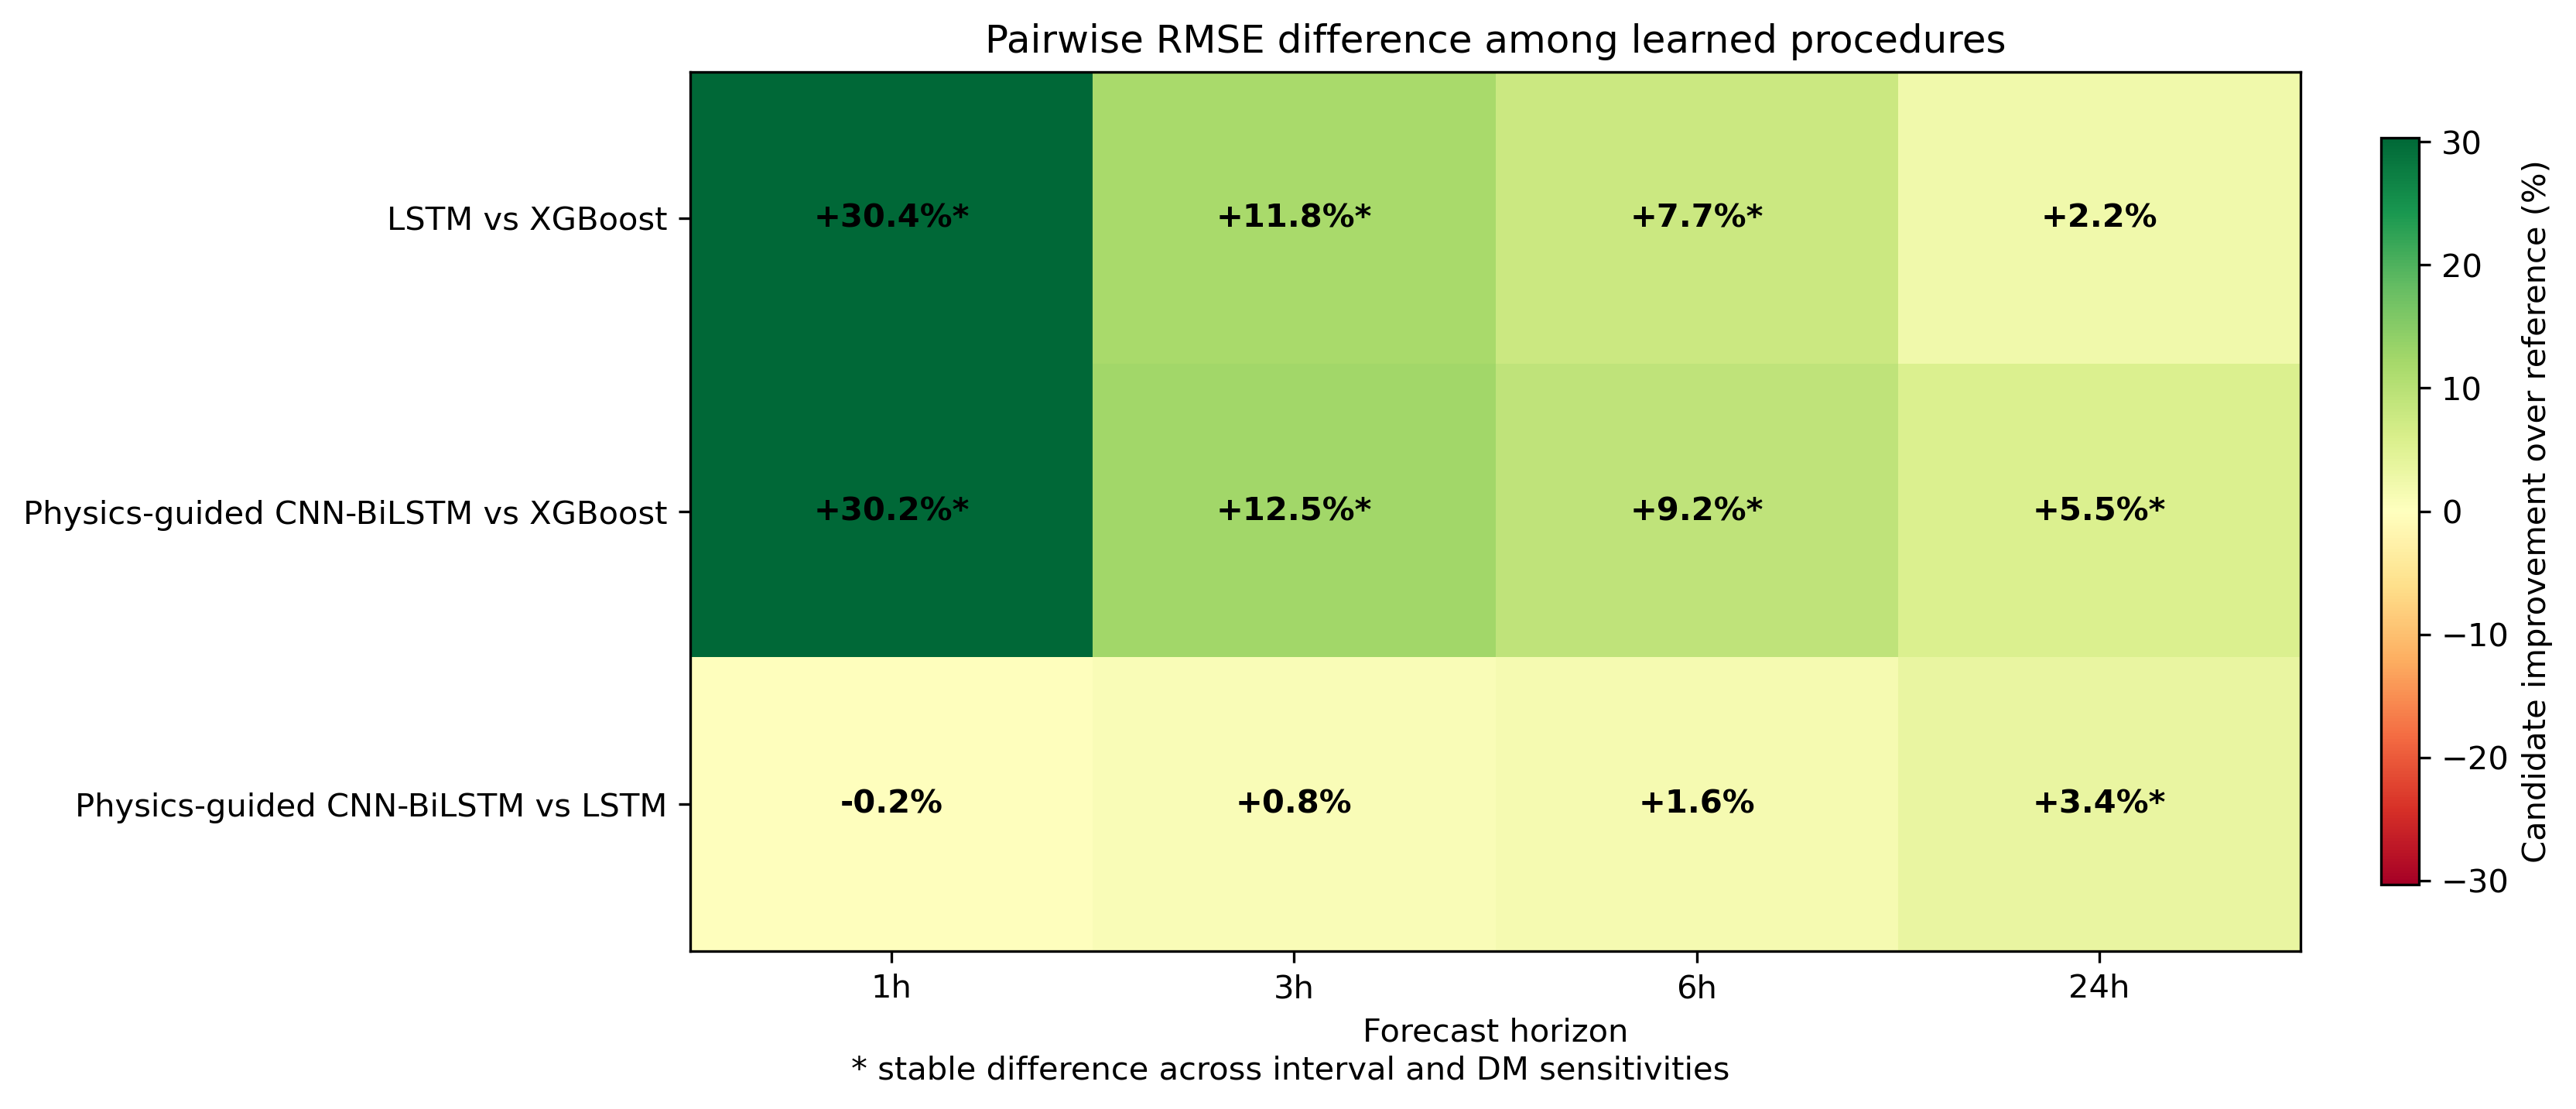
\includegraphics[width=\linewidth,height=0.46\textheight,keepaspectratio]{figures/pairwise_model_superiority.png}
\caption[Pairwise RMSE comparison of learned procedures.]{Dependence-robust pairwise conclusions among learned models.}\label{fig:ch4_11}\end{figure}

\begingroup\setlength{\tabcolsep}{3.5pt}\renewcommand{\arraystretch}{1.1}
\newcolumntype{L}[1]{>{\raggedright\arraybackslash}p{#1\linewidth}}
\begin{longtable}{|L{0.27000}|L{0.08100}|L{0.18000}|L{0.36900}|}
\caption{Pairwise learned-model RMSE gain of the second model over the first and robust conclusion.}\label{tab:ch4_3}\\
\hline
\textbf{Comparison} & \textbf{h} & \textbf{Gain (\%)} & \textbf{Robust conclusion} \\ \hline
\endfirsthead
\multicolumn{4}{|l|}{\small Table 4.3 continued}\\ \hline
\textbf{Comparison} & \textbf{h} & \textbf{Gain (\%)} & \textbf{Robust conclusion} \\ \hline
\endhead
\hline\endfoot
XGBoost vs LSTM & 1 & 32.71 & LSTM better \\ \hline
XGBoost vs LSTM & 3 & 12.15 & LSTM better \\ \hline
XGBoost vs LSTM & 6 & 8.49 & LSTM better \\ \hline
XGBoost vs LSTM & 24 & 4.81 & No robust difference \\ \hline
XGBoost vs CNN-\allowbreak{}BiLSTM & 1 & 32.56 & CNN-\allowbreak{}BiLSTM better \\ \hline
XGBoost vs CNN-\allowbreak{}BiLSTM & 3 & 12.65 & CNN-\allowbreak{}BiLSTM better \\ \hline
XGBoost vs CNN-\allowbreak{}BiLSTM & 6 & 8.90 & CNN-\allowbreak{}BiLSTM better \\ \hline
XGBoost vs CNN-\allowbreak{}BiLSTM & 24 & 8.27 & CNN-\allowbreak{}BiLSTM better \\ \hline
XGBoost vs Physics-guided & 1 & 32.58 & Physics-guided better \\ \hline
XGBoost vs Physics-guided & 3 & 12.83 & Physics-guided better \\ \hline
XGBoost vs Physics-guided & 6 & 9.98 & Physics-guided better \\ \hline
XGBoost vs Physics-guided & 24 & 8.03 & Physics-guided better \\ \hline
LSTM vs CNN-\allowbreak{}BiLSTM & 1 & -0.22 & No robust difference \\ \hline
LSTM vs CNN-\allowbreak{}BiLSTM & 3 & 0.57 & No robust difference \\ \hline
LSTM vs CNN-\allowbreak{}BiLSTM & 6 & 0.46 & No robust difference \\ \hline
LSTM vs CNN-\allowbreak{}BiLSTM & 24 & 3.64 & CNN-\allowbreak{}BiLSTM better \\ \hline
LSTM vs Physics-guided & 1 & -0.18 & No robust difference \\ \hline
LSTM vs Physics-guided & 3 & 0.78 & No robust difference \\ \hline
LSTM vs Physics-guided & 6 & 1.63 & No robust difference \\ \hline
LSTM vs Physics-guided & 24 & 3.39 & Physics-guided better \\ \hline
CNN-\allowbreak{}BiLSTM vs Physics-guided & 1 & 0.04 & No robust difference \\ \hline
CNN-\allowbreak{}BiLSTM vs Physics-guided & 3 & 0.21 & No robust difference \\ \hline
CNN-\allowbreak{}BiLSTM vs Physics-guided & 6 & 1.18 & Physics-guided better \\ \hline
CNN-\allowbreak{}BiLSTM vs Physics-guided & 24 & -0.26 & No robust difference \\ \hline
\end{longtable}\endgroup

A separate finding concerns optimisation rather than information: the epoch minimising validation error falls sharply as the horizon lengthens, and the day-ahead fits stop improving well before the intraday fits.

\begingroup\setlength{\tabcolsep}{3.5pt}\renewcommand{\arraystretch}{1.1}
\newcolumntype{L}[1]{>{\raggedright\arraybackslash}p{#1\linewidth}}
\begin{longtable}{|L{0.22500}|L{0.16200}|L{0.11700}|L{0.13500}|L{0.12600}|L{0.13500}|}
\caption{Mean best-validation epoch across the five seeds, by model, feature set and horizon. Lower values mean the fit stopped improving sooner.}\label{tab:ch4_4}\\
\hline
\textbf{Model} & \textbf{Inputs} & \textbf{1h} & \textbf{3h} & \textbf{6h} & \textbf{24h} \\ \hline
\endfirsthead
\multicolumn{6}{|l|}{\small Table 4.4 continued}\\ \hline
\textbf{Model} & \textbf{Inputs} & \textbf{1h} & \textbf{3h} & \textbf{6h} & \textbf{24h} \\ \hline
\endhead
\hline\endfoot
LSTM & combined & 61.2 & 31.0 & 18.4 & 8.8 \\ \hline
LSTM & weather\_\allowbreak{}history & 51.2 & 39.2 & 20.2 & 11.6 \\ \hline
CNN-\allowbreak{}BiLSTM & combined & 54.8 & 23.8 & 22.6 & 12.0 \\ \hline
CNN-\allowbreak{}BiLSTM & weather\_\allowbreak{}history & 63.4 & 22.0 & 22.8 & 12.0 \\ \hline
Physics-guided CNN-\allowbreak{}BiLSTM & combined & 62.0 & 23.4 & 21.6 & 12.4 \\ \hline
Physics-guided CNN-\allowbreak{}BiLSTM & weather\_\allowbreak{}history & 60.0 & 26.2 & 22.4 & 12.0 \\ \hline
\end{longtable}\endgroup

The one-hour history-based fits improve for roughly 51 to 63 epochs, whereas the day-ahead fits stop improving within about 9 to 12 epochs. This concerns optimisation under the fixed schedule, not the information content of the inputs.

\subsection{Controlled Contribution of Intra-Hour Features}

Without ordinary history, the two scale-normalised summaries improve every learned procedure at every horizon under the full decision rule. Gains range from 1.26 to 11.46 percent. Agreement across four different procedures, weekly-block intervals, corrected tests and the output-scale sensitivity strengthens the conclusion that the summaries carry predictive information beyond retrospective meteorology alone.

\begingroup\setlength{\tabcolsep}{3.5pt}\renewcommand{\arraystretch}{1.1}
\newcolumntype{L}[1]{>{\raggedright\arraybackslash}p{#1\linewidth}}
\begin{longtable}{|L{0.12857}|L{0.12857}|L{0.12857}|L{0.12857}|L{0.12857}|L{0.12857}|L{0.12857}|}
\caption{Intra-hour contribution without hourly history. Positive gain favours weather\_\allowbreak{}intra; confidence intervals use 168-hour blocks.}\label{tab:ch4_5}\\
\hline
\textbf{Model} & \textbf{h} & \textbf{RMSE weather} & \textbf{RMSE weather\_\allowbreak{}intra} & \textbf{Gain (\%)} & \textbf{95\% CI (\%)} & \textbf{Scale gain (\%)} \\ \hline
\endfirsthead
\multicolumn{7}{|l|}{\small Table 4.5 continued}\\ \hline
\textbf{Model} & \textbf{h} & \textbf{RMSE weather} & \textbf{RMSE weather\_\allowbreak{}intra} & \textbf{Gain (\%)} & \textbf{95\% CI (\%)} & \textbf{Scale gain (\%)} \\ \hline
\endhead
\hline\endfoot
XGBoost & 1 & 722.73 & 690.18 & 4.50 & 3.15 to 6.13 & 4.68 \\ \hline
XGBoost & 3 & 729.24 & 707.76 & 2.95 & 1.94 to 4.10 & 3.08 \\ \hline
XGBoost & 6 & 730.86 & 714.90 & 2.18 & 1.29 to 3.19 & 2.31 \\ \hline
XGBoost & 24 & 746.36 & 736.95 & 1.26 & 0.67 to 1.91 & 1.31 \\ \hline
LSTM & 1 & 695.51 & 615.80 & 11.46 & 8.62 to 14.11 & 11.32 \\ \hline
LSTM & 3 & 690.91 & 635.16 & 8.07 & 6.12 to 9.95 & 8.16 \\ \hline
LSTM & 6 & 695.79 & 653.63 & 6.06 & 3.80 to 8.37 & 6.07 \\ \hline
LSTM & 24 & 722.51 & 664.96 & 7.97 & 5.52 to 10.33 & 7.86 \\ \hline
CNN-\allowbreak{}BiLSTM & 1 & 674.77 & 615.90 & 8.72 & 6.61 to 11.09 & 8.81 \\ \hline
CNN-\allowbreak{}BiLSTM & 3 & 687.31 & 642.52 & 6.52 & 5.04 to 8.18 & 6.56 \\ \hline
CNN-\allowbreak{}BiLSTM & 6 & 690.28 & 651.55 & 5.61 & 4.18 to 7.00 & 5.62 \\ \hline
CNN-\allowbreak{}BiLSTM & 24 & 708.47 & 651.34 & 8.06 & 6.63 to 9.66 & 8.24 \\ \hline
Physics-guided & 1 & 677.33 & 608.46 & 10.17 & 7.89 to 12.62 & 10.19 \\ \hline
Physics-guided & 3 & 687.92 & 635.70 & 7.59 & 6.03 to 9.48 & 7.79 \\ \hline
Physics-guided & 6 & 693.15 & 650.90 & 6.09 & 4.59 to 7.67 & 6.14 \\ \hline
Physics-guided & 24 & 704.86 & 652.50 & 7.43 & 5.64 to 9.10 & 7.40 \\ \hline
\end{longtable}\endgroup

The research-question contrast is more selective after hourly history is controlled. All four procedures improve robustly at 1 hour. XGBoost and the physics-guided procedure also improve robustly at 3 and 6 hours. The remaining intraday cells are inconclusive, and no procedure establishes a robust 24-hour benefit.

\begingroup\setlength{\tabcolsep}{3.5pt}\renewcommand{\arraystretch}{1.1}
\newcolumntype{L}[1]{>{\raggedright\arraybackslash}p{#1\linewidth}}
\begin{longtable}{|L{0.10800}|L{0.04500}|L{0.11700}|L{0.12600}|L{0.09000}|L{0.11700}|L{0.10800}|L{0.18900}|}
\caption{Controlled intra-hour contribution relative to weather\_\allowbreak{}history. Positive gain favours combined; confidence intervals use 168-hour blocks.}\label{tab:ch4_6}\\
\hline
\textbf{Model} & \textbf{h} & \textbf{RMSE history} & \textbf{RMSE combined} & \textbf{Gain (\%)} & \textbf{95\% CI (\%)} & \textbf{Scale gain (\%)} & \textbf{Finding} \\ \hline
\endfirsthead
\multicolumn{8}{|l|}{\small Table 4.6 continued}\\ \hline
\textbf{Model} & \textbf{h} & \textbf{RMSE history} & \textbf{RMSE combined} & \textbf{Gain (\%)} & \textbf{95\% CI (\%)} & \textbf{Scale gain (\%)} & \textbf{Finding} \\ \hline
\endhead
\hline\endfoot
XGBoost & 1 & 235.17 & 230.70 & 1.90 & 1.06 to 2.91 & 2.08 & Robust improvement \\ \hline
XGBoost & 3 & 352.35 & 344.49 & 2.23 & 1.12 to 3.32 & 2.32 & Robust improvement \\ \hline
XGBoost & 6 & 422.14 & 410.07 & 2.86 & 1.92 to 3.80 & 2.97 & Robust improvement \\ \hline
XGBoost & 24 & 440.12 & 435.82 & 0.98 & 0.03 to 2.10 & 0.98 & Inconclusive \\ \hline
LSTM & 1 & 159.48 & 155.25 & 2.65 & 1.45 to 4.00 & 2.83 & Robust improvement \\ \hline
LSTM & 3 & 305.26 & 302.65 & 0.85 & -0.22 to 1.99 & 0.99 & Inconclusive \\ \hline
LSTM & 6 & 378.67 & 375.28 & 0.89 & 0.01 to 1.83 & 0.92 & Inconclusive \\ \hline
LSTM & 24 & 411.98 & 414.86 & -0.70 & -1.32 to 0.06 & -0.60 & Inconclusive \\ \hline
CNN-\allowbreak{}BiLSTM & 1 & 159.74 & 155.58 & 2.60 & 1.55 to 3.81 & 2.74 & Robust improvement \\ \hline
CNN-\allowbreak{}BiLSTM & 3 & 304.50 & 300.92 & 1.18 & 0.08 to 2.04 & 1.21 & Inconclusive \\ \hline
CNN-\allowbreak{}BiLSTM & 6 & 378.61 & 373.57 & 1.33 & 0.34 to 2.16 & 1.27 & Inconclusive \\ \hline
CNN-\allowbreak{}BiLSTM & 24 & 390.54 & 399.77 & -2.37 & -4.10 to -0.48 & -2.25 & Inconclusive \\ \hline
Physics-guided & 1 & 159.55 & 155.53 & 2.52 & 1.31 to 3.78 & 2.68 & Robust improvement \\ \hline
Physics-guided & 3 & 305.24 & 300.28 & 1.63 & 0.57 to 2.52 & 1.69 & Robust improvement \\ \hline
Physics-guided & 6 & 379.18 & 369.17 & 2.64 & 1.64 to 3.55 & 2.60 & Robust improvement \\ \hline
Physics-guided & 24 & 391.49 & 400.81 & -2.38 & -4.14 to -0.41 & -2.23 & Inconclusive \\ \hline
\end{longtable}\endgroup

Positive intervals alone do not determine the label. XGBoost at 24 hours and CNN-\allowbreak{}BiLSTM at 3 and 6 hours have intervals above zero, but at least one corrected dependence-sensitive test fails. The negative 24-hour intervals for both CNN-\allowbreak{}BiLSTM variants also remain inconclusive after family-wise correction.

\begin{figure}[!htbp]\centering
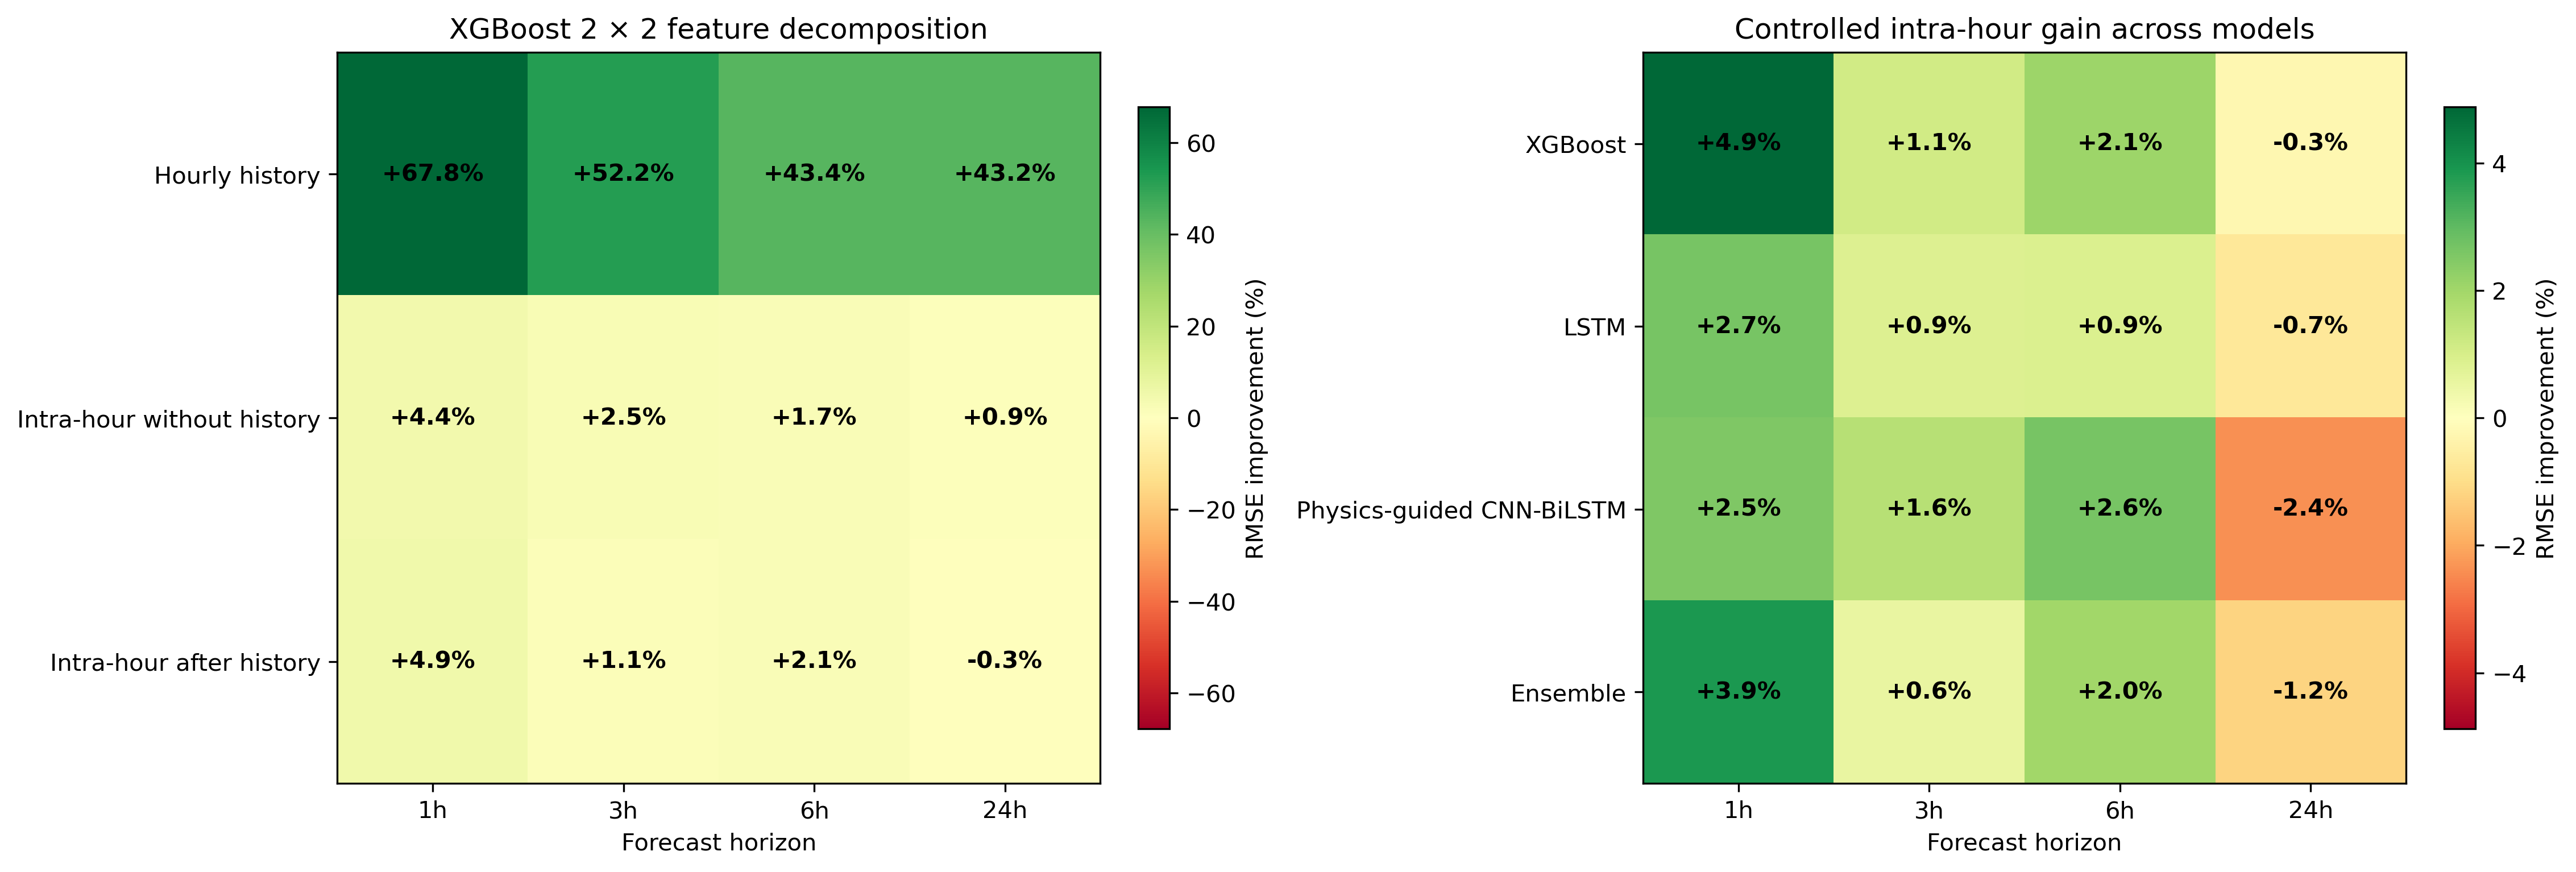
\includegraphics[width=\linewidth,height=0.46\textheight,keepaspectratio]{figures/feature_ablation_rmse.png}
\caption[RMSE across the four feature sets.]{RMSE under weather, hourly-history, intra-hour and combined feature sets.}\label{fig:ch4_12}\end{figure}

\begin{figure}[!htbp]\centering
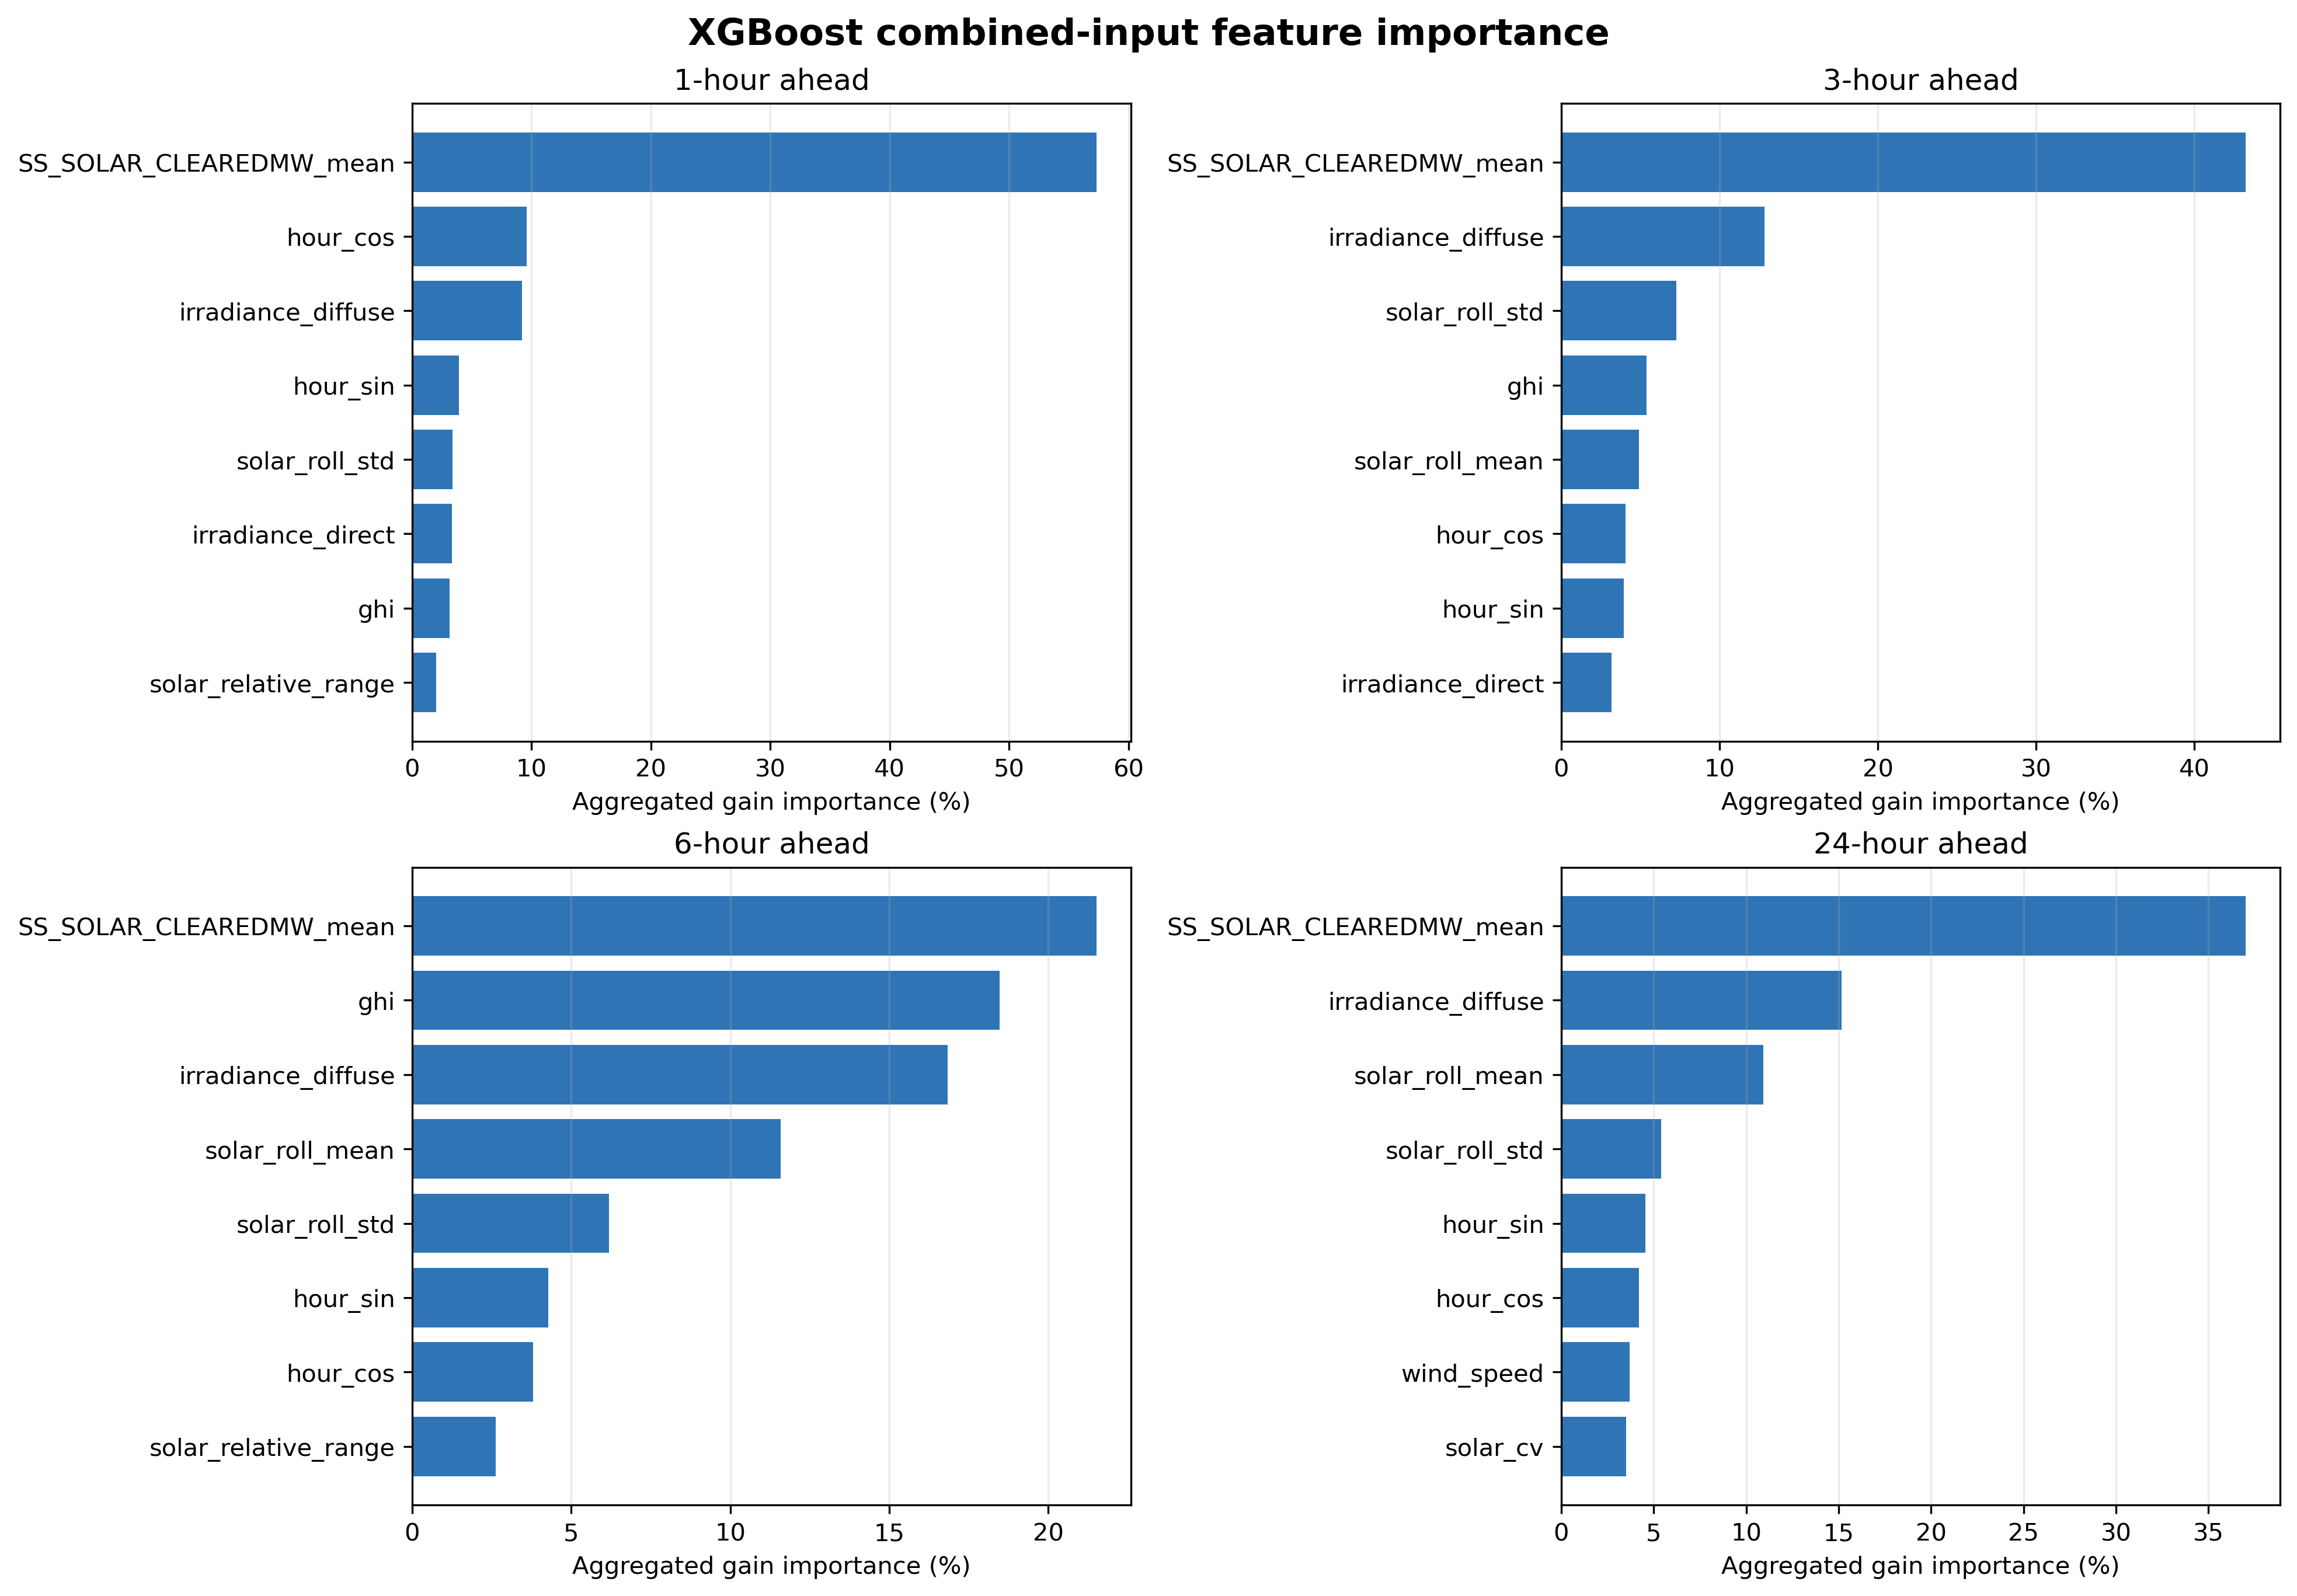
\includegraphics[width=\linewidth,height=0.46\textheight,keepaspectratio]{figures/xgboost_feature_importance.png}
\caption[XGBoost gain importance by lagged feature.]{Combined-input XGBoost gain importance aggregated across the 24 lag positions. A descriptive diagnostic of model use, not a causal attribution or a significance test.}\label{fig:ch4_13}\end{figure}

Ordinary hourly generation history is the larger effect, reducing meteorology-only RMSE by 41.03 to 77.07 percent, versus 1.26 to 11.46 percent for dispersion without history. Without history, every procedure benefits at every horizon. Once history is present, all four benefit robustly at 1 hour, only XGBoost and the physics-guided model do so at 3 and 6 hours, and none does at 24 hours. Neural 24-hour gains of 7.43 to 8.06 percent without history become changes of -0.70 to -2.38 percent with it, indicating redundancy. XGBoost settings are shared within each horizon and selected across all four arms, ruling out tuning on combined alone as the explanation.

\subsection{Baseline Robustness, Weather Regimes and Stability}

Across the 12 model-baseline comparisons for each learned procedure, XGBoost has 10 robust wins and each neural procedure has 11. All four learned procedures robustly outperform persistence at 1-6 hours but not at 24 hours, and all beat rolling climatology at every horizon. XGBoost does not robustly beat SARIMA at 1 hour; all neural procedures do.

The count of robust wins is a summary, not a league table: each 48-test bandwidth family includes references of different strength, and all horizons contribute equally.

\begin{figure}[!htbp]\centering
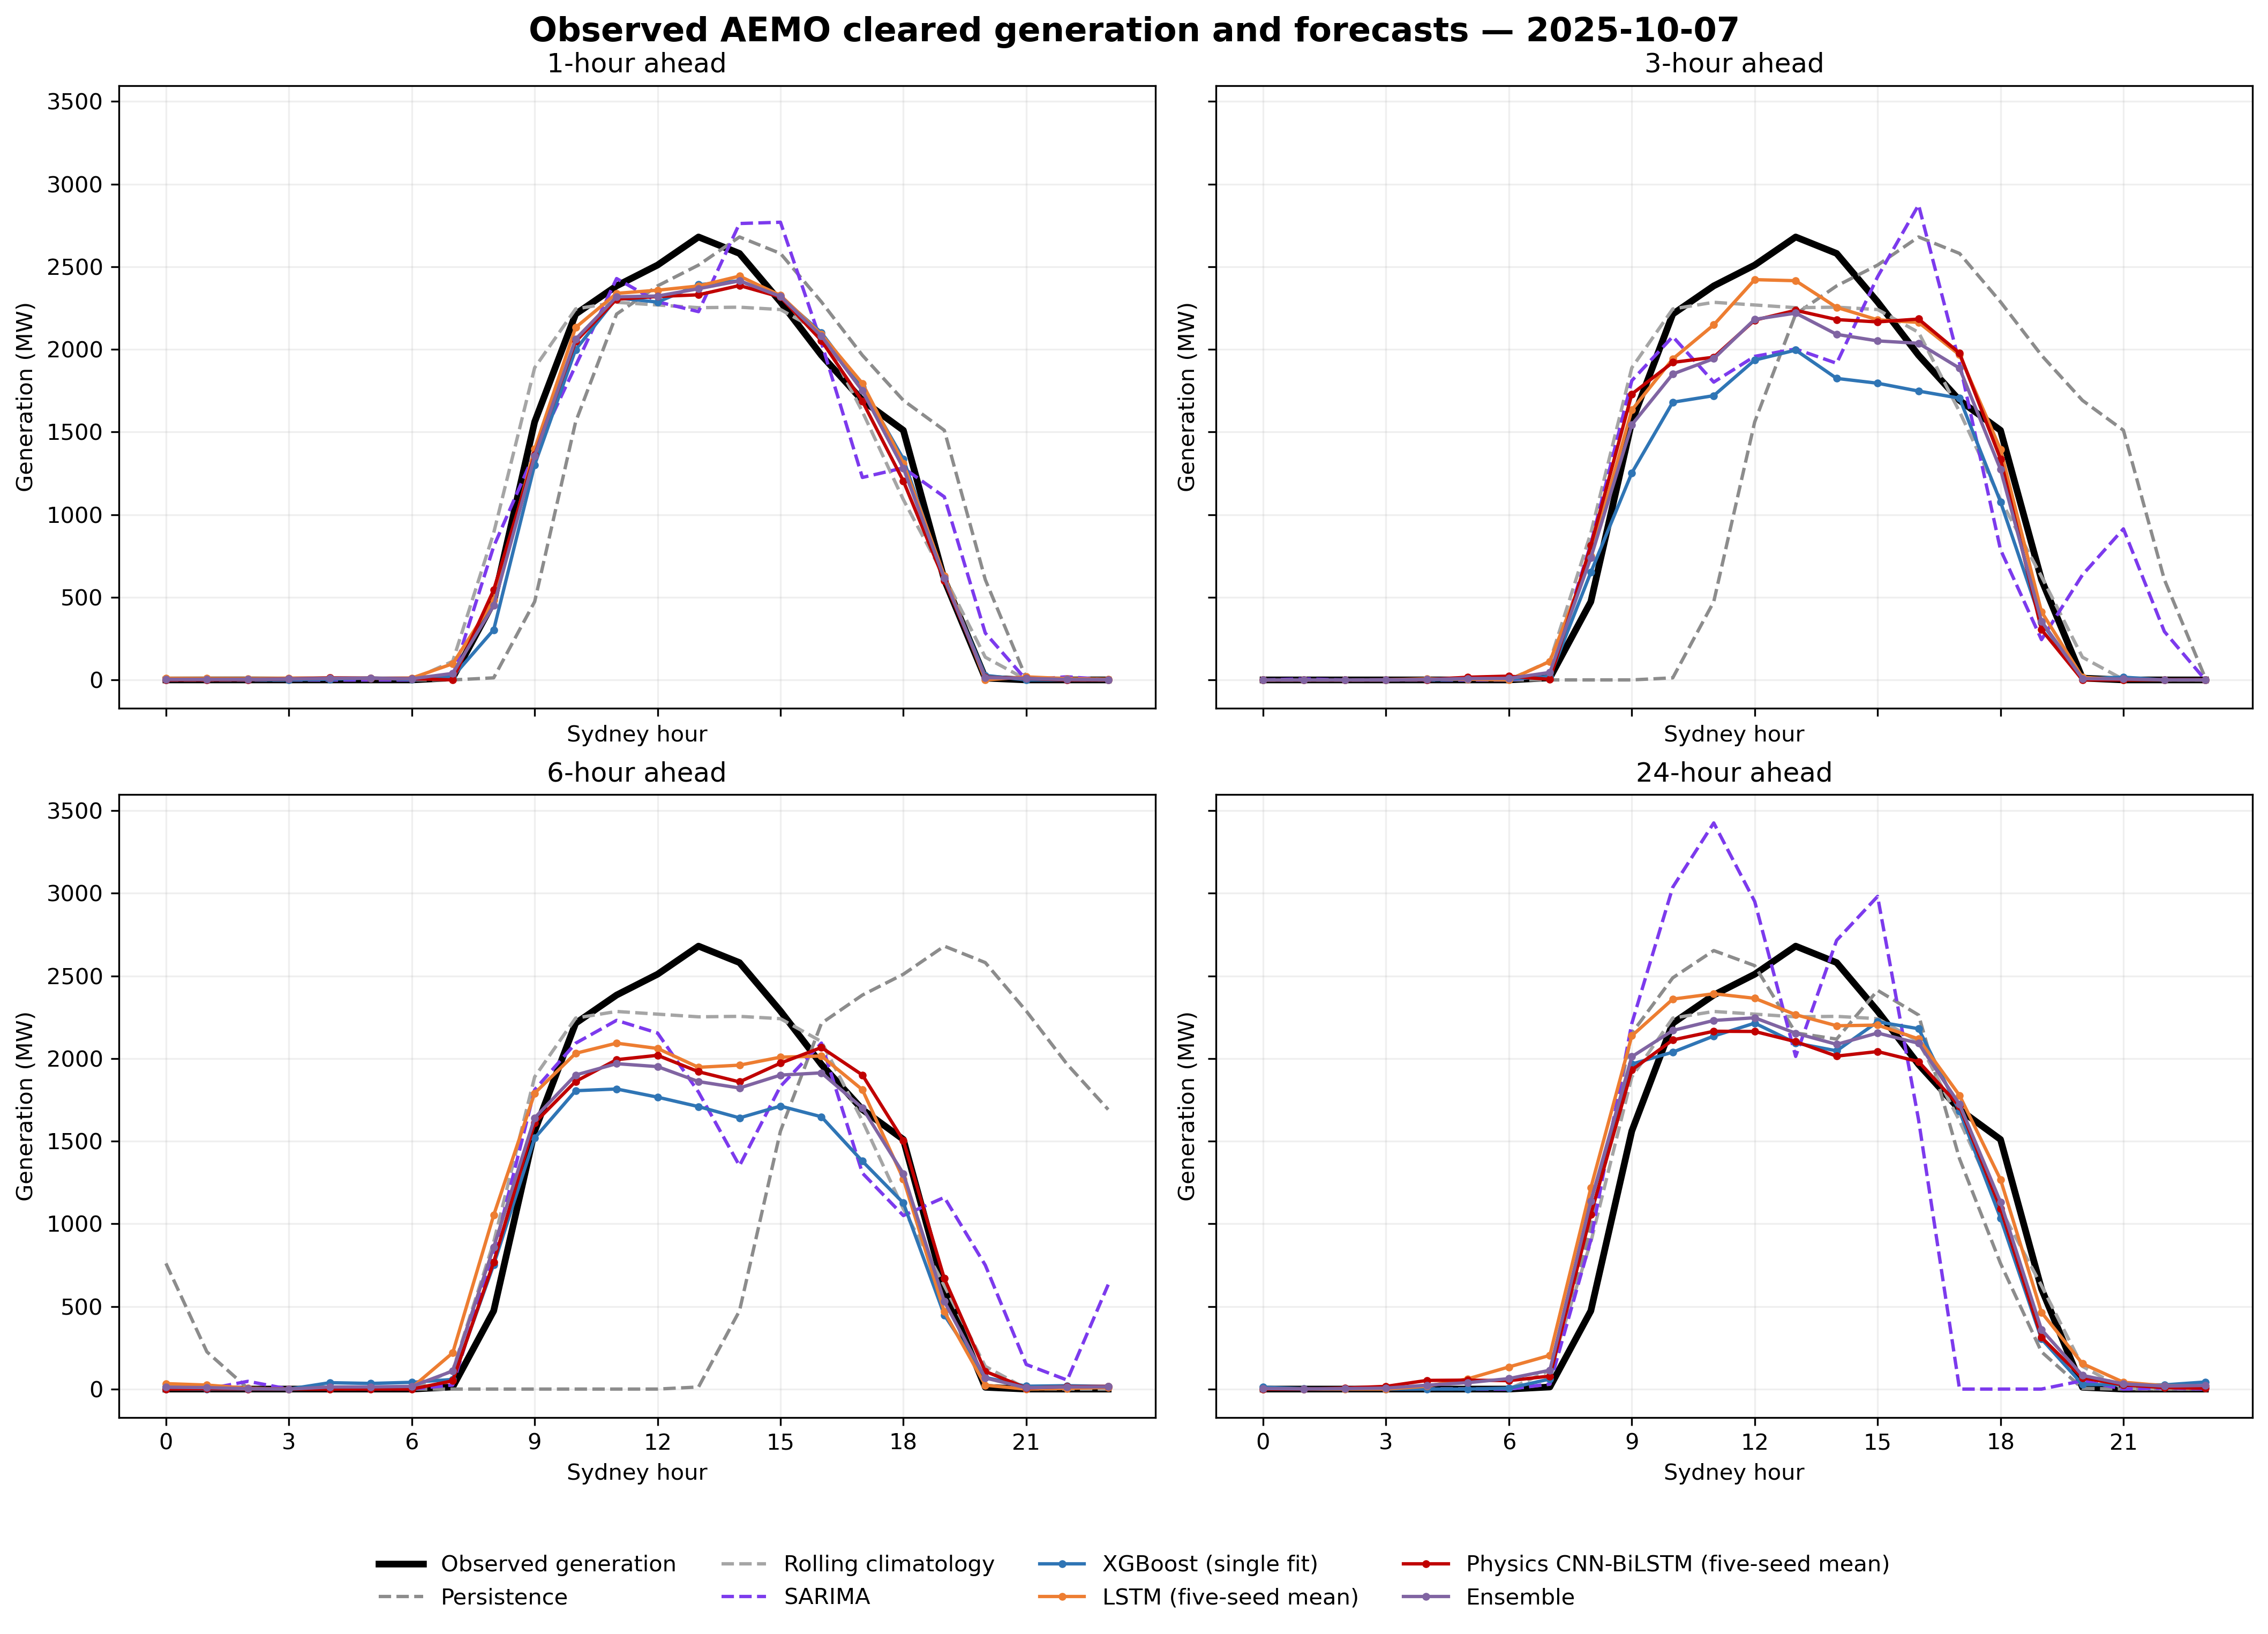
\includegraphics[width=\linewidth,height=0.46\textheight,keepaspectratio]{figures/all_models_observed_by_horizon.png}
\caption[Observed and forecast trajectories by horizon.]{Observed and forecast trajectories for all models by horizon.}\label{fig:ch4_14}\end{figure}

Weather-regime analysis shows that the controlled effect is not uniform. Table 4.7 uses target-time clearness index, which was not supplied to the models. The unequal strata contain 578 overcast hours (576 at 24 hours), 2,008 variable (2,000) and 1,688 clear (1,683). With no within-regime multiplicity correction or cell-level intervals, these repeated views of one test year are descriptive; negative cells are retained.

\begin{figure}[!htbp]\centering
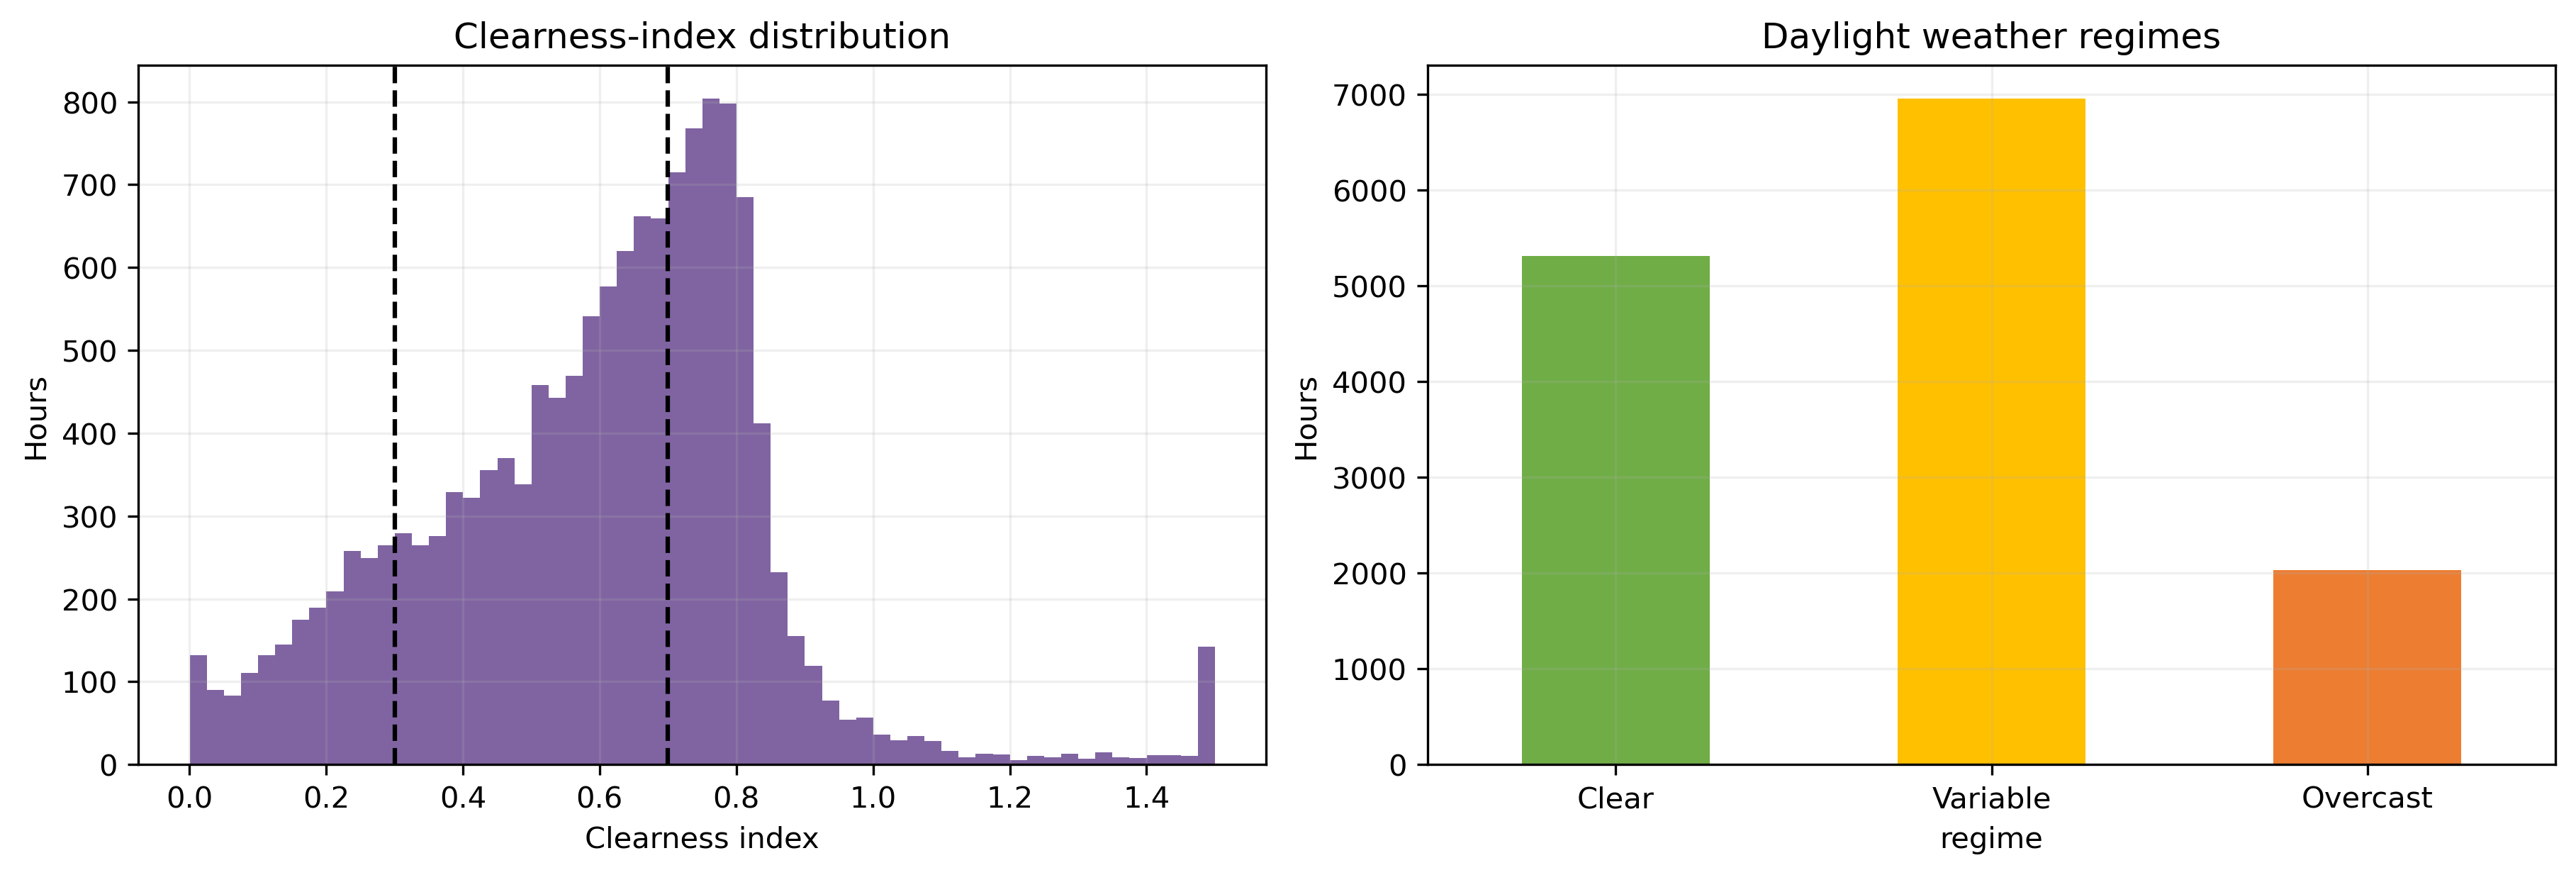
\includegraphics[width=\linewidth,height=0.46\textheight,keepaspectratio]{figures/clearness_index_regimes.png}
\caption[Clearness-index distribution and daylight weather regimes.]{Clearness-index distribution in daylight hours and the resulting overcast, variable and clear regime counts. The thresholds define the strata used in the regime analysis and are evaluation-only.}\label{fig:ch4_15}\end{figure}

\begingroup\setlength{\tabcolsep}{3.5pt}\renewcommand{\arraystretch}{1.1}
\newcolumntype{L}[1]{>{\raggedright\arraybackslash}p{#1\linewidth}}
\begin{longtable}{|L{0.22500}|L{0.16200}|L{0.11700}|L{0.13500}|L{0.12600}|L{0.13500}|}
\caption{Controlled intra-hour RMSE gain (\%) by daylight weather regime, from the predeclared weather\_\allowbreak{}history versus combined comparison.}\label{tab:ch4_7}\\
\hline
\textbf{Horizon} & \textbf{Overcast} & \textbf{Variable} & \textbf{Clear} & \textbf{Range} & \textbf{Negative cells} \\ \hline
\endfirsthead
\multicolumn{6}{|l|}{\small Table 4.7 continued}\\ \hline
\textbf{Horizon} & \textbf{Overcast} & \textbf{Variable} & \textbf{Clear} & \textbf{Range} & \textbf{Negative cells} \\ \hline
\endhead
\hline\endfoot
1h & +1.78 & +1.13 & +4.13 & -0.44 to +6.14 & 2 of 12 \\ \hline
3h & +2.02 & +1.08 & +1.66 & -1.62 to +3.53 & 2 of 12 \\ \hline
6h & -0.78 & +1.98 & +2.32 & -2.67 to +3.79 & 3 of 12 \\ \hline
24h & +0.83 & -0.67 & -1.99 & -3.94 to +3.85 & 8 of 12 \\ \hline
\end{longtable}\endgroup

Each cell is the mean across the four learned procedures, so the table summarises direction rather than any single model. The regime analysis remains descriptive and outside the confirmatory families.

The pattern contradicts the predeclared regime hypothesis, which expected the largest gain under variable cloud. Clear conditions rank highest at 1 and 6 hours, while variable conditions rank highest at no horizon. At 24 hours both variable and clear means are negative.

A second reading fits better. Under broken cloud the hourly mean already reflects the cloud-driven variation within it, so dispersion adds little beyond the level it is computed from; under clear skies that level is largely set by solar geometry, so residual dispersion still signals departure from it. The feature is thus most useful where hourly history is least informative alone, the opposite of what was predicted. The design cannot separate that account from the alternatives below: clearness-index thresholds are arbitrary, eight-site averaging smooths the spatial variation driving real cloud transitions, and regime counts are unequal.

\begin{figure}[!htbp]\centering
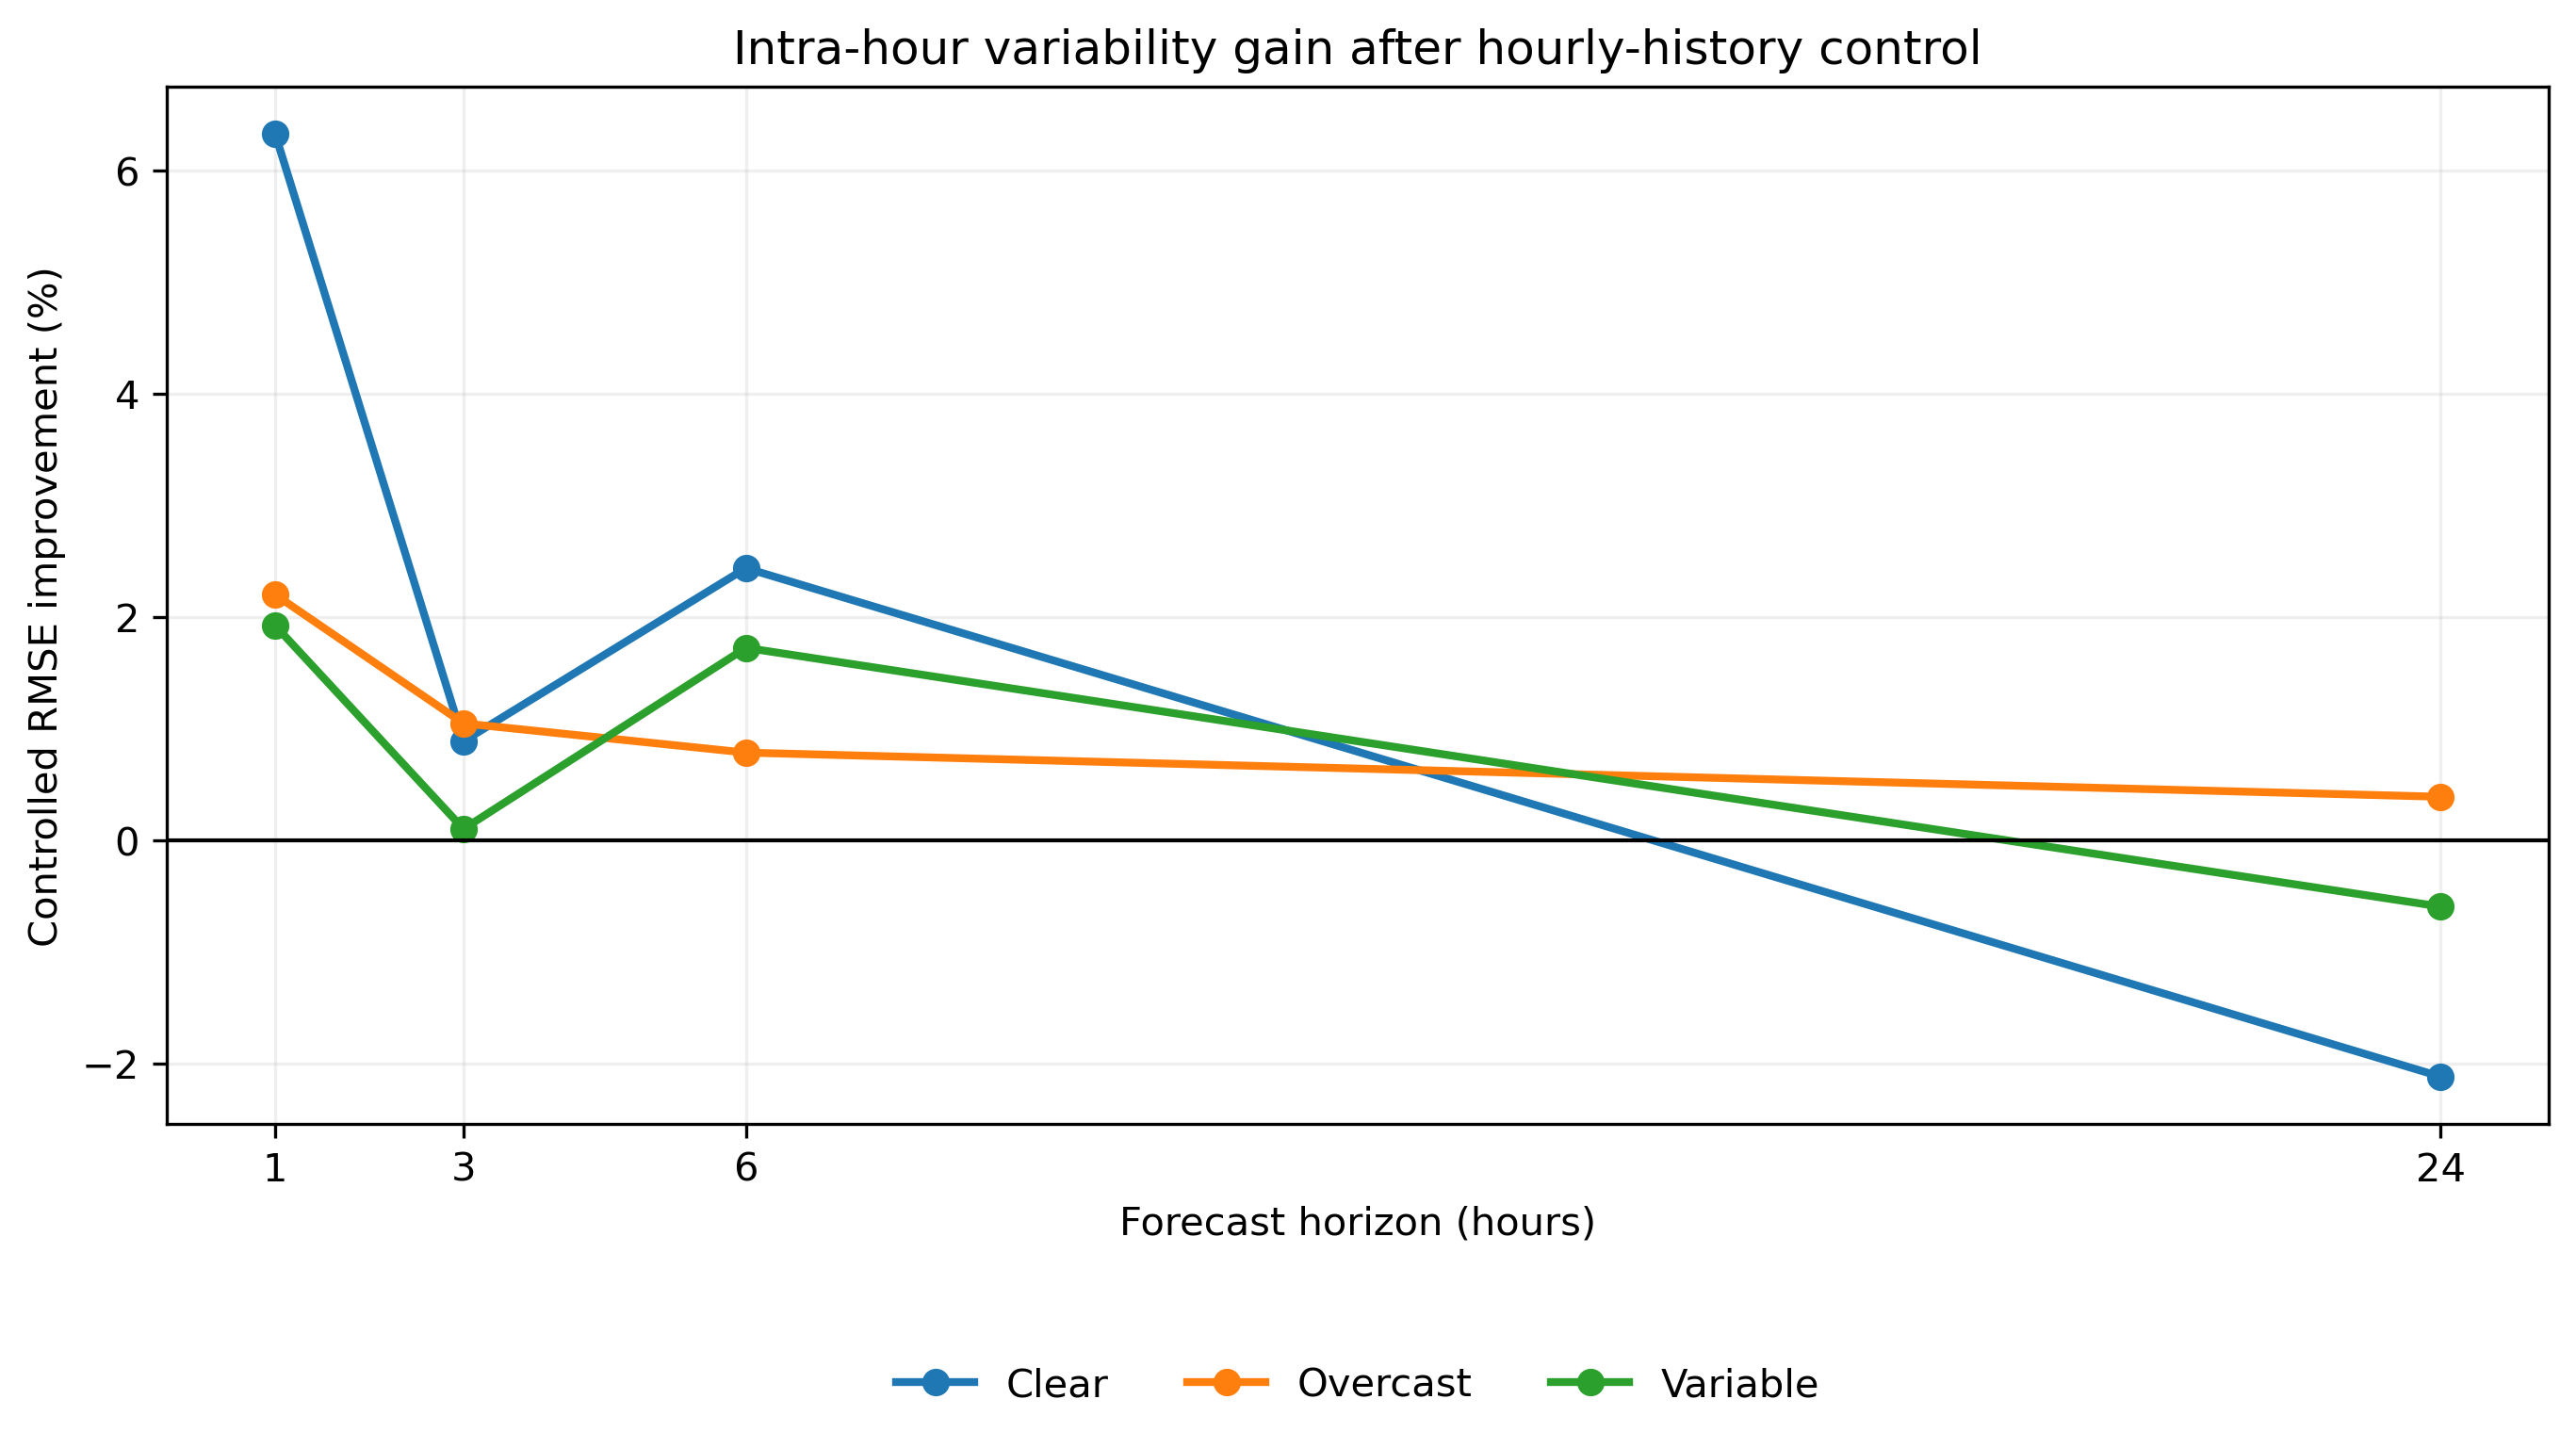
\includegraphics[width=\linewidth,height=0.46\textheight,keepaspectratio]{figures/weather_regime_gain.png}
\caption[Controlled intra-hour gain by daylight weather regime.]{Controlled intra-hour gain by daylight weather regime, from the predeclared history-versus-combined comparison.}\label{fig:ch4_16}\end{figure}

\begin{figure}[!htbp]\centering
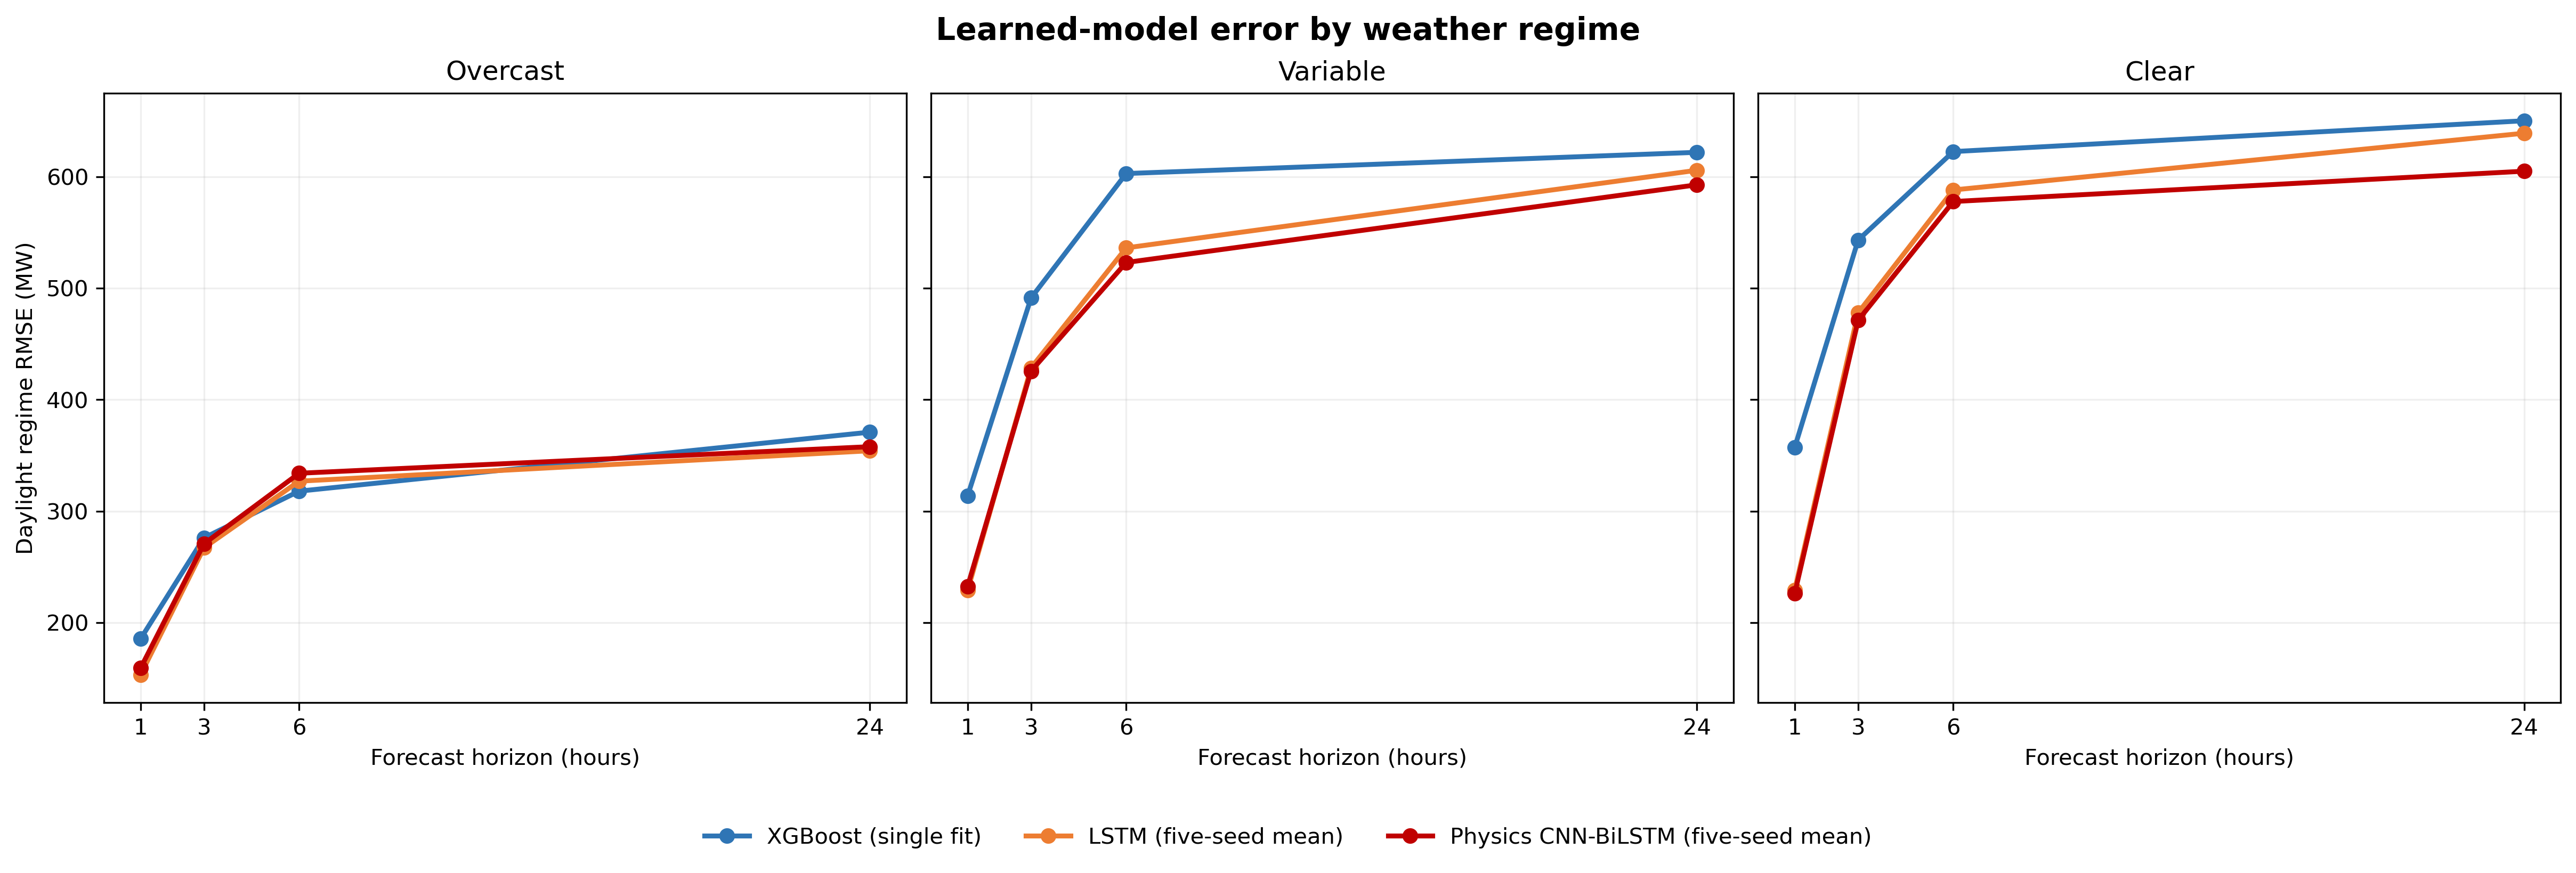
\includegraphics[width=\linewidth,height=0.46\textheight,keepaspectratio]{figures/learned_model_weather_regimes.png}
\caption[Learned-model errors by daylight weather regime.]{Learned-model errors across descriptive daylight weather regimes.}\label{fig:ch4_17}\end{figure}

Individual-seed RMSE confirms training variation. For combined inputs at 24 hours, standard deviation is 2.88 MW for LSTM, 14.91 for CNN-\allowbreak{}BiLSTM and 16.78 for the physics-guided version. Forecast averaging yields the headline values in Table 4.2, which are not the means of seed-level RMSE.

The matched pair has similar 24-hour dispersion, showing that the instability is not created solely by the penalty. Five seeds do not fully characterise training variation, and the paired test intervals do not include it.

The moving-block intervals and Diebold-Mariano tests treat each five-seed mean forecast as fixed. Their uncertainty covers dependence within 2025 and contains no training-variance component, so small neural differences remain conditional on these fitted ensembles.

\begin{figure}[!htbp]\centering
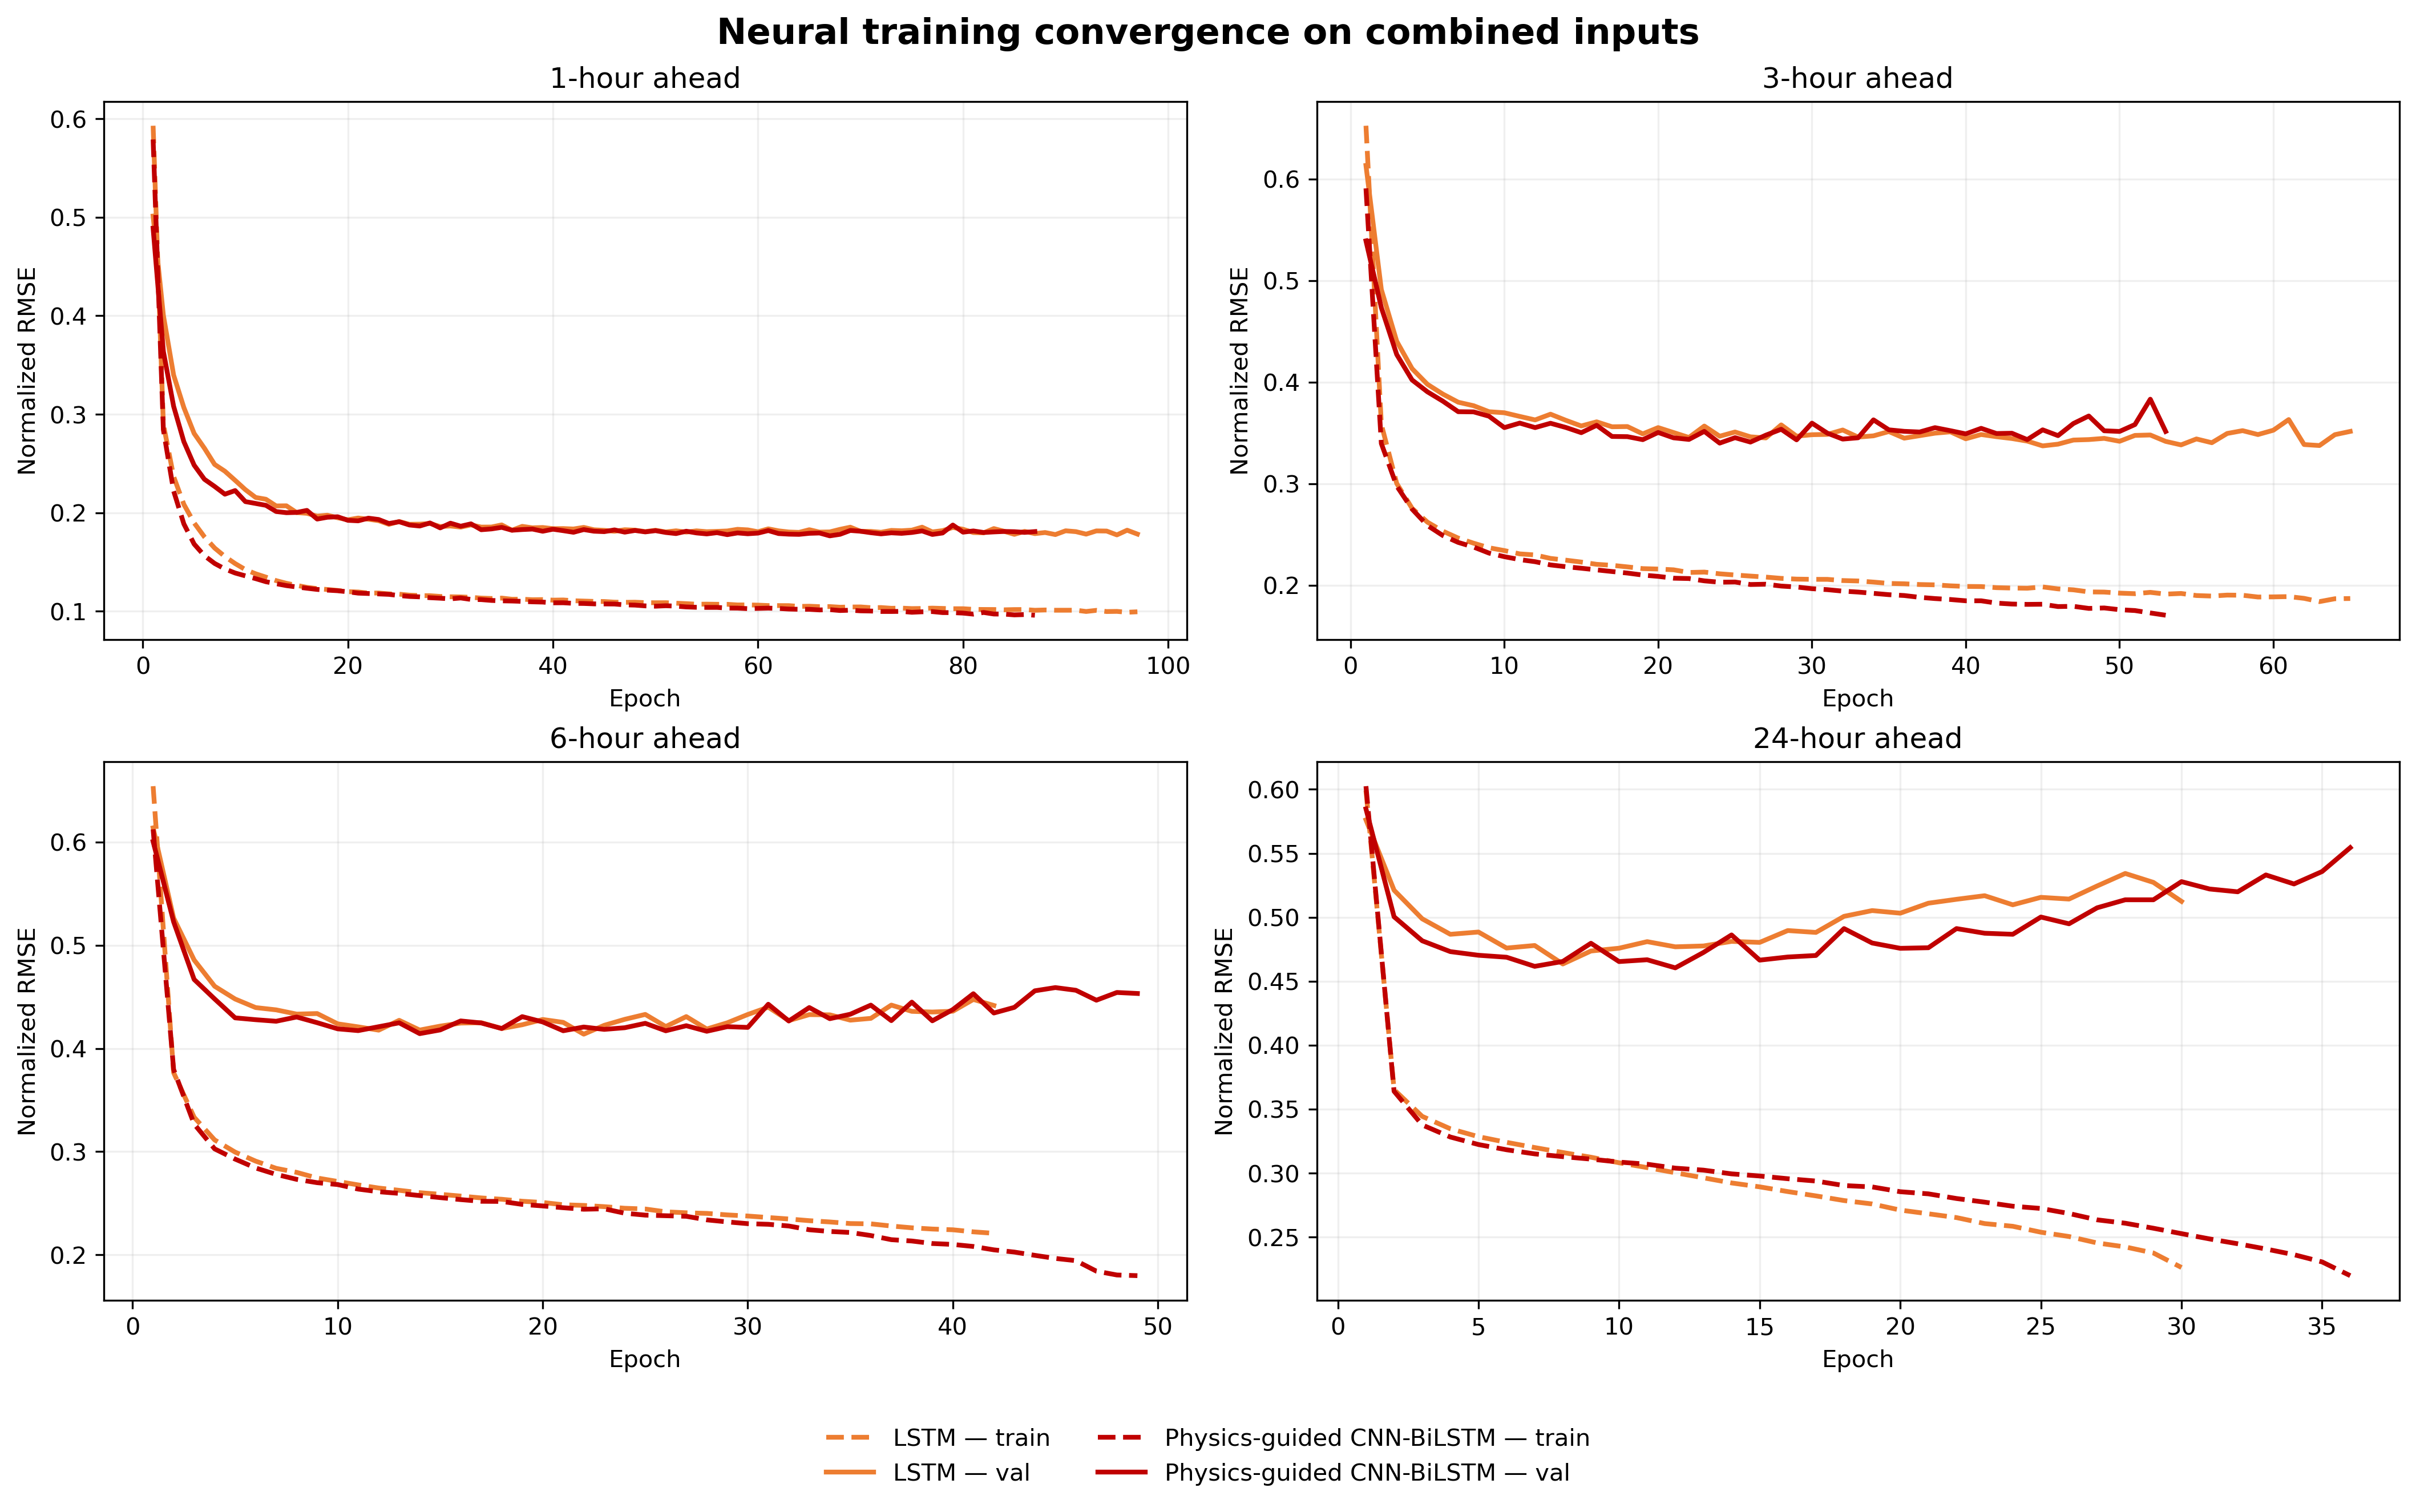
\includegraphics[width=\linewidth,height=0.46\textheight,keepaspectratio]{figures/neural_convergence.png}
\caption[Validation convergence of the neural model fits.]{Validation convergence of the neural model fits.}\label{fig:ch4_18}\end{figure}

The inverse-validation-RMSE ensemble is balanced rather than dominated by one component, yet it never supplies the best combined-input point estimate. Its RMSE is 161.39, 303.88, 373.77 and 407.40 MW, better than XGBoost but worse than the strongest neural model at each horizon.

Weights remain between 0.22 and 0.26, so the result is closer to variance smoothing than specialised regime switching.

The representative trajectories and scatter plots show where aggregate metrics originate. One-hour forecasts follow the daily envelope closely, while longer horizons smooth peaks and underpredict some high-output observations. Dense night-time points near zero improve all-hour scores, whereas daylight scatter widens with horizon. These figures are diagnostic examples, not independent tests.

The evidence hierarchy is consistent. Hourly generation history has the largest effect. Intra-hour summaries add smaller robust gains without history, but after controlling history their support concentrates at 1 hour, with 3 and 6-hour gains for XGBoost and the physics-guided procedure. Physical penalties improve only the 6-hour result robustly. Relative, peak-normalised and absolute RMSE agree, as does the output-scale sensitivity check. Conservative dependence assumptions turn marginal findings inconclusive rather than reversing robust claims, supporting a short-horizon feature conclusion while leaving day-ahead value open. Reporting only the best cell would obscure this pattern: LSTM with combined inputs leads at 1 hour, whereas unconstrained CNN-\allowbreak{}BiLSTM with history but no dispersion leads at 24 hours.

\begin{figure}[!htbp]\centering
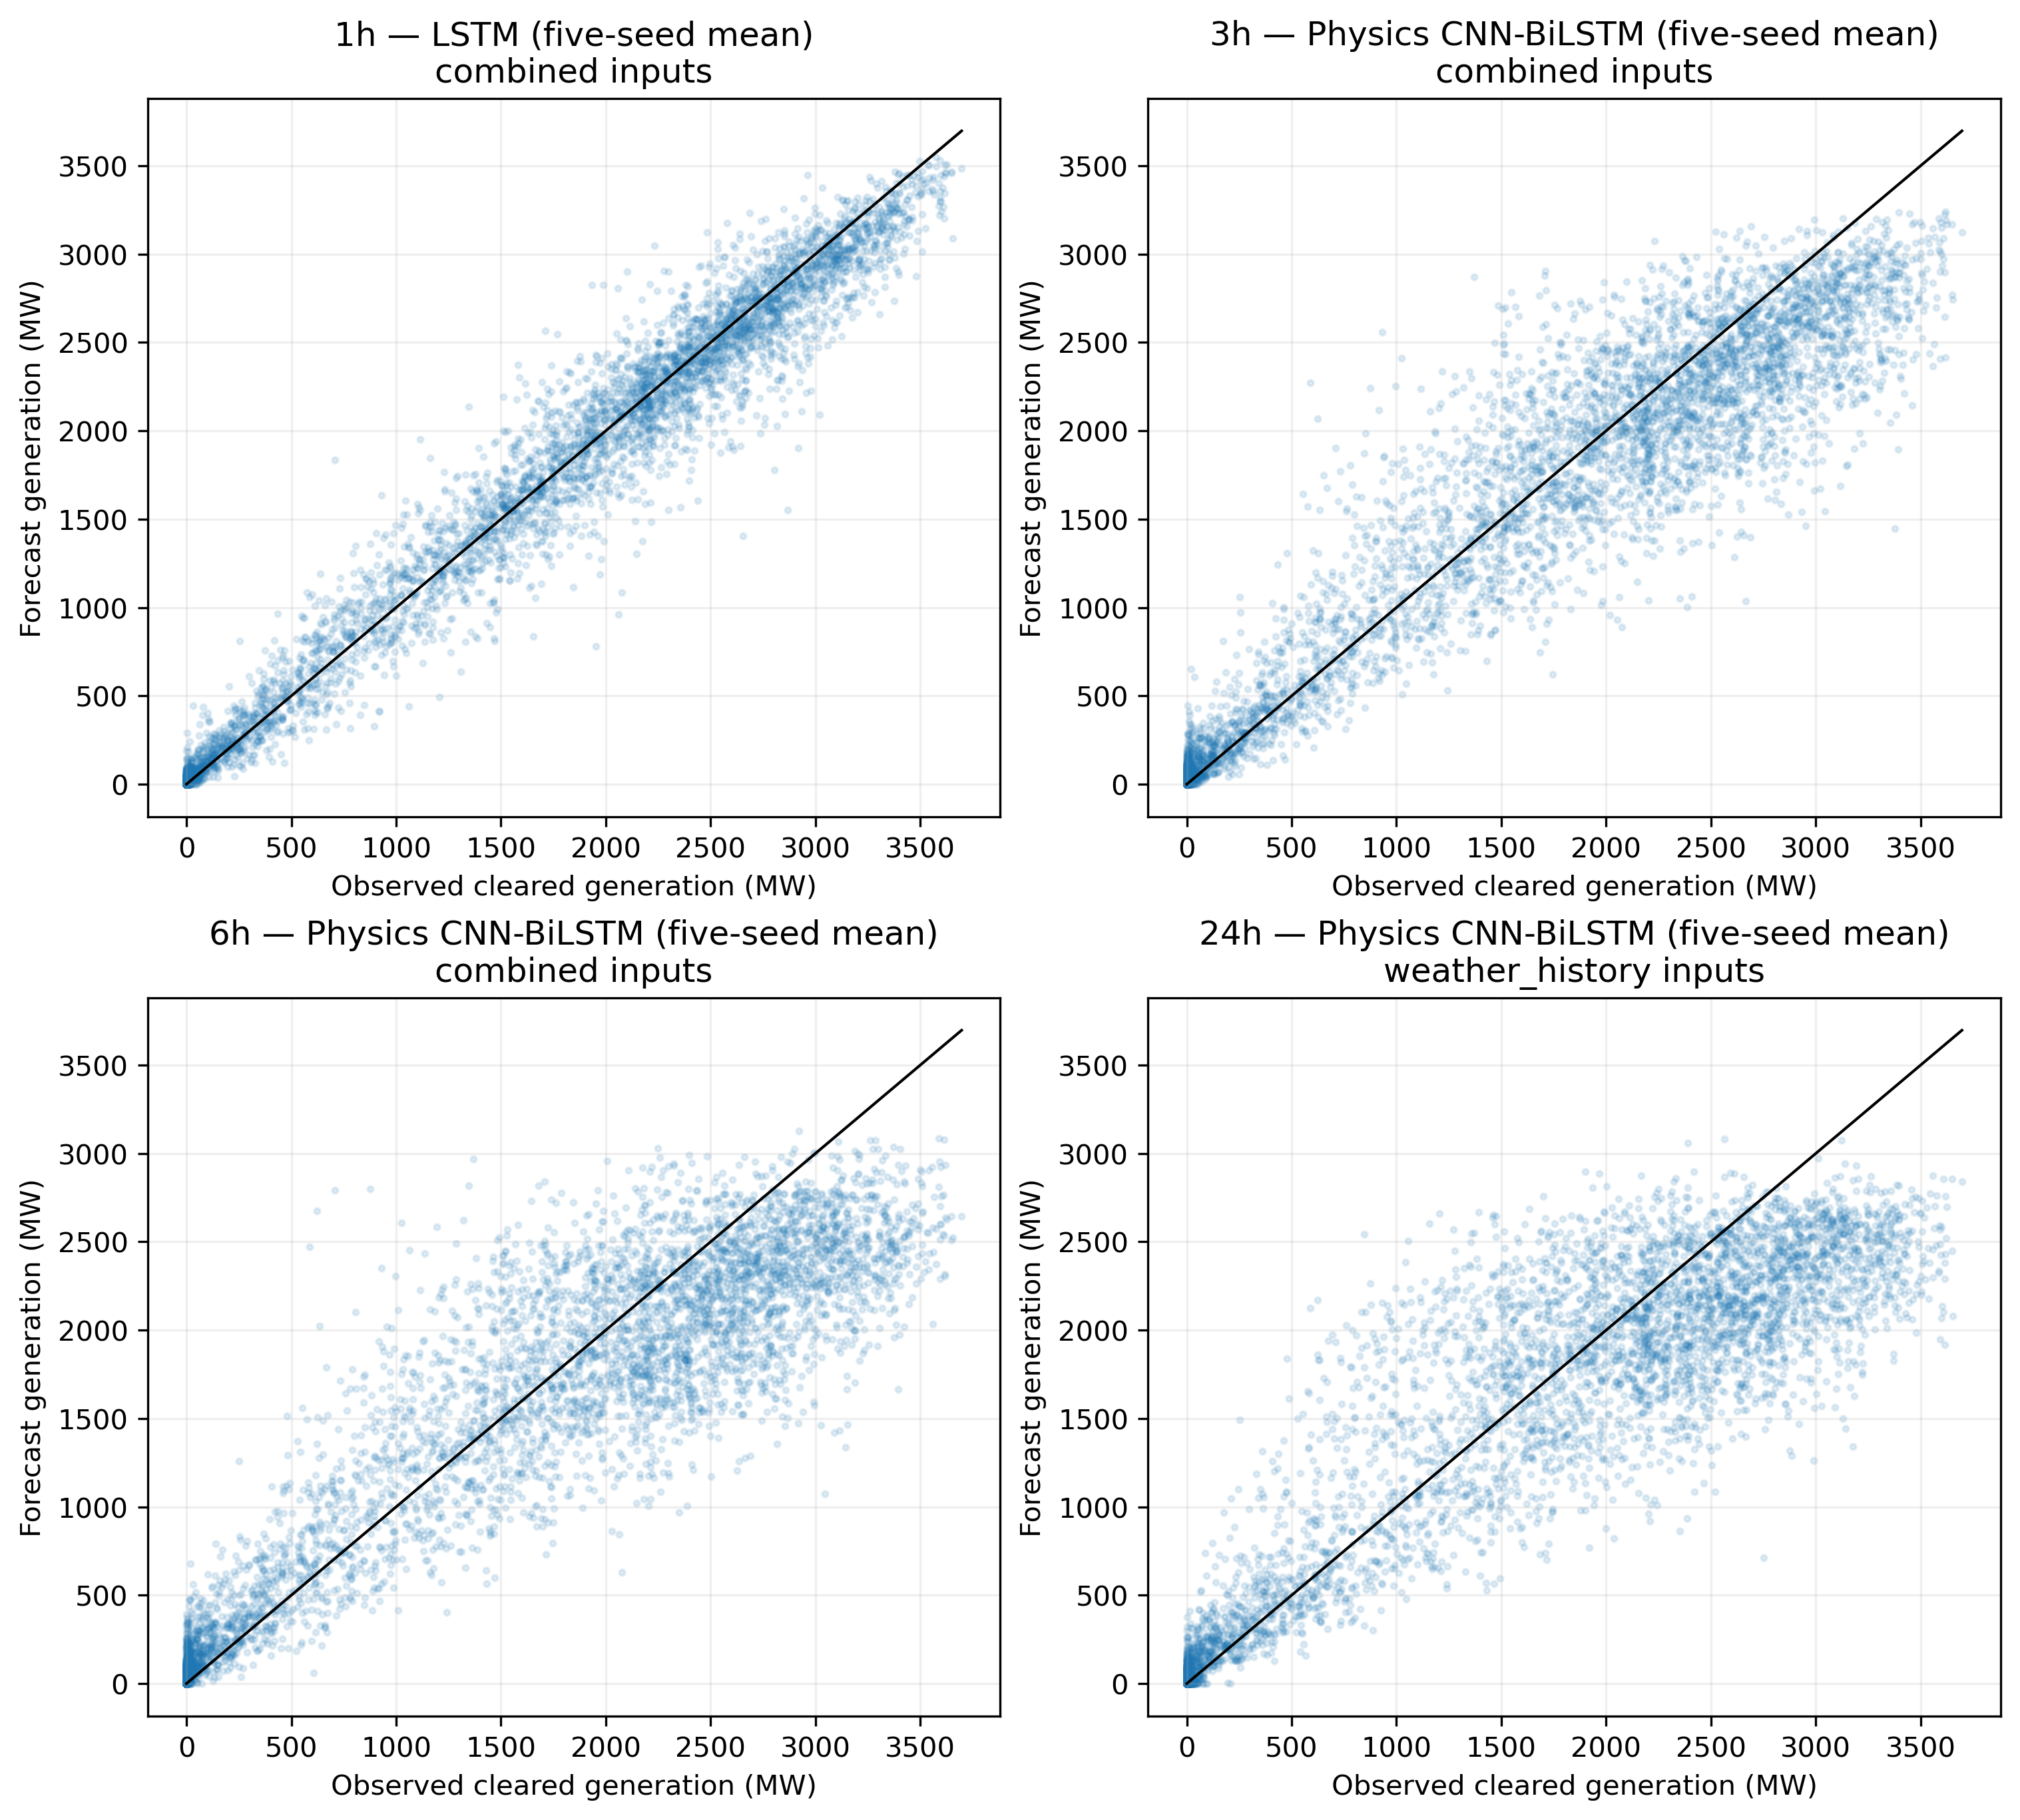
\includegraphics[width=\linewidth,height=0.46\textheight,keepaspectratio]{figures/actual_vs_predicted_test.png}
\caption[Representative observed and predicted test values.]{Representative observed and predicted values on the 2025 test period. Each panel shows the lowest-RMSE learned forecast for that horizon, so the selected model and input set can differ between panels.}\label{fig:ch4_19}\end{figure}

\clearpage

\section{Discussion}

\subsection{Answer to the Research Question}

Scale-normalised five-minute intra-hour features improve short-horizon forecast skill beyond ordinary hourly history, but the result depends on model and horizon. In the controlled comparison, all four learned procedures gain robustly at one hour. XGBoost and the physics-guided CNN-\allowbreak{}BiLSTM also gain robustly at three and six hours, while the LSTM and unpenalised CNN-\allowbreak{}BiLSTM do not satisfy the full decision rule there. No procedure gains robustly at 24 hours. The robust controlled improvements range from 1.63 to 2.86 percent.

The complementary comparison without hourly history is broader but less selective. Adding the two dispersion summaries to meteorology improves all four learned procedures robustly at all four horizons, by 1.26 to 11.46 percent. The meteorological base is weak in absolute terms, including an XGBoost one-hour RMSE of 722.73 MW against persistence at 469.06 MW, because no feature set contains weather for the target period. Part of that gain therefore substitutes for forward weather an operational system would already hold. The controlled comparison is the direct answer because both arms contain the same hourly generation history.

Most of the value of AEMO data therefore comes from the latest hourly level and trailing summaries. Across the learned procedures, they reduce meteorology-only RMSE by 41.03 to 77.07 percent, compared with 1.26 to 11.46 percent for the dispersion columns alone. The five-minute summaries are incremental short-horizon signals, not substitutes for ordinary generation history.

The pattern suggests representation matters: tree splits can use a variability threshold directly, and the physics-guided sequence model benefits at each intraday horizon. The LSTM and unpenalised CNN-\allowbreak{}BiLSTM absorb a robust gain only at one hour under the stringent conjunction rule, possibly because their sequence representations already reconstruct part of the recent dynamics.

The 24-hour reversal is reasonable: variability in the latest completed hour can inform cloud motion over the next few hours but is unlikely to describe conditions a day later, while learned noise or regime-specific associations persist. Chapter 4 offers a second explanation at that horizon, namely that the recurrent fits stop improving after about nine to twelve epochs, so the day-ahead models extract less structure from the same window. This design does not separate the two accounts, so the recommendation to omit the features at 24 hours is precautionary rather than explained. Either way the results favour horizon-specific input policies over assuming that a richer feature vector is universally preferable.

\subsection{The Regime Hypothesis Was Not Supported}

The regime hypothesis predicted the largest intra-hour gain under variable cloud, since coarse hourly reanalysis should miss rapid change. The measured ordering does not support that prediction. Averaged across the four learned procedures, the one-hour gain is 4.13 percent under clear skies, 1.78 percent overcast and 1.13 percent variable. Clear skies also give the largest mean gain at six hours, while the 24-hour means are negative under clear and variable conditions.

This is a failed prediction, not a reversal. The regime breakdown is a secondary subgroup analysis with unequal strata of 578 overcast, 2,008 variable and 1,688 clear hours. It has no multiplicity correction or interval for an individual cell, and the test year had already been inspected. It should not outweigh the result it qualifies.

Two competing accounts fit the observed direction better, and both are testable. The first account is redundancy. Under broken cloud, the hourly mean already contains that hour's cloud-driven variation, so a dispersion summary from the same intervals adds little to the level it accompanies. Under clear skies, the hourly level is nearly predictable from solar geometry and calendar position, so residual dispersion still carries information about departures from that expectation. That account predicts the feature is most useful where hourly history is least informative.

The second is a market-clearing account. Both dispersion features are computed from SS\_\allowbreak{}SOLAR\_\allowbreak{}CLEAREDMW, the same market-cleared series as the target, which sits materially below unconstrained availability at midday. Taking midday as market-clock label hours 10:00 to 14:00 with unconstrained output above 50 MW gives 94,018 intervals. Cleared output is below 99 percent of available output in 75.6 percent of cases, and the mean cleared-to-available ratio is 0.891, falling from 0.909 in 2021 to 0.830 in 2025. Curtailment and dispatch therefore change the coefficient of variation and the relative range directly, so the clear-regime ordering could reflect when clearing departs from available output rather than when dispersion carries weather information. Because the unconstrained series SS\_\allowbreak{}SOLAR\_\allowbreak{}UIGF is present in the same export but excluded, re-deriving the two summaries from it, or stratifying by the cleared-to-available ratio, would separate the explanations. Neither test is reported here, so both accounts remain open.

Two design features limit this account. Eight-site equal-weight averaging smooths the spatial structure that produces real cloud transitions, so the variable regime may be less variable than labelled. The clearness-index thresholds at 0.3 and 0.7 are conventional, so moving them would reassign hours.

The main finding does not depend on the regime result, because the primary comparison was predeclared on the full sample and unaffected by later grouping; what changes is the interpretation, since within-hour dispersion is not most valuable where cloud is most active.

\subsection{Model Interpretation}

The neural models generally outperform XGBoost, though their ordering depends on horizon. LSTM leads at one hour, the physics-guided CNN-\allowbreak{}BiLSTM at three and six hours, and the unpenalised CNN-\allowbreak{}BiLSTM at 24 hours. Both CNN-\allowbreak{}BiLSTM variants robustly outperform XGBoost at every horizon; LSTM does so at 1, 3 and 6 hours. Most neural-to-neural gaps are inconclusive. The exceptions are the CNN-\allowbreak{}BiLSTM variants over LSTM at 24 hours and the physics-guided model over the unpenalised control at six hours.

The matched CNN-\allowbreak{}BiLSTM control isolates the two loss penalties while holding architecture, inputs and training protocol fixed. Their 1.18 percent six-hour gain is robust, but the comparisons at 1, 3 and 24 hours are inconclusive. The evidence therefore supports a horizon-specific penalty effect, not a general advantage or a physical mechanism.

The ensemble adds computation without a point-accuracy advantage on the present objective: balanced validation weights improve on XGBoost but do not beat the strongest neural forecast, and no failure-injection, missing-model or cross-year experiment tests operational resilience.

Model choice should therefore weigh evidence strength against maintenance cost. On combined inputs, the best RMSEs are 155.25 MW for LSTM at one hour, 300.28 and 369.17 MW for the physics-guided model at three and six hours, and 399.77 MW for the unpenalised CNN-\allowbreak{}BiLSTM at 24 hours. The small intraday neural gaps are mostly unresolved, while both CNN-\allowbreak{}BiLSTM variants have clearer day-ahead evidence than LSTM. The best day-ahead input set still excludes the intra-hour variables.

\subsection{Baselines and Horizon Effects}

Persistence is a demanding 24-hour reference because solar output is strongly periodic daily. The physics-guided combined model improves its RMSE by 5.38 percent, but the corrected comparison is not robust at the conservative dependence setting, where weekly serial dependence and family-wise multiplicity apply. At 1-6 hours persistence deteriorates as the target crosses the solar ramp, so SARIMA is the more informative short-horizon comparator: all three neural procedures robustly outperform it at every horizon, while XGBoost does not at one hour.

Skill is therefore reference-dependent. A 77.38 percent improvement over six-hour persistence sounds dramatic, but persistence is unsuitable across a solar-cycle transition and the forecast improves less against SARIMA. A small day-ahead persistence gain only means that copying the latest hour to the same clock time a day later captures much of the daily pattern.

\subsection{Relation to Previous Research}

The result is consistent with work emphasising complementary data sources and recent generation history \cite{rabault2025datafusion}, while narrowing the claim through a controlled ablation. Prior work on intra-hour irradiance variability motivates the feature design \cite{huang2016intra}, but this project forecasts regional market-cleared generation rather than site irradiance, so its effect sizes and mechanism should not transfer.

Two published effect sizes frame the magnitudes: Perera et al. \cite{perera2022multires} report a 3.81 percent average MASE reduction from forecast combinations, and Abdullah and Mohammed \cite{abdullah2026physics} report GHI RMSE of 19.53 W/m2 against 30.64 W/m2 for attention-based alternatives. The robust controlled gains of 1.63 to 2.86 percent are of the same order as the first and smaller than the second, but targets, inputs and protocols differ, so the comparison is contextual, not a replication.

MERRA-2 supports a reproducible historical benchmark \cite{pfenninger2016longterm}, but it is retrospective reanalysis, not an operational forecast available at issue time, so the study evaluates conditional skill with historical weather fields and does not quantify performance under live numerical weather prediction latency or error. The physics-guided literature \cite{abdullah2026physics} supports domain constraints, but the present loss is narrower than an irradiance-to-power physical model, and sequence-to-sequence methods \cite{mukhoty2019seq2seq} are not reproduced, since each horizon uses an independent scalar-output model.

The benchmark also differs from plant-level PV studies in scale. Regional averaging reduces plant noise, while NSW-wide clouds, capacity additions and dispatch constraints add non-stationarity. Market-cleared generation is not interchangeable with irradiance or AC power, so agreement with earlier rankings is convergence, not replication.

\subsection{Strengths and Limitations}

The main strengths are a chronological held-out year, exact elapsed-time alignment, prevention of gap-bridging sequences, conservative duplicate handling, common windows, five neural seeds, feature-neutral XGBoost tuning, a complete four-model factorial and dependence-sensitive inference. The matched CNN-\allowbreak{}BiLSTM control separates the loss penalties from the architecture.

Several limitations bound the conclusions. First, 2025 is one test year: moving-block intervals describe uncertainty within that year, not variation across future years or fleet growth, and contain no training-seed component. Second, the target excludes most rooftop PV, which nationally supplied 13.9 percent of electricity generation in 2025 against 7.7 percent for utility-scale solar \cite{cec2026clean}, so the segment outside this benchmark is the larger one; the target also includes market interventions and curtailment. Third, eight-site mean reanalysis cannot resolve all spatial cloud motion. The locations are population centres spanning the coast and inland slopes, chosen as a coast-to-inland spread of regional weather proxies with no capacity weighting and no formal site-selection procedure. Inland generation may therefore be under-represented. Fourth, operational feature availability, ingestion delay and live forecast quality are untested. Fifth, XGBoost uses one fitted model per block while neural forecasts average five fits, so between-procedure point estimates do not share the same seed averaging. Sixth, clipping at zero affects a non-trivial share of outputs, and the regime and feature-importance analyses are descriptive rather than causal. Finally, the tested five-minute representation contains only two summaries of the latest completed hour, not ramp timing, interval order or the raw twelve values.

Inference remains conditional on several choices: moving blocks approximate serial dependence but cannot reproduce every seasonal or regime transition, and Bonferroni correction is conservative and reduces power. The intersection rule is more demanding, because one unstable diagnostic changes the label to inconclusive, which explains cases such as the LSTM six-hour gain.

The input control is stronger than a broad ablation but is not a randomised causal intervention. Adding two columns can change optimisation paths, tree splits and learned regularisation. The reported gain therefore belongs to the complete training procedure with or without those columns, not to the energy value of variability.

The duplicate policy is the least assumptive choice for the legacy archive: keeping the first or last row would make the target depend on file ordering, and averaging conflicting rows could create a value matching neither dispatch scenario. Dropping a conflicting group loses data but keeps the target interpretable; no excluded hour occurs in the test year, so the direct test metrics are unaffected, though the training sample can still shift through the 120 excluded hourly bins.

\subsection{Implications}

For this NSW1 task, recent hourly generation should be a core operational input. The two intra-hour summaries are candidates at short horizons, where robust controlled gains range from 1.63 to 2.86 percent. They are robust for XGBoost and the physics-guided model at 1, 3 and 6 hours, and for the LSTM and unpenalised CNN-\allowbreak{}BiLSTM at one hour only. Their value is conditional on reliable five-minute telemetry, and no cost side is estimated here, so the ingestion decision remains open. At one hour XGBoost remains much weaker at 230.70 MW than LSTM at 155.25 MW despite its feature gain. At 24 hours the features should not be assumed beneficial.

No architecture dominates every horizon. LSTM is strongest at one hour, the physics-guided model at three and six hours, and the unpenalised CNN-\allowbreak{}BiLSTM at 24 hours. Deployment would still require issue-time weather, latency monitoring, missing-data fallback, capacity-growth recalibration and out-of-year validation, and RMSE cannot be converted to trading value without prices, exposure and a decision model.

A staged deployment study would begin with shadow forecasts timestamping each prediction and recording every feature's publication time, then monitor performance by horizon, daylight condition, output level and missing-data state.

Capacity growth and interpretability stability also deserve work, and computational reproducibility should not be confused with numerical identity.

\clearpage

\section{Conclusion}

\subsection{Summary}

This study asked to what extent AEMO five-minute intra-hour features improve short-term solar PV forecast skill over meteorological inputs alone in New South Wales. The controlled answer is positive at short horizons and disappears at 24 hours. All four learned procedures gain robustly at one hour; XGBoost and the physics-guided CNN-\allowbreak{}BiLSTM also gain at three and six hours, while the LSTM and unpenalised CNN-\allowbreak{}BiLSTM do not satisfy the full decision rule there. No procedure gains robustly at 24 hours.

Robust controlled gains range from 1.63 to 2.86 percent, while ordinary hourly history supplies the dominant reduction. In the complementary comparison without history, all four procedures improve robustly at every horizon by 1.26 to 11.46 percent. Throughout this report, robust means agreement across interval, Diebold-Mariano and output-scale checks within the 2025 test year, and the intervals contain no training-seed component.

On combined inputs, LSTM records the lowest one-hour RMSE at 155.25 MW, the physics-guided model leads at three and six hours with 300.28 and 369.17 MW, and the unpenalised CNN-\allowbreak{}BiLSTM leads at 24 hours with 399.77 MW. Its weather\_\allowbreak{}history result of 390.54 MW is the lowest day-ahead feature-set value, showing that the intra-hour addition is not automatically helpful. The matched CNN-\allowbreak{}BiLSTM comparison attributes a robust 1.18 percent gain to the loss penalties only at six hours. The ensemble improves on XGBoost but not on the best neural forecast. These findings concern 2025 market-cleared utility-scale generation under retrospective reanalysis, not rooftop PV, unconstrained production or economic value.

\subsection{Contributions}

The primary contribution is an answer to the research question: AEMO five-minute intra-hour features carry a modest short-horizon increment beyond ordinary hourly history, with no robust day-ahead benefit. The evidence base is a self-contained regional benchmark joining AEMO five-minute generation with hourly weather, a duplicate and alignment policy, and a four-set feature design. Four learned procedures and three baselines are evaluated on common windows, with five averaged seeds for each neural procedure. A controlled result counts as robust only when block-bootstrap intervals, multiple Diebold-Mariano bandwidths and an alternative output scale agree. The notebook completed from a fresh kernel on Apple Silicon using MPS.

The evaluation controls also transfer: exact elapsed-time joins stop missing observations from silently redefining a horizon, contiguous sequences stop a recurrent model from treating gaps as adjacent hours, and multiple dependence bandwidths reveal when a significant result relies on a short-memory assumption.

Two findings extend beyond that answer. First, the complete factorial design separates the frequency of a data source from its incremental information across all four procedures. Without hourly history, gains range from 1.26 to 11.46 percent and are robust in all 16 cells. After controlling for history, the robust gains narrow to 1.63 to 2.86 percent and occur in eight of 16 cells. The increment shrinks as a completed hour's mean becomes available, which argues for controlled ablations over single-baseline comparisons.

Second, validation error bottomed out after roughly sixty epochs at one hour but within about nine to twelve epochs at day-ahead range. The recurrent models therefore extracted far less structure from an identical input window as the horizon lengthened, reframing a model-ranking result as a training-behaviour result.

\subsection{Recommendations and Future Work}

An operational extension should replace reanalysis with archived issue-time weather forecasts, reproduce the comparison across held-out years and other NEM regions, and define latency, record conflicts, missing-feature fallbacks, capacity-change monitoring and retraining triggers.

Further experiments should vary the penalty weights and constraints within the matched CNN-\allowbreak{}BiLSTM design, and test whether richer intra-hour representations add value beyond the two summaries. Probabilistic forecasts should be assessed with calibration, coverage and sharpness rather than point RMSE alone, and regime and ramp-event evaluation predeclared and powered. When additional years become available, rolling-origin evaluation would show whether the controlled feature effect persists through different weather years and fleet growth, while cross-region evaluation could separate NSW-specific conclusions from general properties of utility-scale solar forecasting.

Operational research should preserve the same data rules: auditable quarantine for conflicting records, deterministic de-duplication of identical re-deliveries, a documented fallback rather than silent zero filling, and publication timestamps instead of assumed immediate availability. Forecast value should also be measured in the decision context, since an operator may prioritise ramp warnings while a participant faces imbalance costs.

The recommended sequence is evidence-led: preserve hourly generation history and the strong baselines, add the two scale-normalised intra-hour summaries where each deployed model has a robust controlled gain, and omit them at 24 hours. Architecture should be chosen under measured latency and maintenance constraints rather than treating small RMSE gaps as decisive. Only then should a richer ensemble or high-frequency representation follow. The next validation should predeclare what would change this conclusion: retain the intra-hour columns only where the controlled gain remains positive with a 168-hour interval excluding zero and the corrected Diebold-Mariano and output-scale checks agree. Latency should be tested on archived issue-time weather or audited AEMO publication timestamps, and regime and ramp-event tests should state their required sample size before the strata are inspected.

This sequence protects the main conclusion from deployment-architecture changes: even if a future transformer, probabilistic model or improved weather source lowers absolute error, the controlled question can be repeated: does five-minute variability add information beyond the latest hourly level and trailing history?

\subsection{Closing Statement}

Recent hourly generation is the central predictive input in this benchmark. Five-minute variability adds smaller but repeatable short-horizon information over meteorological inputs alone, and its day-ahead value is unsupported, favouring controlled feature integration over claims that higher-frequency data or greater model complexity must improve every horizon. The tested object is two scale-normalised scalars computed from the twelve five-minute values of the latest completed hour; ramp timing, within-hour shape and the raw twelve values were not tested, so the finding concerns this representation, not five-minute sampling in general.

\clearpage

\phantomsection
\addcontentsline{toc}{section}{References}
% The reference list is written out in references.tex, so the printed number
% always equals the in-text number. Do not replace this with \bibliography{bib}:
% a BibTeX run renumbers the printed list into citation order.
\begin{thebibliography}{37}
\bibitem[1]{perera2024dayahead} M.~Perera, J.~D. Hoog, K.~Bandara, D.~Senanayake, and S.~Halgamuge, ``Day-ahead
  regional solar power forecasting with hierarchical temporal convolutional
  neural networks using historical power generation and weather data,'' 2024.
\newblock arXiv:2403.01653.
\bibitem[2]{schubnel2025solarcross} B.~Schubnel, J.~Simeunovi\'c, C.~Tissier, P.-J. Alet, and R.~E. Carrillo,
  ``Solarcrossformer: Improving day-ahead solar irradiance forecasting by
  integrating satellite imagery and ground sensors,'' 2025.
\newblock arXiv:2509.15827.
\bibitem[3]{scott2025transformers} A.~Scott, S.~Sreedhara, and F.~Ayoola, ``Transformers applied to short-term
  solar pv power output forecasting,'' 2025.
\newblock arXiv:2505.03188.
\bibitem[4]{huang2016intra} J.~Huang and R.~J. Davy, ``Predicting intra-hour variability of solar
  irradiance using hourly local weather forecasts,'' {\em Sol. Energy},
  vol.~139, pp.~633--639, 2016.
\bibitem[5]{prasad2021prediction} A.~A. Prasad and M.~Kay, ``Prediction of solar power using near-real time
  satellite data,'' {\em Energies}, vol.~14, p.~5865, 2021.
\bibitem[6]{bom2022ecl} B.~of~Meteorology, ``About east coast lows.'' Australian Government, 2022.
\bibitem[7]{pfenninger2016longterm} S.~Pfenninger and I.~Staffell, ``Long-term patterns of european pv output using
  30 years of validated hourly reanalysis and satellite data,'' {\em Energy},
  vol.~114, pp.~1251--1265, 2016.
\bibitem[8]{renewables2025api} Renewables.ninja, ``Api documentation,'' 2025.
\bibitem[9]{aemo2024nemosis} A.~E.~M. Operator, ``Mmsdm historical data: Dispatchregionsum,'' 2024.
\newblock Accessed via the NEMOSIS dynamic data compiler.
\bibitem[10]{ramirez2020simulation} L.~R. Camargo and J.~Schmidt, ``Simulation of long-term time series of solar photovoltaic power: Is the ERA5-land reanalysis the next big step?'' {\em Sustain. Energy Technol. Assess.}, p.~100829, 2020.
\bibitem[11]{nielsen2021irradiancenet} A.~H. Nielsen, A.~Iosifidis, and H.~Karstoft, ``Irradiancenet: Spatiotemporal
  deep learning model for satellite-derived solar irradiance short-term
  forecasting,'' {\em Sol. Energy}, vol.~228, pp.~659--669, 2021.
\bibitem[12]{voyant2025clearsky} C.~Voyant, M.~Despotovic, G.~Notton, Y.-M. Saint-Drenan, M.~Asloune, and
  L.~Garcia-Gutierrez, ``On the importance of clearsky model in short-term
  solar radiation forecasting,'' {\em Sol. Energy}, vol.~289, p.~113490, 2025.
\bibitem[13]{mukhoty2019seq2seq} B.~P. Mukhoty, V.~Maurya, and S.~K. Shukla, ``Sequence to sequence deep
  learning models for solar irradiation forecasting,'' 2019.
\newblock arXiv:1904.13081.
\bibitem[14]{rabault2025datafusion} J.~Rabault, M.~L. Saetra, A.~Dobler, S.~Eastwood, and E.~Berge, ``Data fusion
  of complementary data sources using machine learning enables higher accuracy
  solar resource maps,'' 2025.
\newblock arXiv:2501.04381.
\bibitem[15]{wen2026multisource} X.~Wen, Y.~Zhang, X.~Liu, G.~Wang, and Y.~Zhang, ``Multi-source fusion-based
  cross-dimensional temporal feature-enhanced photovoltaic forecasting model,''
  {\em Renewable Energy}, vol.~266, p.~125658, 2026.
\bibitem[16]{mollasalehi2025review} A.~Mollasalehi and A.~Farhadi, ``Solar and wind power forecasting: a
  comparative review of lstm, random forest, and xgboost models,'' 2025.
\newblock arXiv:2509.24059.
\bibitem[17]{feng2018clustering} C.~Feng, M.~Cui, B.-M. Hodge, S.~Lu, and H.~F. Hamann, ``An unsupervised
  clustering-based short-term solar forecasting methodology using multi-model
  machine learning blending,'' 2018.
\newblock arXiv:1805.04193.
\bibitem[18]{perera2022multires} M.~Perera, J.~D. Hoog, K.~Bandara, and S.~Halgamuge, ``Multi-resolution,
  multi-horizon distributed solar pv power forecasting with forecast
  combinations,'' {\em Expert Syst. Appl.}, vol.~205, p.~117690, 2022.
\bibitem[19]{sudharshan2026spatiotemporal} K.~Sudharshan, C.~Naveen, and R.~C. Bansal, ``Spatiotemporal solar irradiance
  forecasting and seasonal pattern recognition for intelligent pv integration
  using deep learning,'' {\em Sol. Energy}, vol.~316, p.~114895, 2026.
\bibitem[20]{abdullah2026physics} M.~E.~B. Abdullah and R.~A.~I. Mohammed, ``Outperforming self-attention
  mechanisms in solar irradiance forecasting via physics-guided neural
  networks,'' 2026.
\newblock arXiv:2604.13455.
\bibitem[21]{hoang2025efficient} T.~Hoang, ``Efficient deep learning for short-term solar irradiance time series
  forecasting: a benchmark study in ho chi minh city,'' 2025.
\newblock arXiv:2512.23898.
\bibitem[22]{basu2026solartransformer} A.~Basu, J.~Roy, A.~Datta, P.~Sanyal, and S.~Banerjee, ``Solartformer: A
  transformer based deep learning approach for short term solar power
  forecasting,'' 2026.
\newblock arXiv:2604.24306.
\bibitem[23]{lu2025ctpatchtst} K.~Lu, M.~Huo, Y.~Li, Q.~Zhu, and Z.~Chen, ``Ct-patchtst: Channel-time patch
  time-series transformer for long-term renewable energy forecasting,'' 2025.
\newblock arXiv:2501.08620.
\bibitem[24]{dao2020ensemble} L.~A. Dao, L.~Ferrarini, and D.~L. Carrubba, ``Improving solar and pv power
  prediction with ensemble methods,'' 2020.
\newblock arXiv:2011.09950.
\bibitem[25]{voyant2025nice} C.~Voyant, M.~Despotovic, L.~Garcia-Gutierrez, R.~A. e~Silva, P.~Lauret,
  T.~Soubdhan, and N.~Bailek, ``Nice$^k$ metrics: Unified and multidimensional
  framework for evaluating deterministic solar forecasting accuracy,'' {\em
  Sustain. Energy Technol. Assess.}, p.~104588, 2025.
\bibitem[26]{pedro2012assessment} H.~T.~C. Pedro and C.~F.~M. Coimbra, ``Assessment of forecasting techniques for
  solar power production with no exogenous inputs,'' {\em Solar Energy},
  vol.~86, no.~7, pp.~2017--2028, 2012.
\bibitem[27]{diebold1995comparing} F.~X. Diebold and R.~S. Mariano, ``Comparing predictive accuracy,'' {\em
  Journal of Business and Economic Statistics}, vol.~13, no.~3, pp.~253--263,
  1995.
\bibitem[28]{boland2022forecasting} J.~Boland, S.~Farah, and L.~Bai, ``Forecasting of wind and solar farm output in the Australian National Electricity Market: A review,'' {\em Energies}, vol.~15, no.~1, p.~370, 2022.
\bibitem[29]{farah2021time} S.~Farah and J.~Boland, ``Time series model for real-time forecasting of Australian photovoltaic solar farms power output,'' {\em J. Renew. Sustain. Energy}, vol.~13, no.~4, p.~046102, 2021.
\bibitem[30]{lorenz2009irradiance} E.~Lorenz, J.~Hurka, D.~Heinemann, and H.~G. Beyer, ``Irradiance forecasting for the power prediction of grid-connected photovoltaic systems,'' {\em IEEE J. Sel. Topics Appl. Earth Observ. Remote Sens.}, vol.~2, no.~1, pp.~2--10, 2009.
\bibitem[31]{huang2018assessing} J.~Huang, L.~J. Rikus, Y.~Qin, and J.~Katzfey, ``Assessing model performance of daily solar irradiance forecasts over Australia,'' {\em Sol. Energy}, vol.~176, pp.~615--626, 2018.
\bibitem[32]{yang2020verification} D.~Yang et al., ``Verification of deterministic solar forecasts,'' {\em Sol. Energy}, vol.~210, pp.~20--37, 2020.
\bibitem[33]{yang2019guideline} D.~Yang, ``A guideline to solar forecasting research practice: Reproducible, operational, probabilistic or physically-based, ensemble, and skill (ROPES),'' {\em J. Renew. Sustain. Energy}, vol.~11, no.~2, p.~022701, 2019.
\bibitem[34]{yang2022historical} D.~Yang, W.~Wang, and T.~Hong, ``A historical weather forecast dataset from the European Centre for Medium-Range Weather Forecasts (ECMWF) for energy forecasting,'' {\em Sol. Energy}, vol.~232, pp.~263--274, 2022.
\bibitem[35]{aemo2026datamodel} A.~E.~M. Operator, ``Electricity data model report,'' AEMO Electricity Data Model v5.7.0, Report 57, 2026. Defines SS\_SOLAR\_UIGF and SS\_SOLAR\_CLEAREDMW.
\bibitem[36]{aemo2022handbook} A.~E.~M. Operator, ``NEM operational forecasting and dispatch handbook for wind and solar generators,'' Australian Energy Market Operator, Version 1.3, Sep. 2022.
\bibitem[37]{cec2026clean} C.~E. Council, ``Clean energy Australia report 2026,'' Clean Energy Council, Melbourne, Australia, 2026.
\end{thebibliography}


\clearpage

\addcontentsline{toc}{section}{Appendix}
\subsection*{Appendix A: Data Sources and Licences}

The generation source is AEMO DISPATCHREGIONSUM for NSW1, retrieved through NEMOSIS. The legacy export lacks intervention labels. Exact-value duplicate timestamps are collapsed; conflicting timestamp groups are dropped because the normal-dispatch observation cannot be identified. Hourly meteorology comes from renewables.ninja for Sydney, Newcastle, Wollongong, Central Coast, Tamworth, Bathurst, Orange and Dubbo. Source attribution and access conditions should accompany redistribution of archived data. The simulated renewables.ninja PV series is excluded from prediction inputs.

\subsection*{Appendix B: Reproducibility Configuration}

\setcounter{table}{0}
\renewcommand{\thetable}{B.\arabic{table}}

Table~\ref{tab:app_b1} records the final training and evaluation configuration.

\begin{table}[h!]
\centering
\caption{Reproducibility configuration summary.}
\label{tab:app_b1}
\footnotesize
\begin{tabularx}{\linewidth}{|l|X|}
\hline
\textbf{Component} & \textbf{Setting} \\
\hline
Chronological split & train September 2020 to 2023; validation 2024; test 2025 \\
Feature sets & weather (11), weather\_intra (13), weather\_history (14), combined (16) \\
Forecast horizons & 1, 3, 6 and 24 hours; direct scalar model per horizon \\
Sequence construction & contiguous 24-hour windows; exact elapsed-time target matching \\
LSTM & one layer; 64 hidden units \\
CNN-BiLSTM control & Conv1D 32 filters, kernel 3; max pool; bidirectional LSTM 64; head 128 \\
Physics-guided model & architecture matched to CNN-BiLSTM control \\
Physics-guided loss & MSE plus 0.1 times negative-output and night-time zero penalties \\
Optimisation & batch 512; learning rate 0.001; maximum 100 epochs \\
Early stopping & patience 20; best validation checkpoint restored \\
Random seeds & 42, 123, 456, 789 and 1024 \\
XGBoost & 30 Optuna trials per feature set and horizon; horizon setting selected by mean validation RMSE across all four sets \\
Ensemble & inverse validation-RMSE weights across four learned models \\
Significance testing & Diebold-Mariano bandwidths h-1, 24 and 168; family-wise Bonferroni \\
Bootstrap CIs & 95\%; 2,000 moving-block resamples; 24, 48 and 168-hour blocks \\
Final hardware & Apple Silicon arm64; PyTorch MPS \\
Final environment & conda spunky; Python 3.12.12; PyTorch 2.5.1; XGBoost 3.0.1 \\
Execution & 14 September 2026; clean kernel; 30 code cells; no errors or stderr \\
Notebook SHA-256 & 334693053e09254bdb10d1b4a5f628df\allowbreak{}0e1c2b9b06ac2e744adea0d84c00b4f6 \\
Digest command & sha256sum applied to the notebook file itself; the value is reproduced in the run manifest and checked by the verification script on every build \\
\hline
\end{tabularx}
\end{table}

\subsection*{Appendix C: Literature Search Protocol and Screening Flow}

The retained set was assembled in July 2026 from two databases. arXiv was queried through 15 Boolean expressions combining terms such as solar PV forecasting, machine learning, irradiance, LSTM, physics-guided and reanalysis. Semantic Scholar was queried through three broader expressions. Coverage was 2020 to 2026, with foundational pre-2020 papers retained where they established architectures still in use. Inclusion required machine learning or statistical forecasting of solar irradiance or PV generation with reported quantitative error metrics. Exclusion covered wind-only forecasting, papers without reported metrics, and hardware or policy analysis. Screening was conducted by a single reviewer.

\setcounter{table}{0}
\renewcommand{\thetable}{C.\arabic{table}}

Table~\ref{tab:app_c1} records the screening flow as the notes report it.

\begin{table}[h!]
\centering
\caption{Literature screening flow, July 2026.}
\label{tab:app_c1}
\footnotesize
\begin{tabularx}{\linewidth}{|l|X|}
\hline
\textbf{Stage} & \textbf{Count or decision} \\
\hline
arXiv Boolean queries run & 15 \\
Semantic Scholar queries run & 3 \\
arXiv records returned & approximately 1,300,000 \\
Retained at title and abstract screening & 18 \\
Added from Semantic Scholar & 3 \\
Added from citation tracking & 2 \\
Added from targeted Crossref search & 3 \\
Retained items in total & 26 \\
Designated key references in the notes & 12 \\
Per-record screening decisions retained & no; only aggregate counts were recorded \\
\hline
\end{tabularx}
\end{table}

The July 2026 search retained 26 items. The printed bibliography now holds 37 entries, so eleven entries sit outside that retained search set: seven forecasting or verification studies from the round run for this revision, two AEMO documents that define and operationalise the target series, one industry report carrying the rooftop and utility-scale generation shares, and the Diebold-Mariano method reference used for forecast comparison. Across all 37 entries the split is 30 forecasting studies, six data or service sources (the Bureau of Meteorology, renewables.ninja, three AEMO documents and the Clean Energy Council) and one method reference. Because per-record decisions were not kept, the search cannot be reproduced record by record, and the gap claim in Section 2.7 is bounded by the retained material rather than established against the field.


\end{document}
